\chapter{Results}
\label{sec:results}
\raggedbottom

The ensuing results will be divided into three categories: the $\alpha$-phase (\autoref{sec:res-alpha}), the phase transition (\autoref{sec:res-phase-transition}) from the $\alpha$- to the $\beta$-phase and the $\beta$-phase (\autoref{sec:res-beta}). A compendium of all recorded \ac{XPS} spectra, organized according to the different photoemission lines, is available for perusal in \autoref{sec:appendix}.

\section{The 1D \texorpdfstring{$\alpha$}{alpha}-Phase}
\label{sec:res-alpha}

The investigation of the $\alpha$-phase was conducted on all three available photoemission lines: C1s, O1s and N1s. The ensuing discourse will meticulously examine the $\alpha$-phase.

Therefore, the present chapter has been subdivided into discrete sections, each dedicated to a specific atom type. Within each section, an overview of all recorded \ac{XPS} spectra for that particular atom type is provided, along with a more detailed view of a representative \ac{XPS} spectrum for a monolayer. A comparison will be made between the monolayer and the multilayer \ac{XPS} spectrum.

\clearpage
\subsection{C1s spectra}
\label{sec:C1s-alpha}

\autoref{fig:C1s-comparison} presents a series of C1s \ac{XPS} spectra of \ac{QA} adsorbed on Ag(100), recorded at varying coverages ranging from 0.08~\ac{ML} to 1~\ac{ML}. All spectra exhibit a dominant peak in the region around 285~\si{\eV}, which is consistent across all coverages. Furthermore, a slight shoulder towards lower \acp{BE} is visible. Towards higher \acp{BE}, the \ac{XPS} spectra show a more complex pathway with at least one peak.

Despite the overall similarity in the spectra, particulary in peak position and general shape, there are notable differences in intensity and variations in peak broadening as a function of coverage. The most apparent trend is the systematic increase in signal intensity with increasing coverage, indicating a proportional growth in the number of photoemitting carbon atoms due to the accumulation of molecules.

The spectrum with the highest intensity that is not a multilayer spectrum is set to 1~\ac{ML}. The adsorbed layers of the other spectra are then assigned accordingly. This classification of the coverage is used for all \ac{XPS} spectra for the $\alpha$-phase.
From the C1s \ac{XPS} spectra, it can be concluded that there are different peaks corresponding to the carbon atoms in \ac{QA}. This will be discussed in more detail below.

\begin{figure}[H]
	\centering
	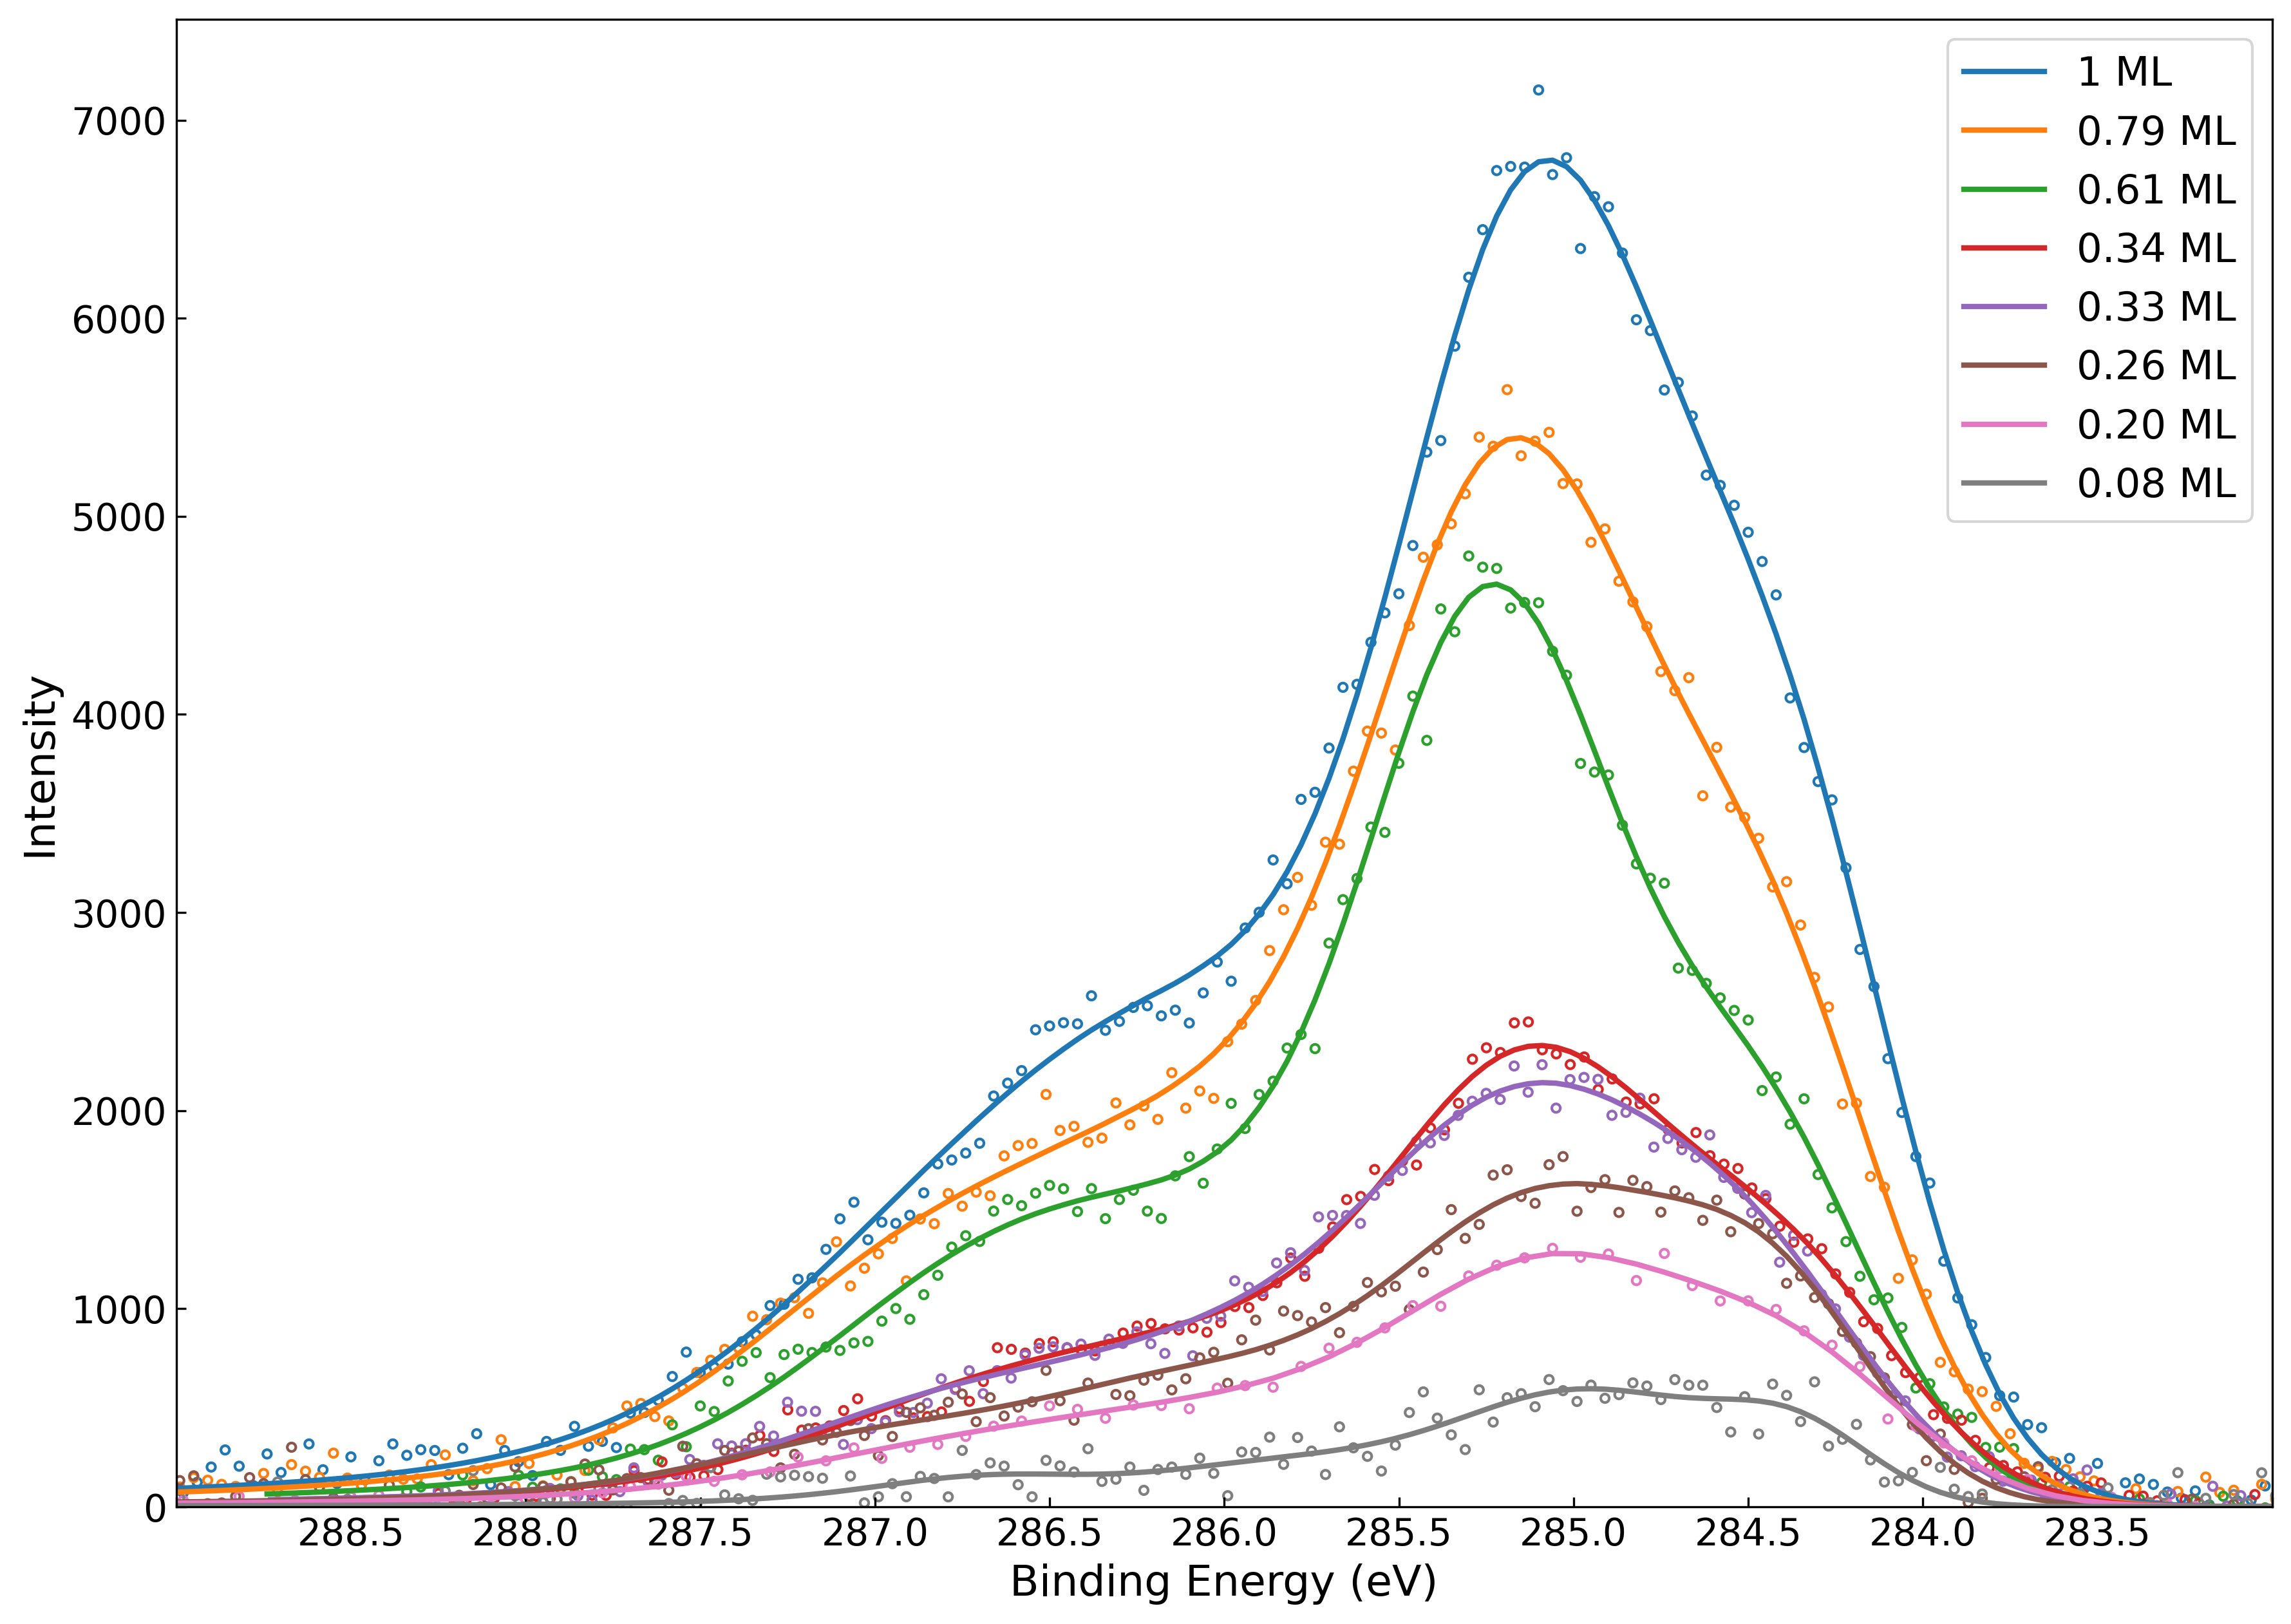
\includegraphics[width=0.85\textwidth]{images/C1s-alpha-comparison.png}
	\caption{Overview of C1s \ac{XPS} spectra for all preparation of the $\alpha$-phase of \ac{QA} on Ag(100).}
	\label{fig:C1s-comparison}
\end{figure}

The \ac{XPS} spectrum for a coverage of 1~\ac{ML} in \autoref{fig:C1s-alpha} demonstrates different peaks that also present carbon atoms with different chemical environments in \ac{QA}.

\begin{figure}[H]
	\centering
	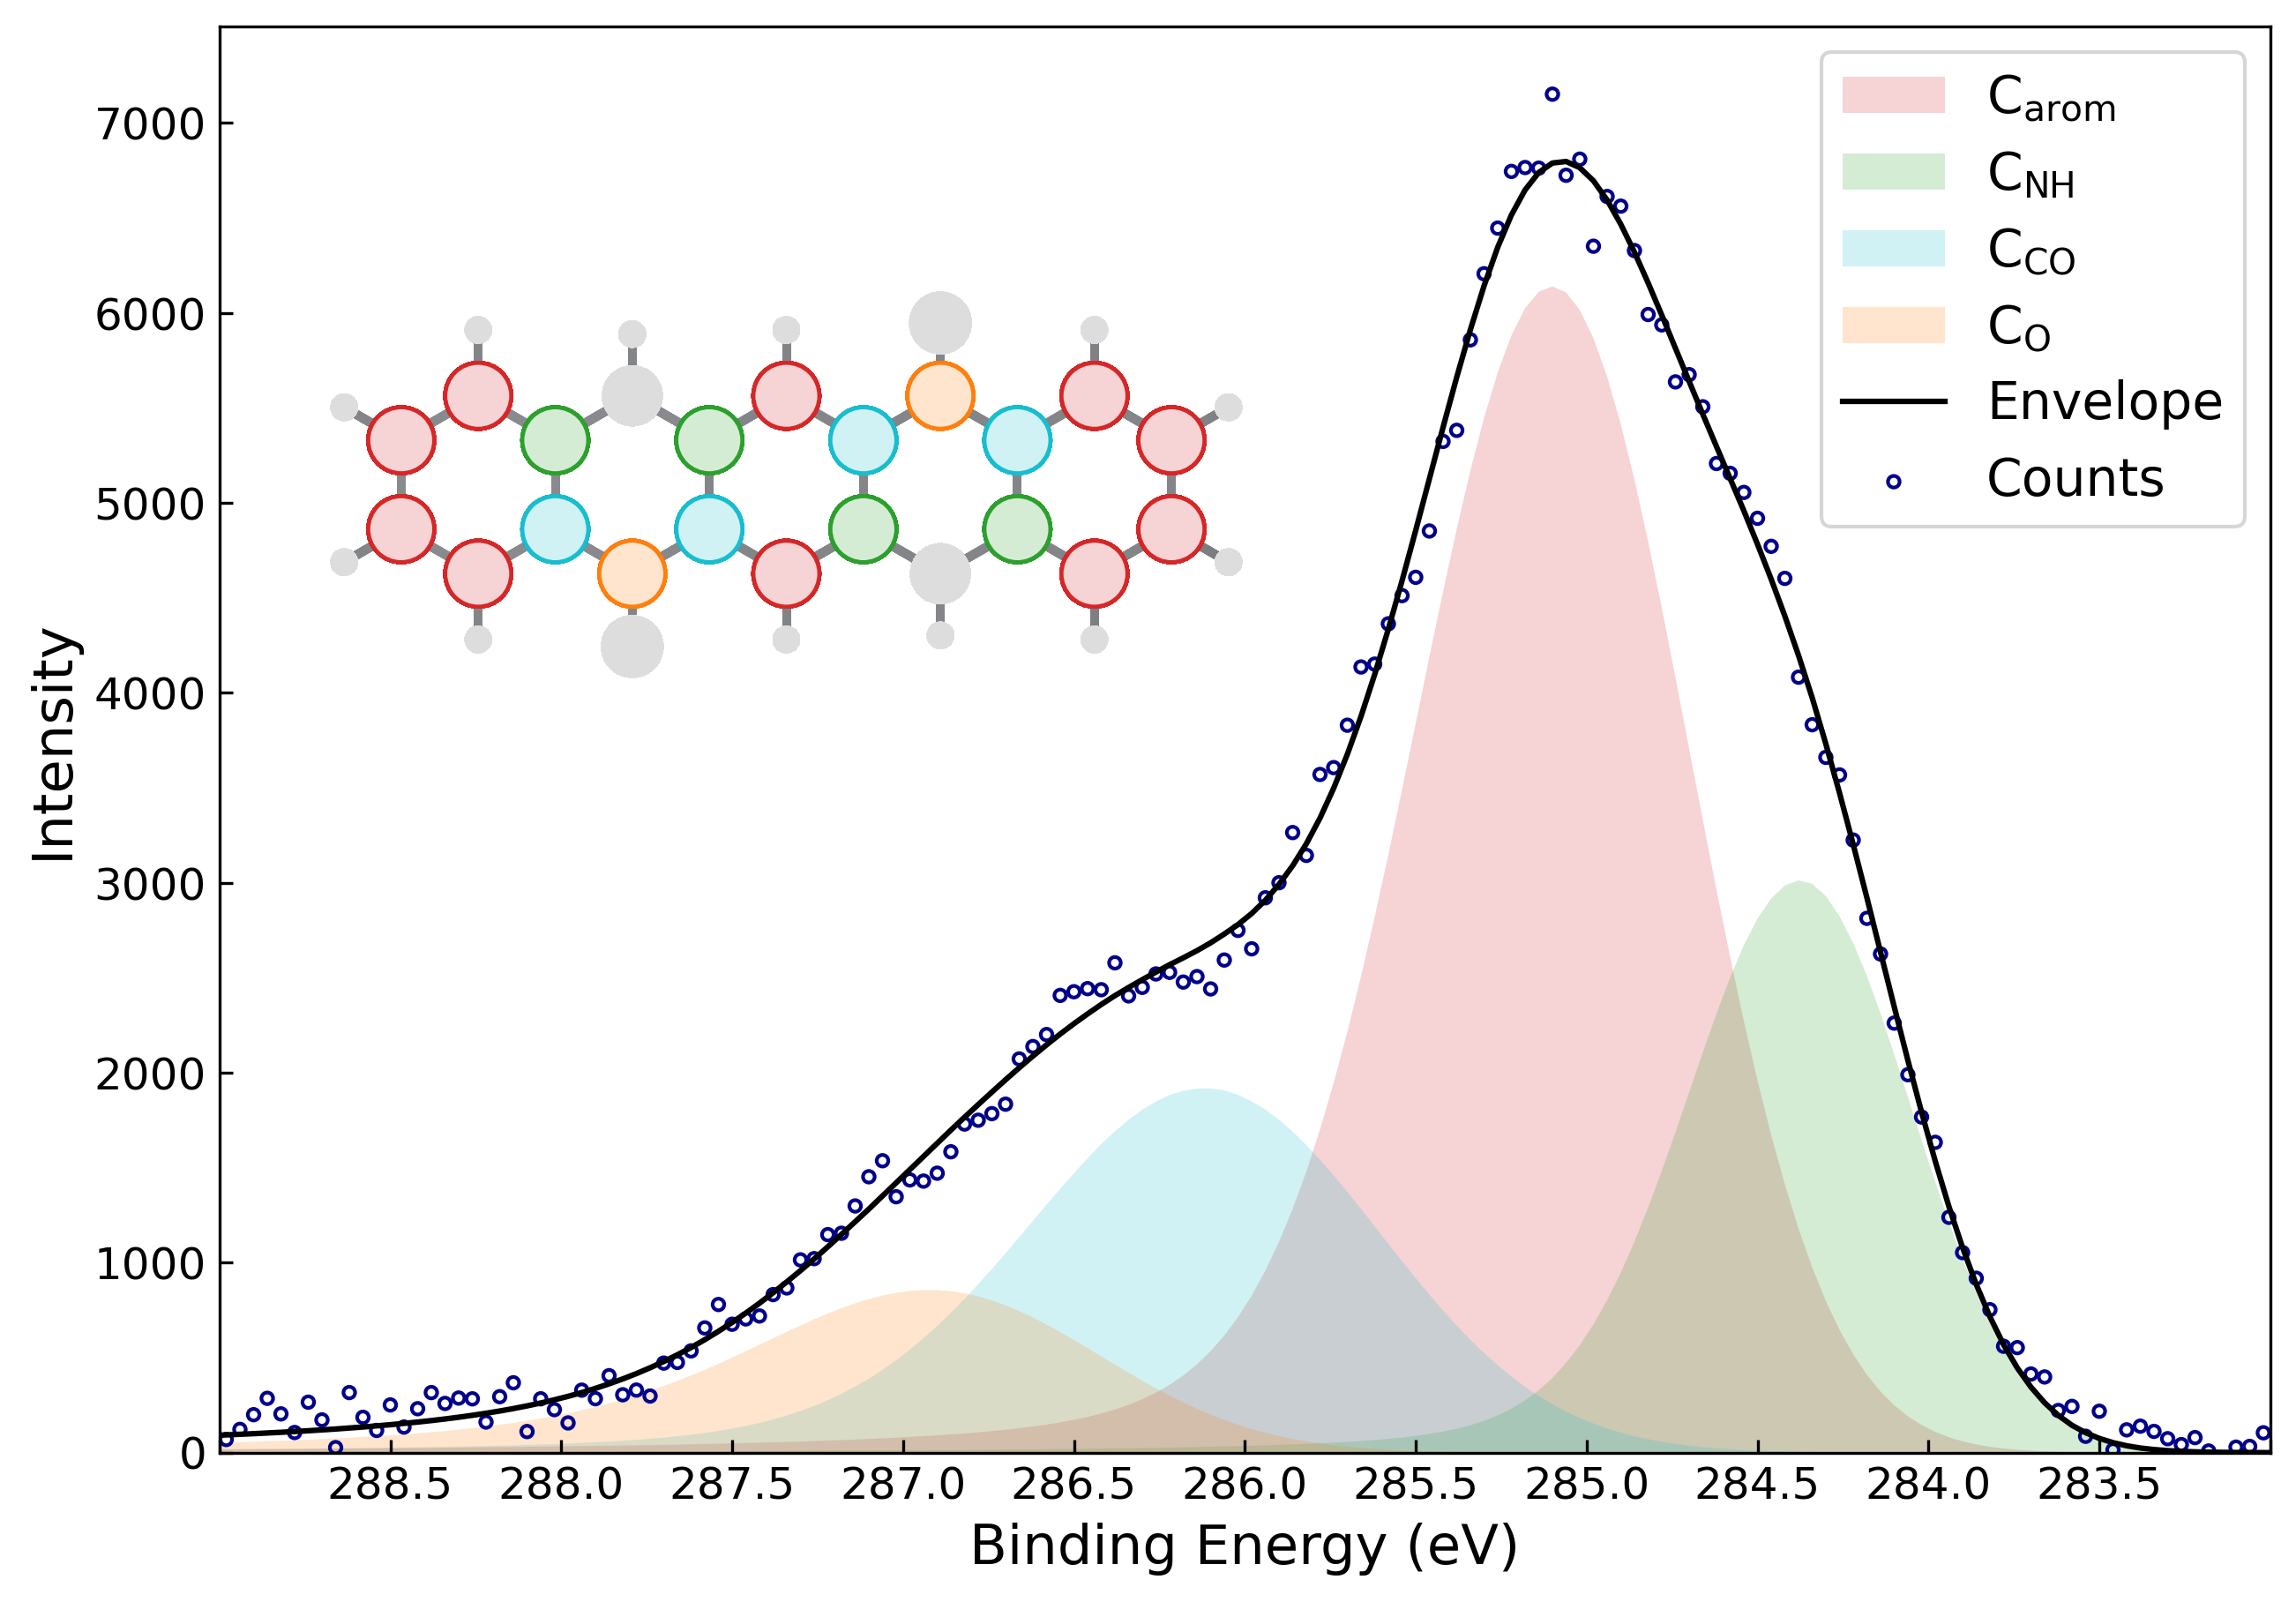
\includegraphics[width=0.85\textwidth]{images/C1s-alpha-P1.png}
	\caption{C1s \ac{XPS} spectrum for the $\alpha$-phase of \ac{QA} on Ag(100) for a coverage of 1~\ac{ML}.}
	\label{fig:C1s-alpha}
\end{figure}

The \ac{XPS} spectra for the C1s photoemission lines of \ac{QA} on Ag(100) reveals consistent spectral features. The main peak ($\mathrm{C_{arom}}$) contains the carbon atoms from the aromatic system that are not part of the ring containing the keto and the amine groups. Next, there is a peak for the two atoms next to the amine ($\mathrm{C_{NH}}$) and another peak for the two atoms next to the ketone ($\mathrm{C_{CO}}$). Finally, there is one peak for the carbon atoms of the ketone ($\mathrm{C_{O}}$). The values corresponding to each peak can be found in \autoref{tab:C1s-alpha-fit}.

\begin{table}[H]
	\centering
	\caption{Fit parameter used in CasaXPS\autocite{CasaSoftwareLtd2022} for the $\alpha$-phase of \ac{QA} on Ag(100) for the C1s photoemission lines.}
	\begin{tabular}{|c|c|c|c|}
		\hline
		peak & \ac{BE} / eV & area ratio & FWHM / eV \\
		\hline
		$\mathrm{C_{arom}}$ & 285.016 & 10 & 0.938 \\ \hline
		$\mathrm{C_{NH}}$ & 284.308 & 4 & 0.764 \\ \hline
		$\mathrm{C_{CO}}$ & 286.010 & 4 & 1.200 \\ \hline
		$\mathrm{C_{O}}$ & 286.723 & 2 & 1.152 \\ \hline
	\end{tabular}
	\label{tab:C1s-alpha-fit}
\end{table}

As illustrated in \autoref{fig:C1s-alpha} and \autoref{tab:C1s-alpha-fit}, the detailed fitting model can be described as follows:
The \ac{BE} of the $\mathrm{C_{arom}}$ peak is measured at 285.016~\si{\eV}, with a \ac{FWHM} of 0.938~\si{\eV}. The $\mathrm{C_{NH}}$ peak is next to the aforementioned peak, with a \ac{BE} of 284.308~\si{\eV} and a \ac{FWHM} of 0.764~\si{\eV}. The analysis of the data reveals that the $\mathrm{C_{CO}}$ peak is located to the left of the $\mathrm{C_{arom}}$ peak. The \ac{BE} of the $\mathrm{C_{CO}}$ peak is 286.010~\si{\eV} and its \ac{FWHM} is 1.200~\si{\eV}. The $\mathrm{C_{O}}$ peak is located to the left of this peak at a \ac{BE} of 286.723~\si{\eV} and a \ac{FWHM} of 1.152~\si{\eV}.

In contrast to the $\alpha$-phase C1s \ac{XPS} spectra of the monolayer, the multilayer spectrum in \autoref{fig:C1s-alpha-multilayer} exhibits a divergent shape.

\begin{figure}[H]
	\centering
	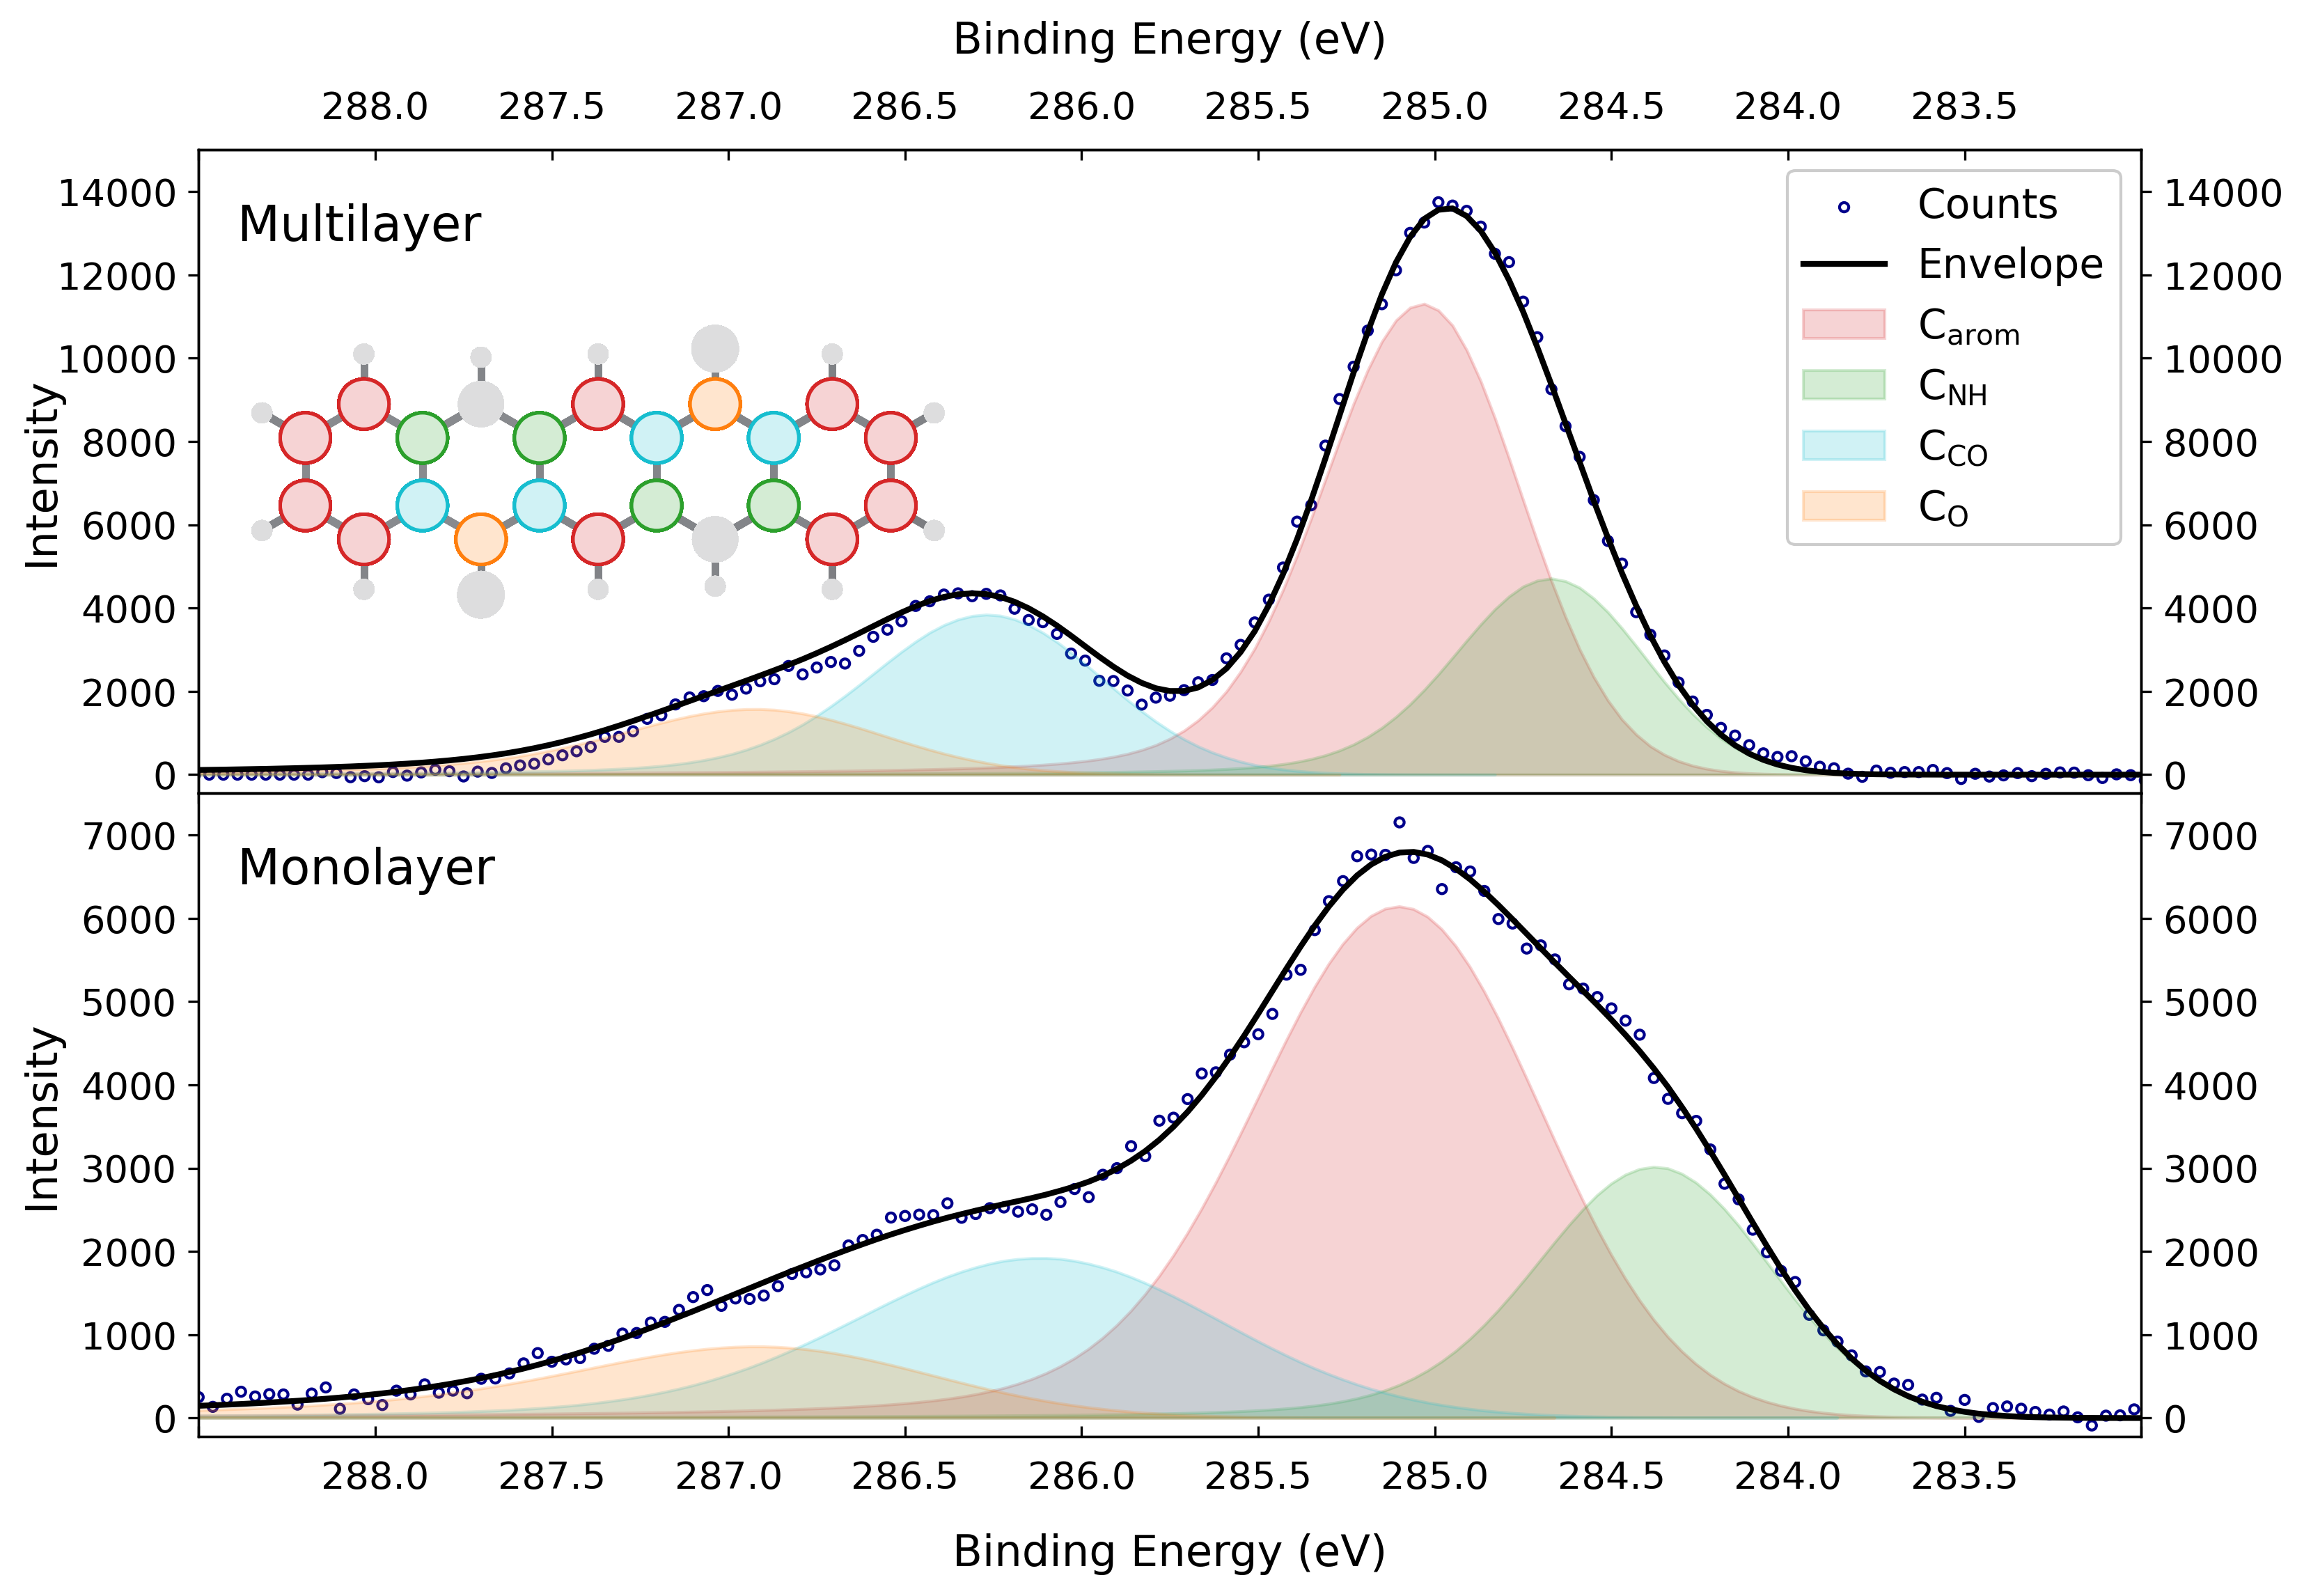
\includegraphics[width=0.9\textwidth]{images/C1s-multilayer.png}
	\caption{C1s \ac{XPS} spectrum for the $\alpha$-phase of \ac{QA} on Ag(100) for a mutlilayer coverage compared to the \ac{XPS} spectrum for a coverage of 1~\ac{ML}.}
	\label{fig:C1s-alpha-multilayer}
\end{figure}

Initially, the multilayer spectrum can still be adequately characterized by using the four distinct peaks, which possess equivalent area ratios to those of the monolayer spectrum. However, it is evident that the multilayer spectrum exhibits a significantly heightened intensity relative to the monolayer spectrum. The primary distinctions are evident in the \ac{BE} and the \ac{FWHM} of the peaks. The spectrum displays a discernible minimum between the aromatic carbon peak $\mathrm{C_{arom}}$ and the carbonyl carbon peak $\mathrm{C_{O}}$. The peak associated with the amine group ($\mathrm{C_{NH}}$) exhibits a shift towards the $\mathrm{C_{arom}}$ peak.


\cleardoublepage
\subsection{O1s spectra}

\autoref{fig:O1s-comparison} presents a series of \ac{XPS} spectra for the O1s photoemission lines of \ac{QA} at three different coverages: 0.33~\ac{ML}, 0.79~\ac{ML} and 1~\ac{ML}. A prominent peak centered near 531~\si{\eV} is exhibited by all spectra, a characteristic of the oxygen atoms in carbonyl functional groups present in the \ac{QA} molecule. Additionally, the shape of the peak suggests the presence of a more intricate structure than a single peak. The spectra exhibit a comparable overall shape and peak position across the various surface coverages.

As anticipated, the spectral intensity increases with coverage, indicative of an increased number of \ac{QA} molecules adsorbed on the surface. Beyond the intensity changes, differences in peak width and asymmetry are also observed. The spectrum at the lowest coverage (0.33~\si{ML}) is narrower and more symmetric, whereas the spectra at higher coverages become progressively broader and more asymmetric.

In summary, the O1s \ac{XPS} spectra of \ac{QA} on Ag(100) are qualitatively similar across coverages. A peak assignment and more detailed evaluation will be provided in a subsequent part to elucidate the specific spectral components contributing to the observed features.

\begin{figure}[H]
	\centering
	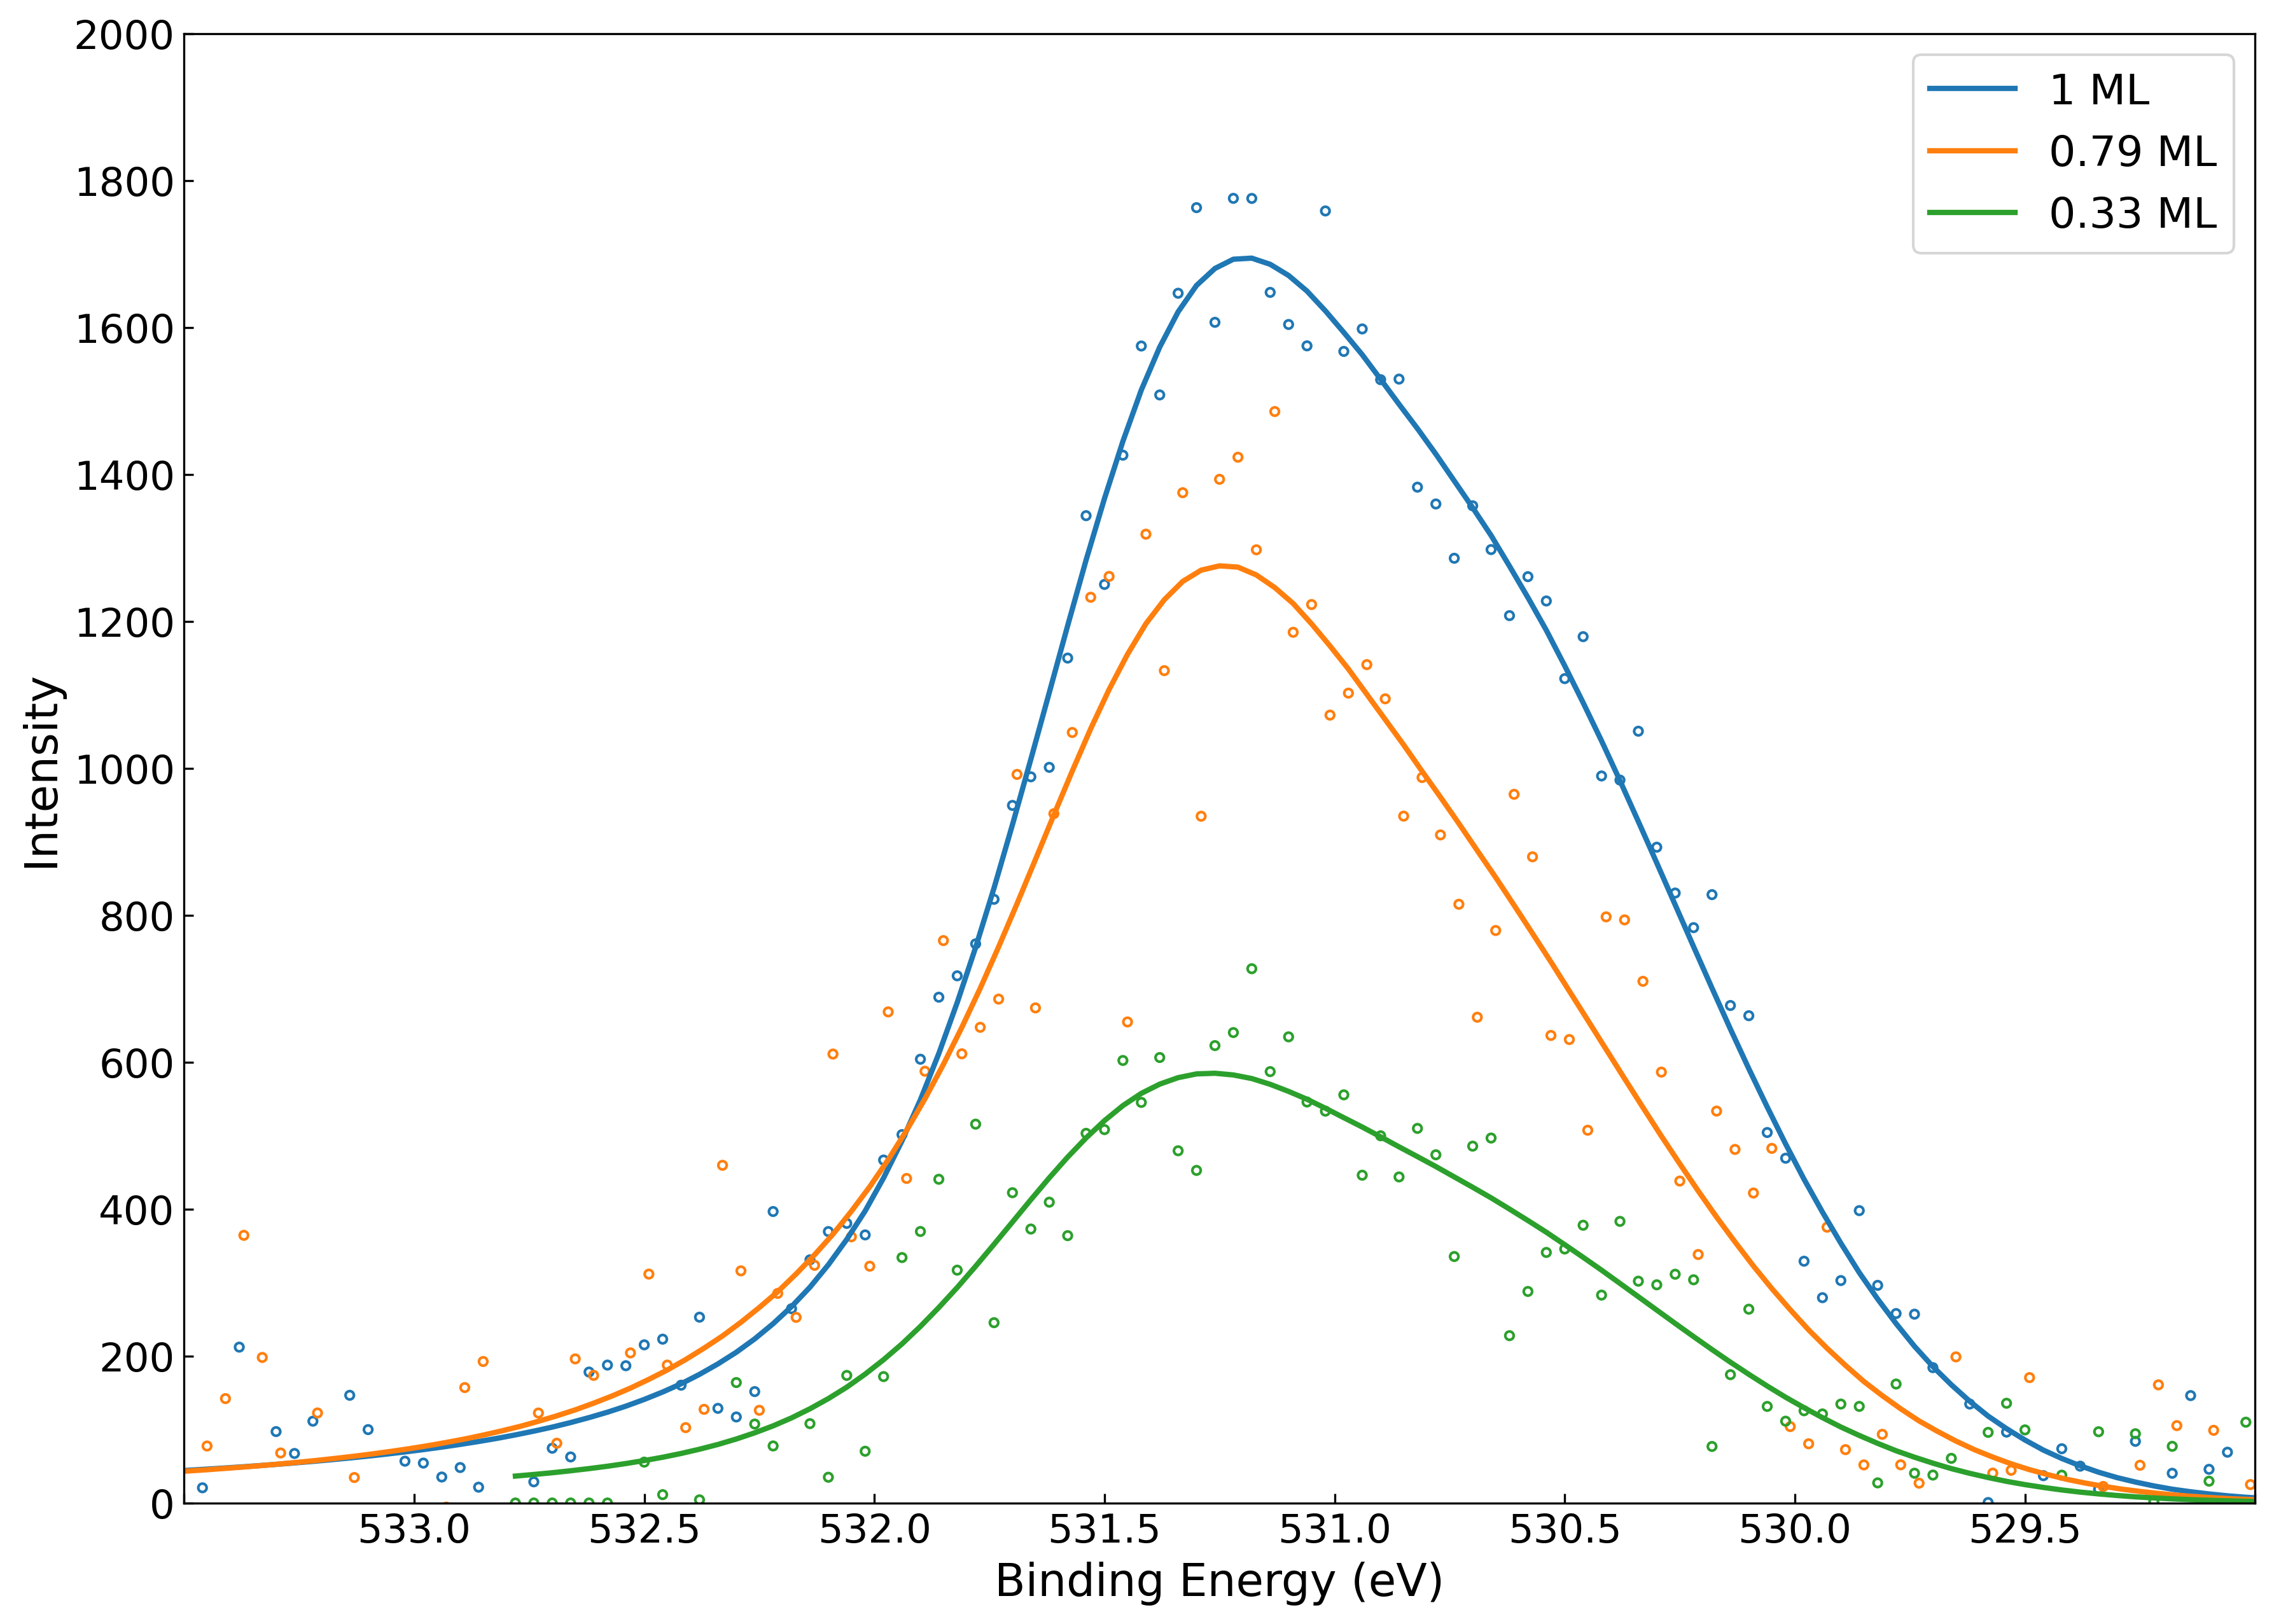
\includegraphics[width=0.9\textwidth]{images/O1s-alpha-comparison.png}
	\caption{Overview of O1s \ac{XPS} spectra for all preparation of the $\alpha$-phase of \ac{QA} on Ag(100)}
	\label{fig:O1s-comparison}
\end{figure}

A detailed O1s spectrum of \ac{QA} on Ag(100) at a 1~\ac{ML} coverage reveals two distinguishable spectral components, which is shown in \autoref{fig:O1s-alpha}.

\begin{figure}[H]
	\centering
	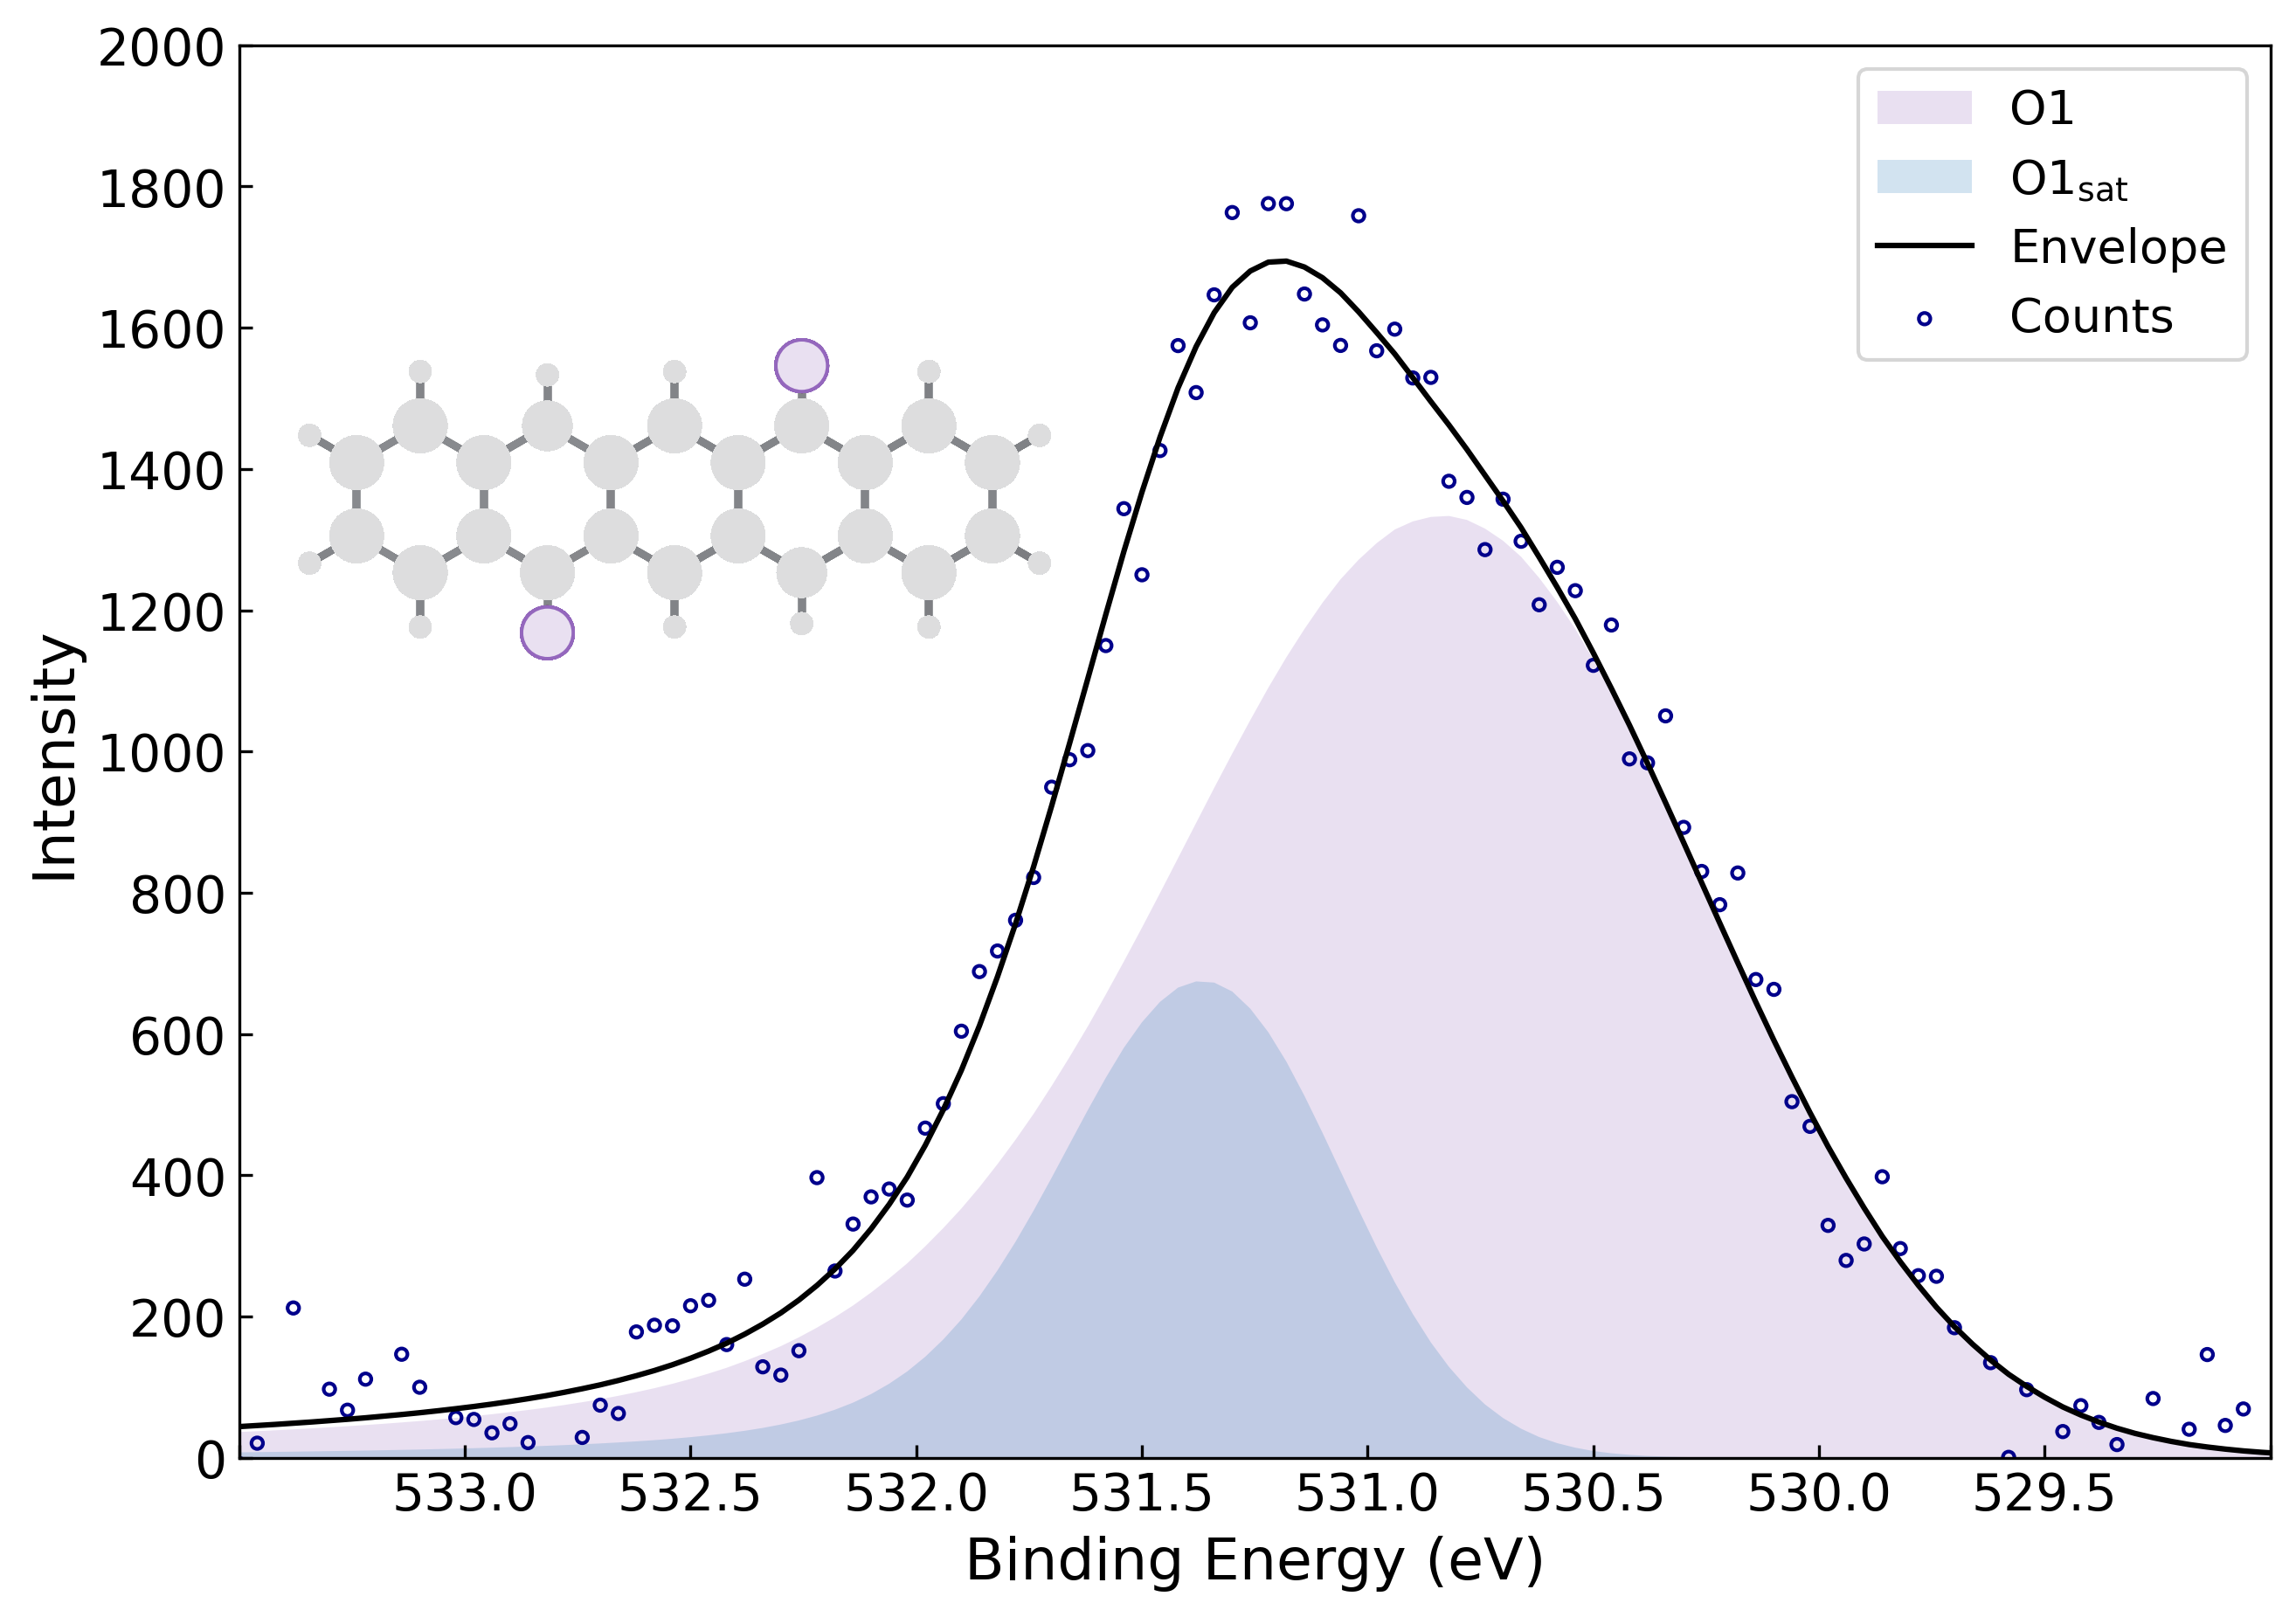
\includegraphics[width=0.9\textwidth]{images/O1s-alpha-P1.png}
	\caption{O1s \ac{XPS} spectrum for the $\alpha$-phase of \ac{QA} on Ag(100) for a coverage of 1~\ac{ML}.}
	\label{fig:O1s-alpha}
\end{figure}

As illustrated in \autoref{fig:O1s-alpha} and \autoref{tab:O1s-alpha-fit}, the primary component ($\mathrm{O1}$) is at a \ac{BE} of 530.657~\si{\eV}, exhibiting a \ac{FWHM} of 1.360~\si{\eV}. This peal is attributed to the core-level photoemission from oxygen atoms situated within carbonly functionalities. The relatively broad linewidth is indicative of slight variations in the local chemical environment of these oxygen atoms.

A secondary, less intense component ($\mathrm{O1_{sat}}$) is observed at a higher \ac{BE} of 531.273~\si{\eV} with a narrower \ac{FWHM} of 0.712~\si{\eV}. This feature is interpreted as a shake-up satellite, arising from e.g. a $\pi-\pi^*$ transition within the conjugated $\pi$ system of the \ac{QA} molecule.

Quantitative analysis of the peak areas reveals that the satellite-to-main peak area ratio is approximately 0.27, which is equivalent to 21~\% of the total O1s intensity. This ratio is consistent with the expected intensity of shake-up features in aromatic systems with significant conjugation.\autocite{Bauer2014}

The combination of these two components provides a comprehensive representation of the O1s photoemission lines of \ac{QA}. This representation reflects both the intrinsic chemical identity of the oxygen atoms and the dynamic electron processes that accompany core-level photoemission.

\begin{table}[H]
	\centering
	\caption{Fit parameter used in CasaXPS\autocite{CasaSoftwareLtd2022} for the $\alpha$-phase of \ac{QA} on Ag(100) for the O1s photoemission lines..}
	\begin{tabular}{|c|c|c|c|}
		\hline
		peak & \ac{BE} / eV & area ratio & FWHM / eV \\
		\hline
		$\mathrm{O1}$ & 530.657 & 2.00 & 1.360 \\ \hline
		$\mathrm{O1_{sat}}$ & 531.273 & 0.53 & 0.712 \\ \hline
	\end{tabular}
	\label{tab:O1s-alpha-fit}
\end{table}

In \autoref{fig:O1s-alpha-multilayer}, a \ac{XPS} spectrum with a multilayer coverage is compared to the previously discussed \ac{XPS} spectrum.

\begin{figure}[H]
	\centering
	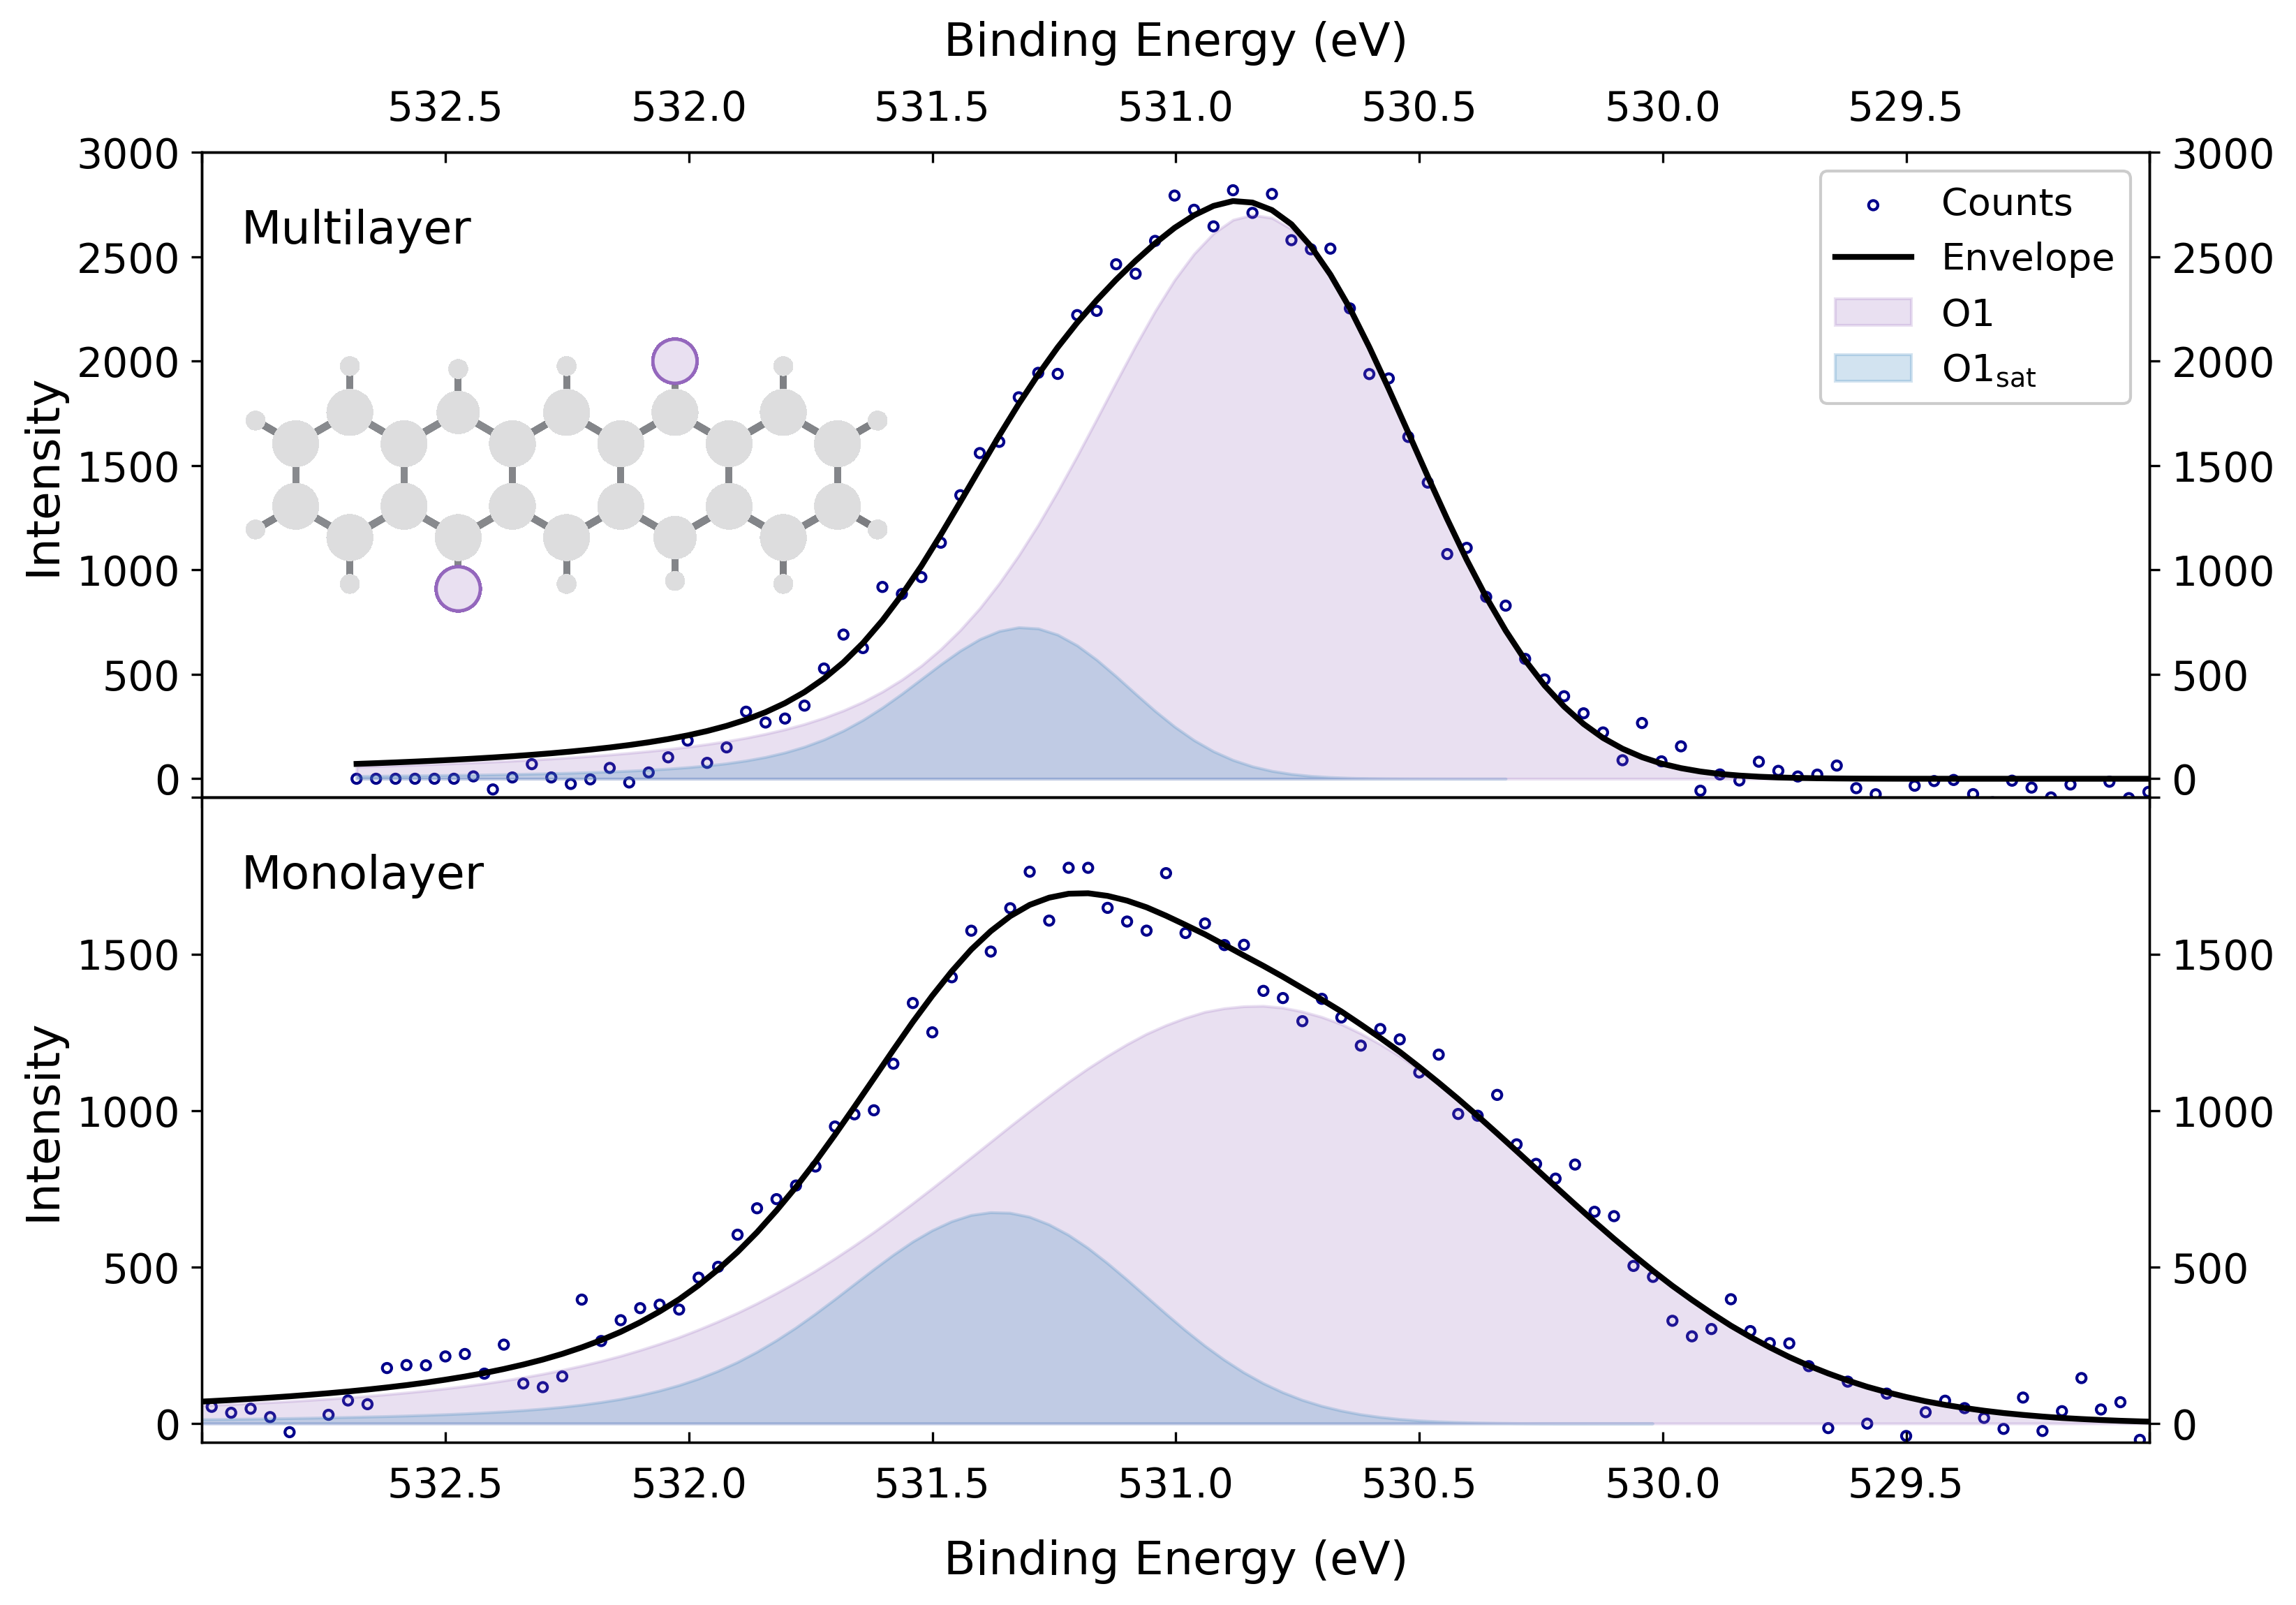
\includegraphics[width=0.84\textwidth]{images/O1s-multilayer.png}
	\caption{O1s \ac{XPS} spectrum for the $\alpha$-phase of \ac{QA} on Ag(100) for a mutlilayer coverage compared to the \ac{XPS} spectrum for a coverage of 1~\ac{ML}.}
	\label{fig:O1s-alpha-multilayer}
\end{figure}

The O1s \ac{XPS} spectrum recorded for \ac{QA} on Ag(100) at multilayer coverage reveals a well-defined structure characterized by two distinct photoemission peaks. The primary component ($\mathrm{O1}$) is at a \ac{BE} of 530.733~\si{\eV} and a \ac{FWHM} of 0.75~\si{\eV}. In comparison with the \ac{ML} $\mathrm{O1}$ peak, the peak position undergoes a change of approximately 0.076~\si{\eV}. A more salient finding is the change in the \ac{FWHM} of approximately 0.61~\si{\eV}, which nearly corresponds to a 50~\% alteration.

 The satellite peak ($\mathrm{O1_{sat}}$) is observed at 531.24~\si{\eV} with a \ac{FWHM} of 0.5~\si{\eV}. Once more, the position of the $\mathrm{O1_{sat}}$ peak in relation to the \ac{ML} remains constant. However, the \ac{FWHM} of the peak decreases by 0.21~\si{\eV}, which corresponds to approximately 30~\%. This alteration may be attributable to the enhanced intensity exhibited by the multilayer \ac{XPS} spectrum. The satellite-to-main ratio experiences a decrease from 0.27 in the \ac{ML} to 0.18 in the multilayer, indicating a reduced skake-up process.

\cleardoublepage
\subsection{N1s spectra}

The \ac{XPS} spectra displayed in \autoref{fig:N1s-comparison} show the N1s photoemission lines of \ac{QA} on Ag(100) with varying coverages between 0.26~\ac{ML} and 1~\ac{ML}. A prominent main peak centered around 400~\si{\eV} is exhibited by all spectra. Despite the general spectral similarities across different coverages, clear distinctions emerge in the shape and intensity of the main peak. As the coverage increases from submonolayer to monolayer, the main peak systematically increases in intensity, reflecting the proportional increase in nitrogen-containing molecules. In scenarios where coverages are less substantial, the spectra tend to manifest as marginally broader. Conversely, as the coverage increases, the spectra become more narrow.

Additionally, a secondary peak is evident on the low-\ac{BE} side of the main peak in some spectra at approximately 398~\si{\eV}. In summary, while the core features of the \ac{XPS} of \ac{QA} remain largely preserved across different coverages, changes are observed in peak intensity and width, in addition to the second peak at a lower \ac{BE}.

\begin{figure}[H]
	\centering
	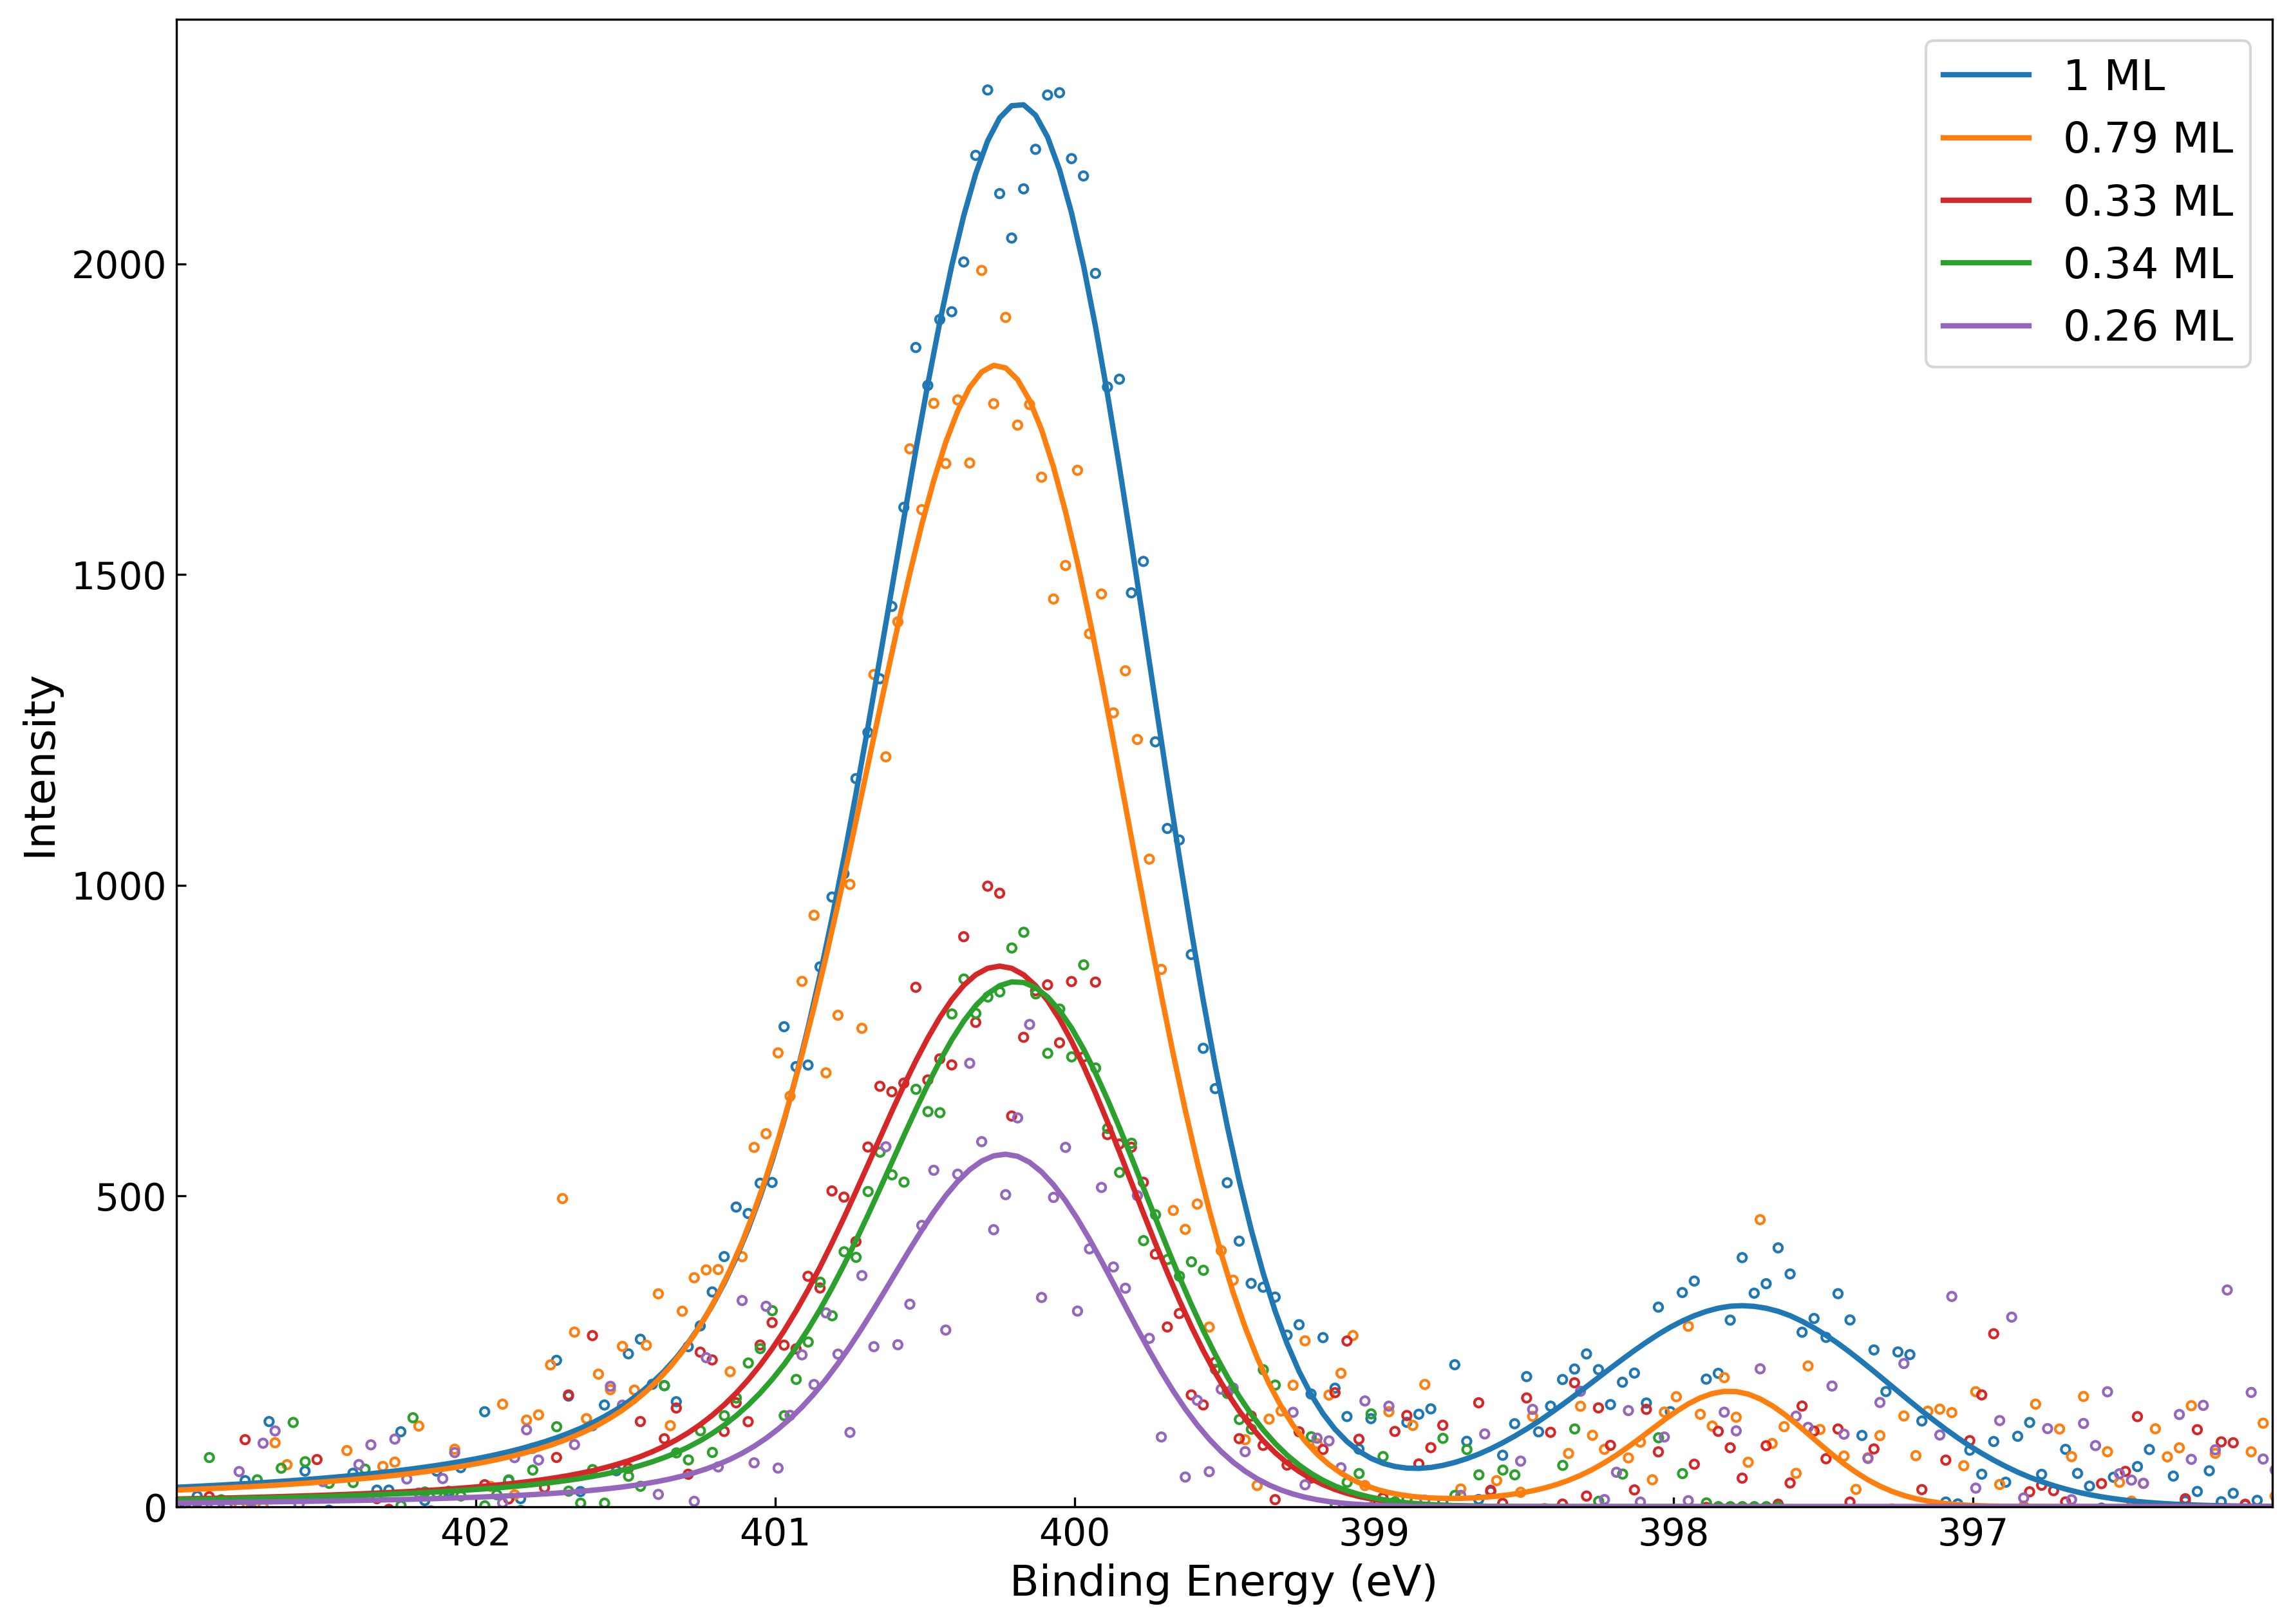
\includegraphics[width=0.9\textwidth]{images/N1s-alpha-comparison.png}
	\caption{Overview of N1s \ac{XPS} spectra for all preparation of the $\alpha$-phase of \ac{QA} on Ag(100)}
	\label{fig:N1s-comparison}
\end{figure}

The N1s \ac{XPS} spectrum of \ac{QA} on Ag(100) with a coverage of 1~\ac{ML}, as depicted in \autoref{fig:N1s-comparison}, is discussed in more detail in \autoref{fig:N1s-alpha}, which presents the different peaks.

\begin{figure}[H]
	\centering
	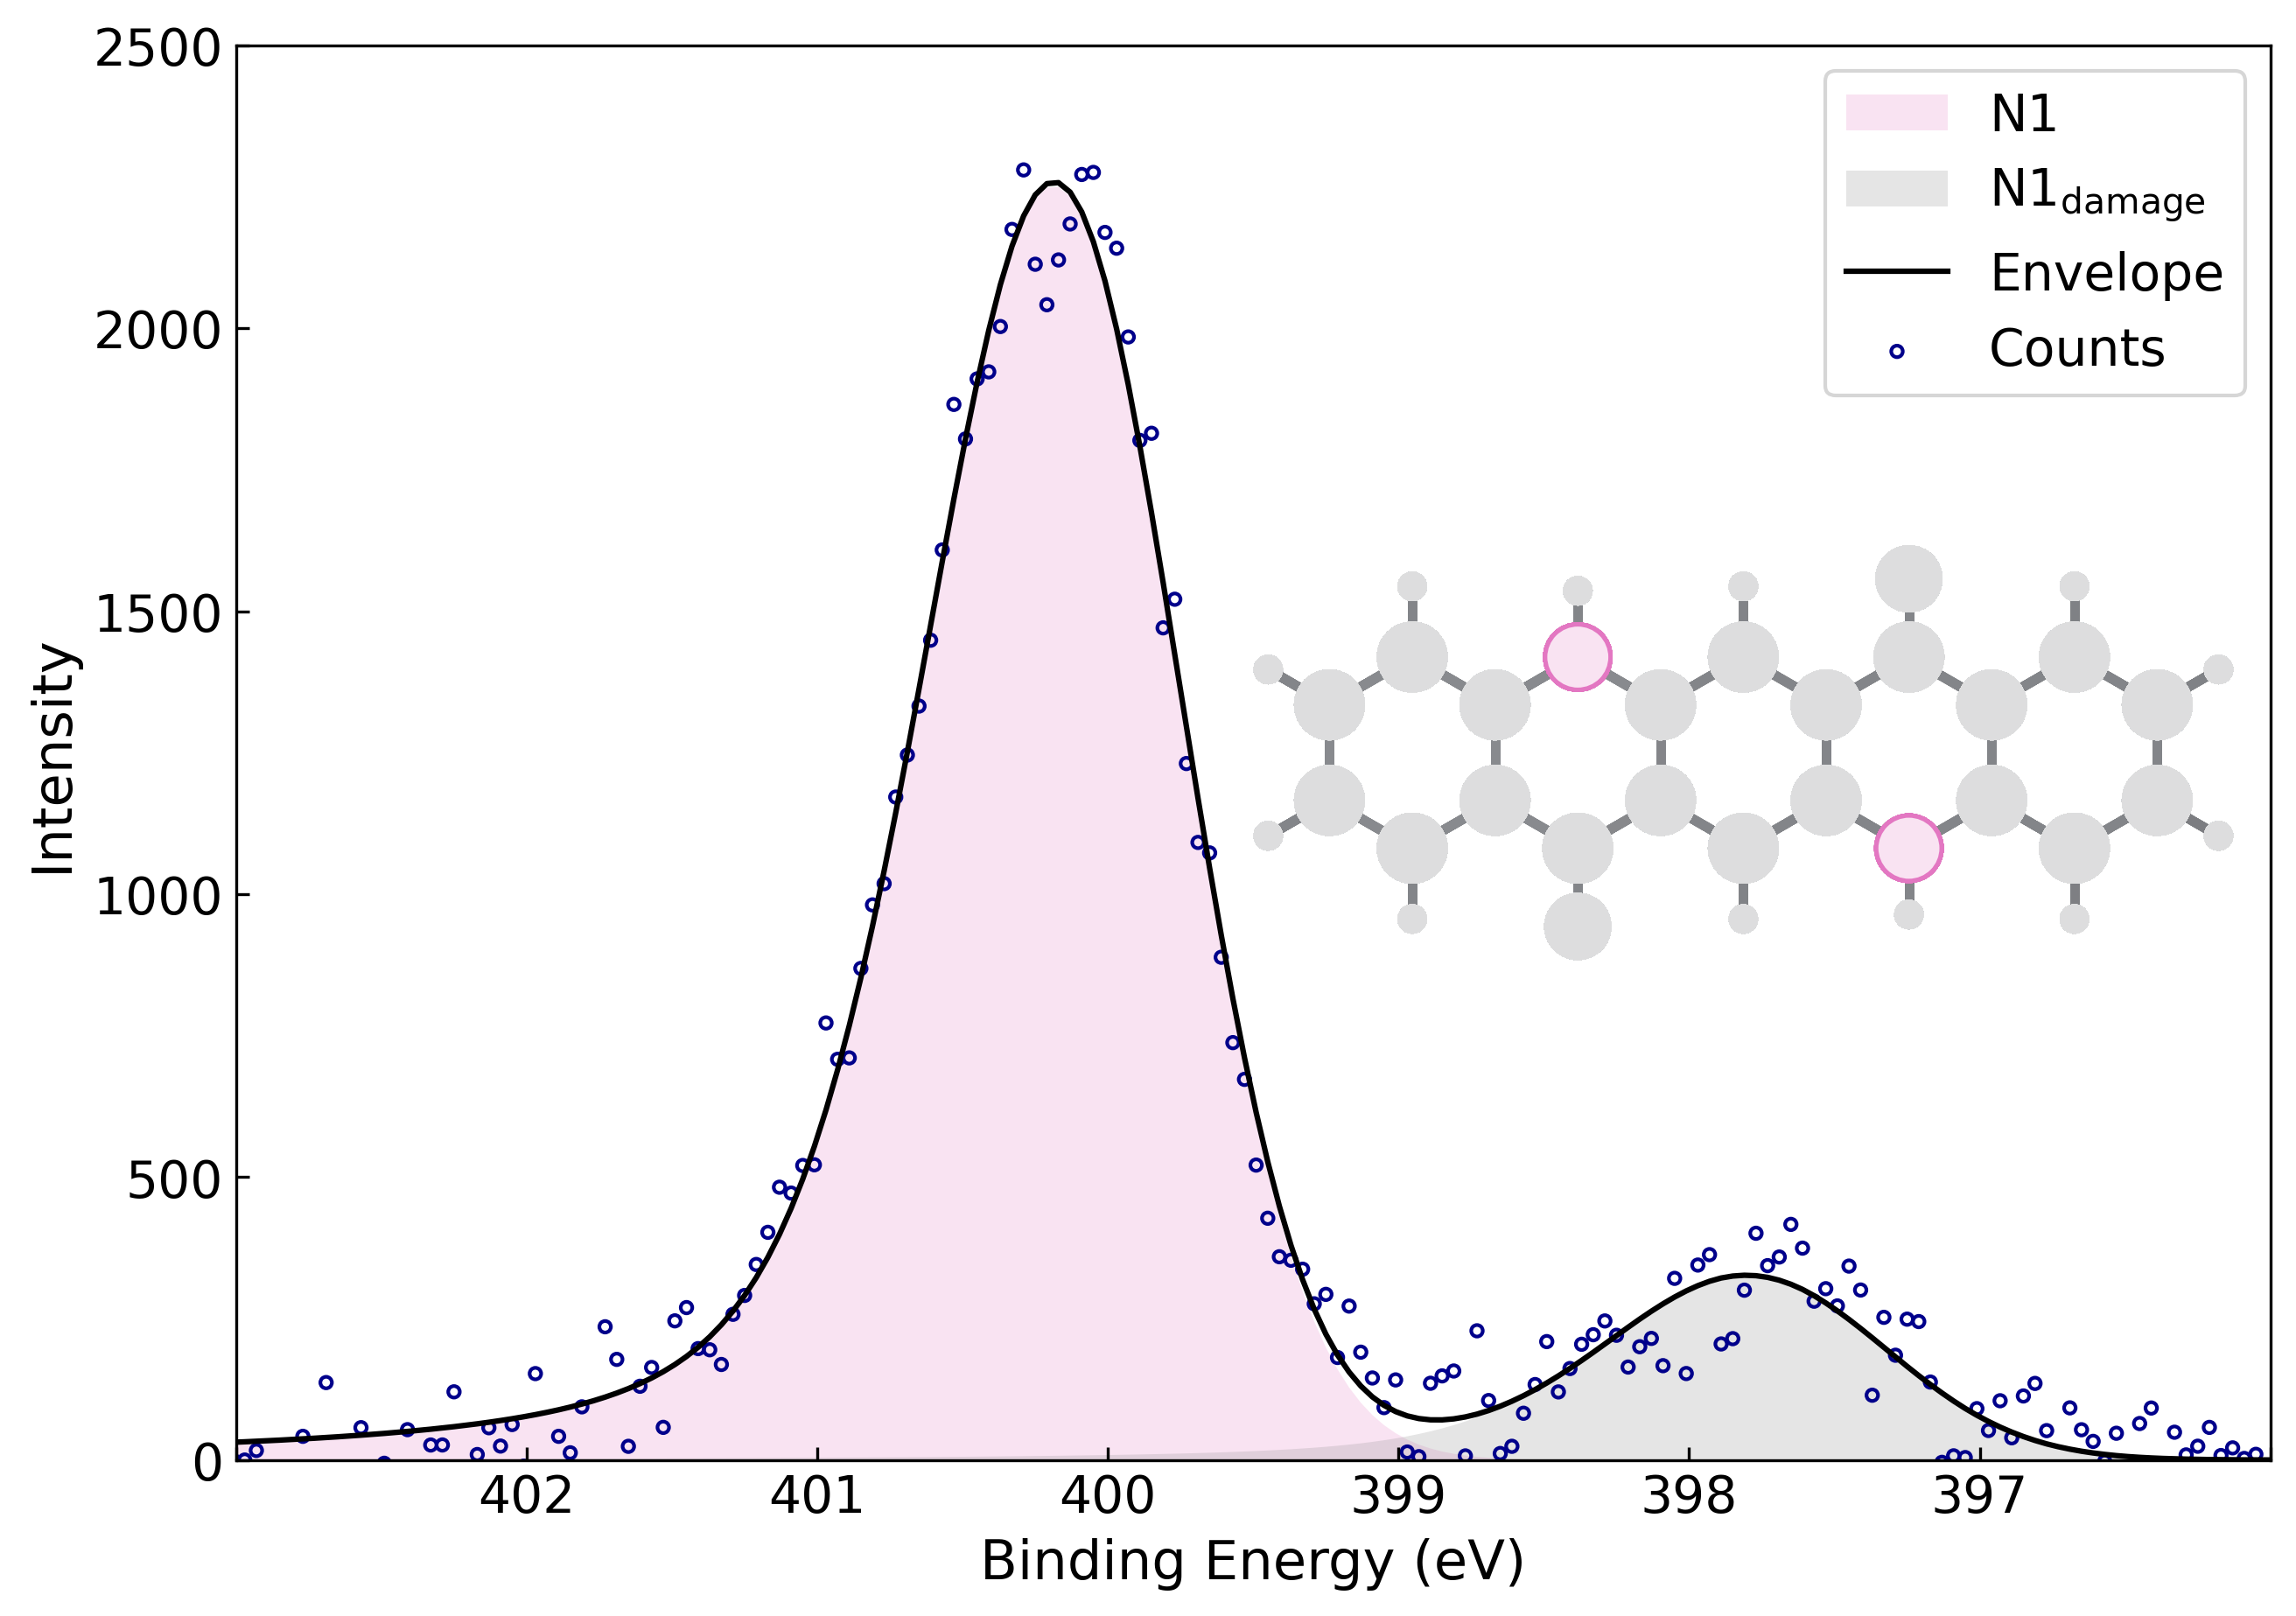
\includegraphics[width=0.9\textwidth]{images/N1s-alpha-P1.png}
	\caption{N1s \ac{XPS} spectrum for the $\alpha$-phase of \ac{QA} on Ag(100) for a coverage of 1~\ac{ML}.}
	\label{fig:N1s-alpha}
\end{figure}

The \ac{XPS} spectrum in \autoref{fig:N1s-alpha} can be divided into two discrete components: a primary peak ($\mathrm{N1}$) and a secondary feature at lower \ac{BE} ($\mathrm{N1_{damage}}$). The precise values for the two peaks are enumerated in \autoref{tab:N1s-alpha-fit}. The $\mathrm{N1}$ peak, with a center at 400.054~\si{\eV} and a \ac{FWHM} of 1.01406~\si{\eV}, is attributed to nitrogen atoms embedded within the chemically intact \ac{QA} molecule. The narrow \ac{FWHM} and symmetrical peak profile are indicative of a well-defined and electronically homogenous nitrogen environment.

The secondary component, $\mathrm{N1_{damage}}$, emerges at a \ac{BE} of 397.656~\si{\eV} and exhibits a \ac{FWHM} of 1.12~\si{\eV},. This phenomenon is attributed to the presence of chemically modified nitrogen species, which are most likely the result of radiation-induced damage due to prolonged X-ray exposure.

A thorough qualitative analysis was conducted, which yielded a damage-intensity-ratio of 0.16. This ratio indicated that the majority of nitrogen atoms maintain their molecular integrity under the measurement conditions, while a minor but significant portion experiences beam damage.

\begin{table}[H]
	\centering
	\caption{Fit parameter used in CasaXPS\autocite{CasaSoftwareLtd2022} for the $\alpha$-phase of \ac{QA} on Ag(100) for the N1s photoemission lines.}
	\begin{tabular}{|c|c|c|c|}
		\hline
		peak & \ac{BE} / eV & area ratio & FWHM / eV \\
		\hline
		$\mathrm{N1}$ & 400.054 & 2.00 & 1.017 \\ \hline
		$\mathrm{N1_{damage}}$ & 397.656 & 0.31 & 1.160 \\ \hline
	\end{tabular}
	\label{tab:N1s-alpha-fit}
\end{table}

A comparison of the N1s \ac{XPS} spectrum of the monolayer and the spectrum corresponding to the multilayer is illustrated in \autoref{fig:N1s-alpha-multilayer}.

\begin{figure}[H]
	\centering
	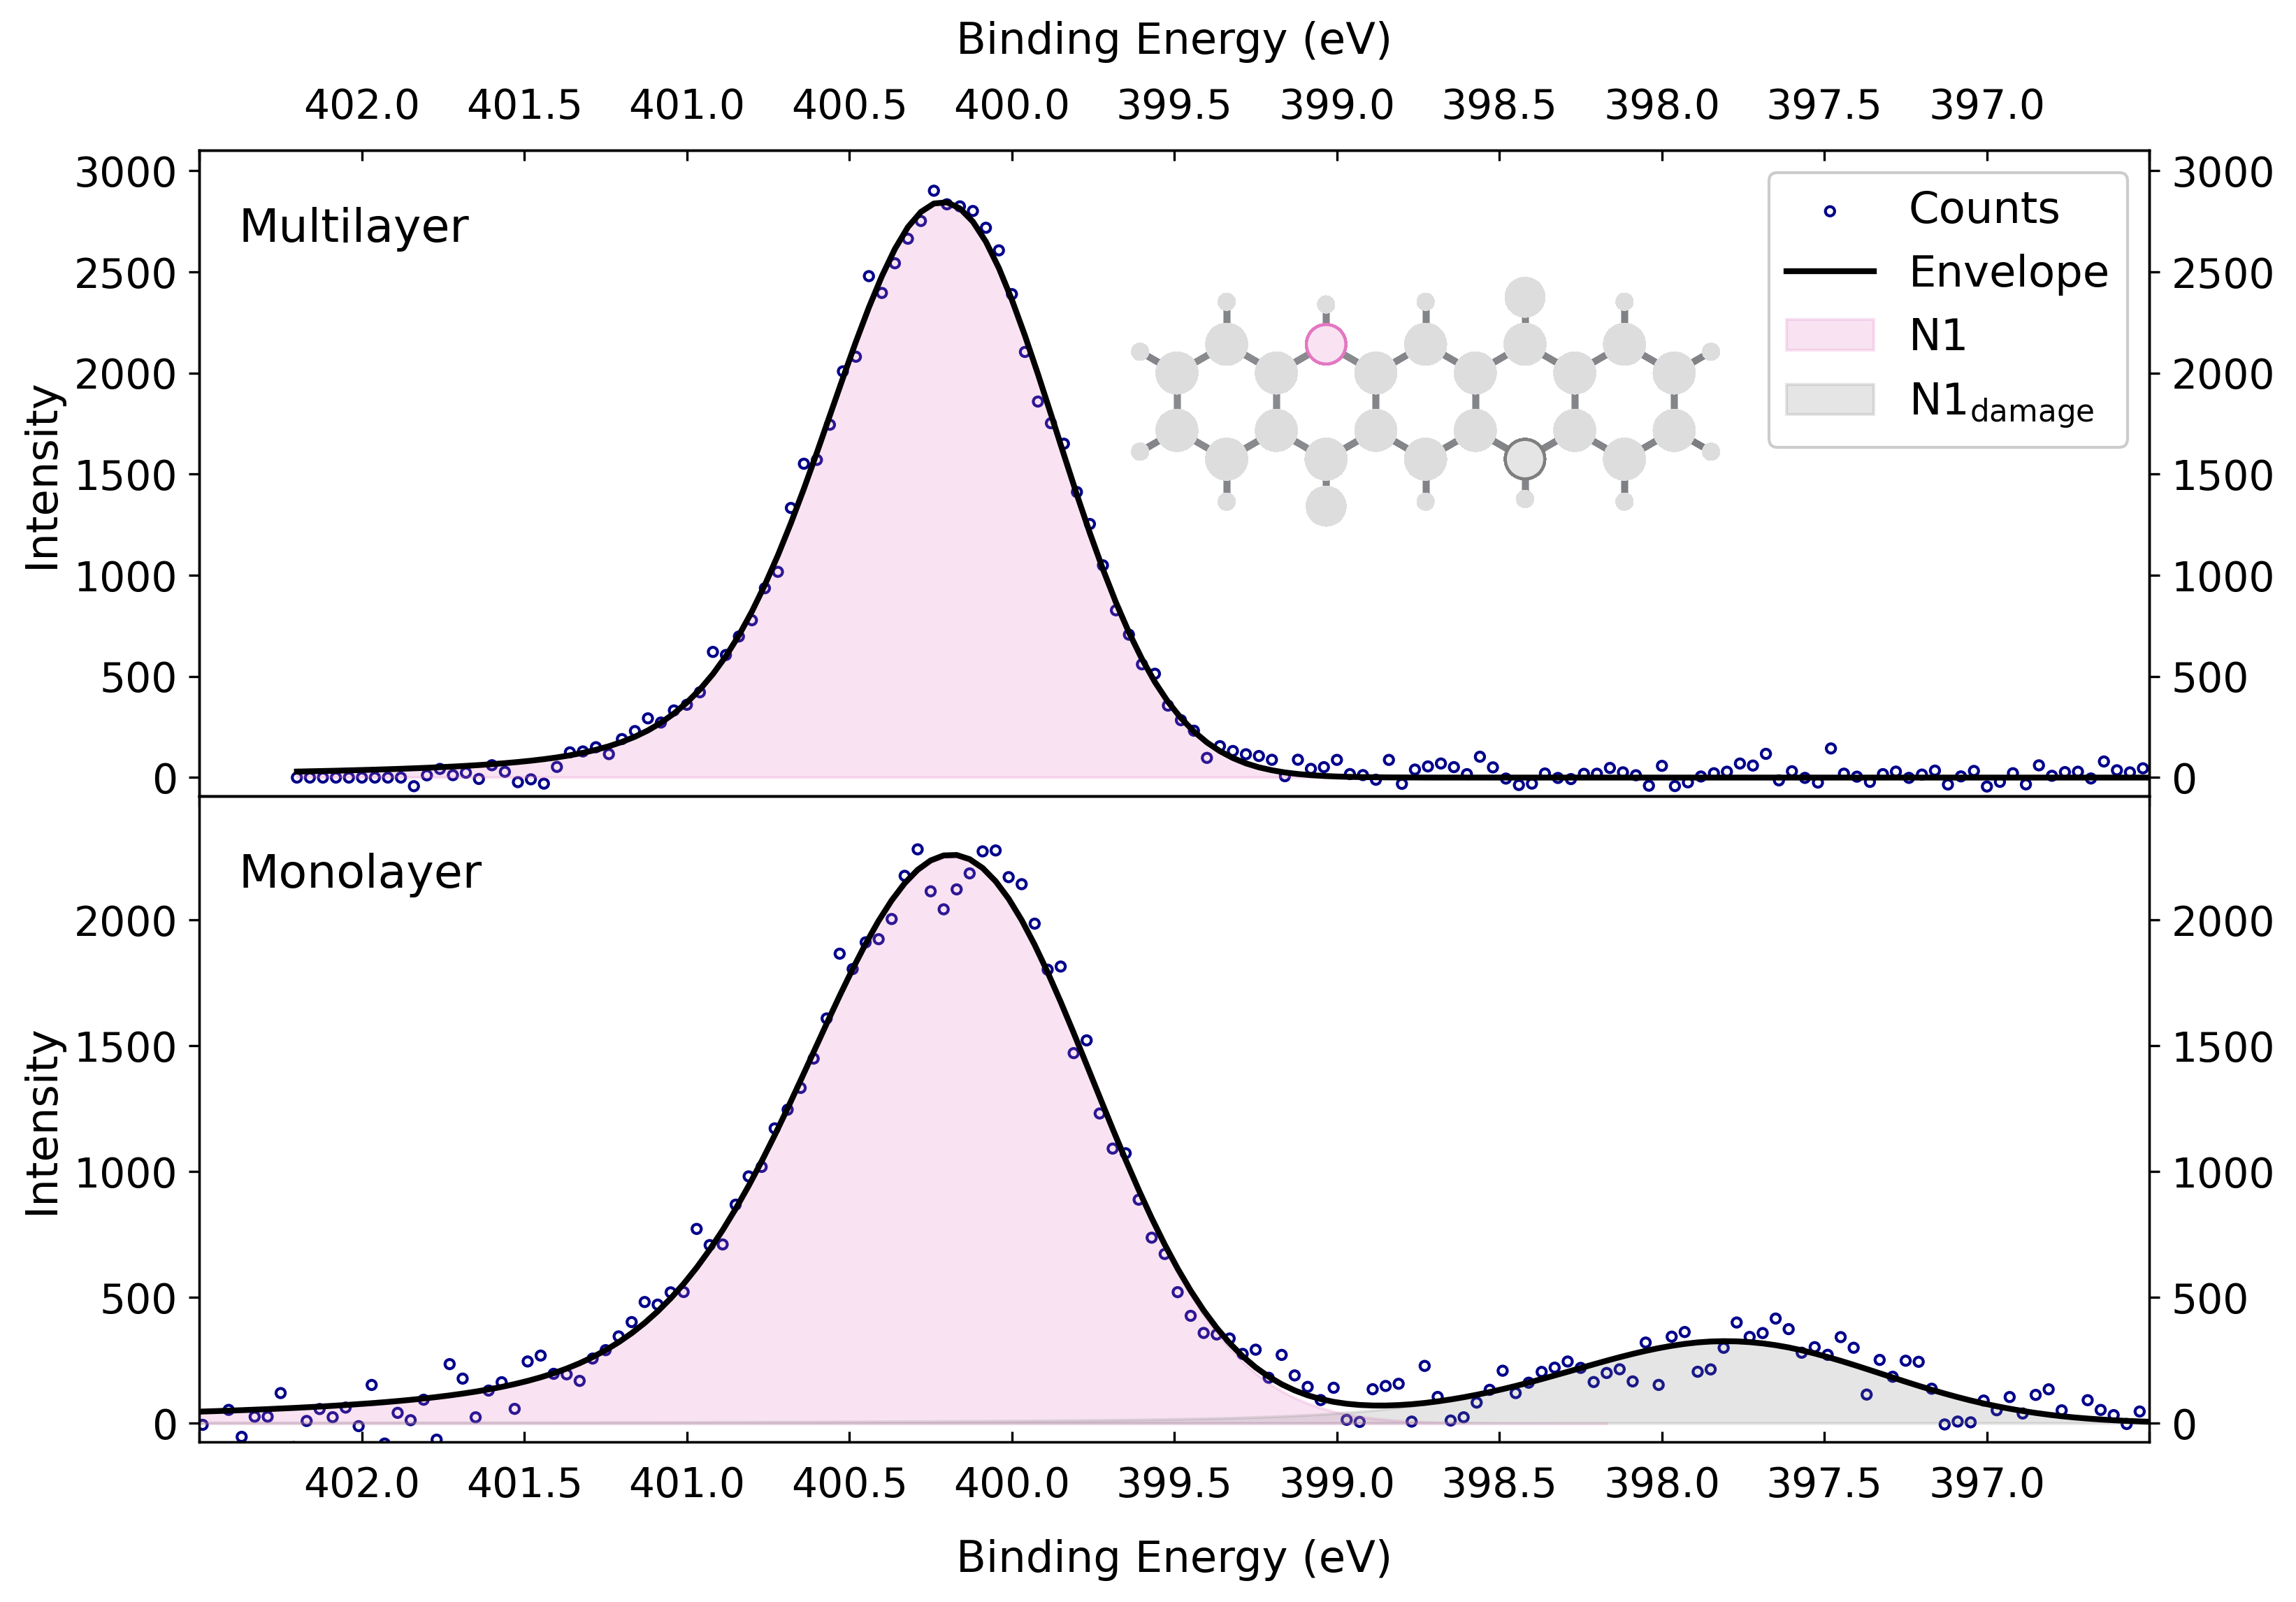
\includegraphics[width=0.9\textwidth]{images/N1s-multilayer.png}
	\caption{N1s \ac{XPS} spectrum for the $\alpha$-phase of \ac{QA} on Ag(100) for a mutlilayer coverage compared to the \ac{XPS} spectrum for a coverage of 1~\ac{ML}.}
	\label{fig:N1s-alpha-multilayer}
\end{figure}

The \ac{XPS} spectrum with a multilayer coverage reveals a single component ($\mathrm{N1}$ centered at a \ac{BE} of 400.147~\si{\eV}, accompanied by a \ac{FWHM} of 0.82~\si{\eV}. This observation signifies a subtle modification in the chemical environment surrounding the nitrogen atom. The peak associated with beam damage ($\mathrm{N1_{damage}}$) remains undetected. This absence indicated that the spectrum of the multilayer originated predominantly from chemically intact nitrogen species. The \ac{BE} exhibits a slight increase (0.93~\si{\eV}) in the multilayer, accompanied by a narrower \ac{FWHM}.


\cleardoublepage
\section{C1s XPS spectra for the phase transition}
\label{sec:res-phase-transition}

The \autoref{fig:C1s-phase-transition} illustrates C1s photoemission lines for \ac{QA} molecules absorbed on an Ag(100) substrate, showing the transition from the $\alpha$- to the $\beta$-phase. The \ac{XPS} spectra are arranged vertically, with the $\alpha$-phase shown at the top, the $\beta$-phase at the bottom and a series of intermediate \ac{XPS} spectra representing the thermally induced phase transition. Maximum values for each individual peak are denoted by a colered vertical line. The phase transition occurs at a temperature of 450~\si{K}, which was the target temperature during the recording of the \ac{XPS} spectra.

In the $\alpha$-phase, the C1s \ac{XPS} spectrum is characterized by distinct peaks correspondign to various chemically different carbon atoms, including the $\mathrm{C_{arom}}$, $\mathrm{C_{NH}}$, $\mathrm{C_{CO}}$ and $\mathrm{C_{O}}$ peaks, as discussed in \autoref{sec:C1s-alpha}. In the final $\beta$-phase, the C1s \ac{XPS} spectrum demonstrates altered peak intensitites and \acp{BE} in comparison to the initial $\alpha$-phase.

It is noteworthy that all peaks undergo modification, which is indicative of a thermally induced structural rearrangement or reorientation of the \ac{QA} molecule. The sequence demonstrates a substantial trend for all peaks. A systematic, stepwise decrease in \acp{BE} is exhibited by all four peaks. A comparative analysis of the $\mathrm{C_{arom}}$, $\mathrm{C_{CO}}$ and $\mathrm{C_{O}}$ peaks reveals a consistent pattern of change.

A further difference in the change is observed in the $\mathrm{C_{NH}}$ peak. The shifts towards lower \acp{BE} is less pronounced in comparison to the other peaks. This indicates that the environments of the other C1s photoemission lines, namely $\mathrm{C_{arom}}$, $\mathrm{C_{CO}}$ and $\mathrm{C_{O}}$, are changed in a similar way, while the $\mathrm{C_{NH}}$ carbon atoms experiences a different change in its chemical surrounding.


\begin{figure}[H]
	\centering
	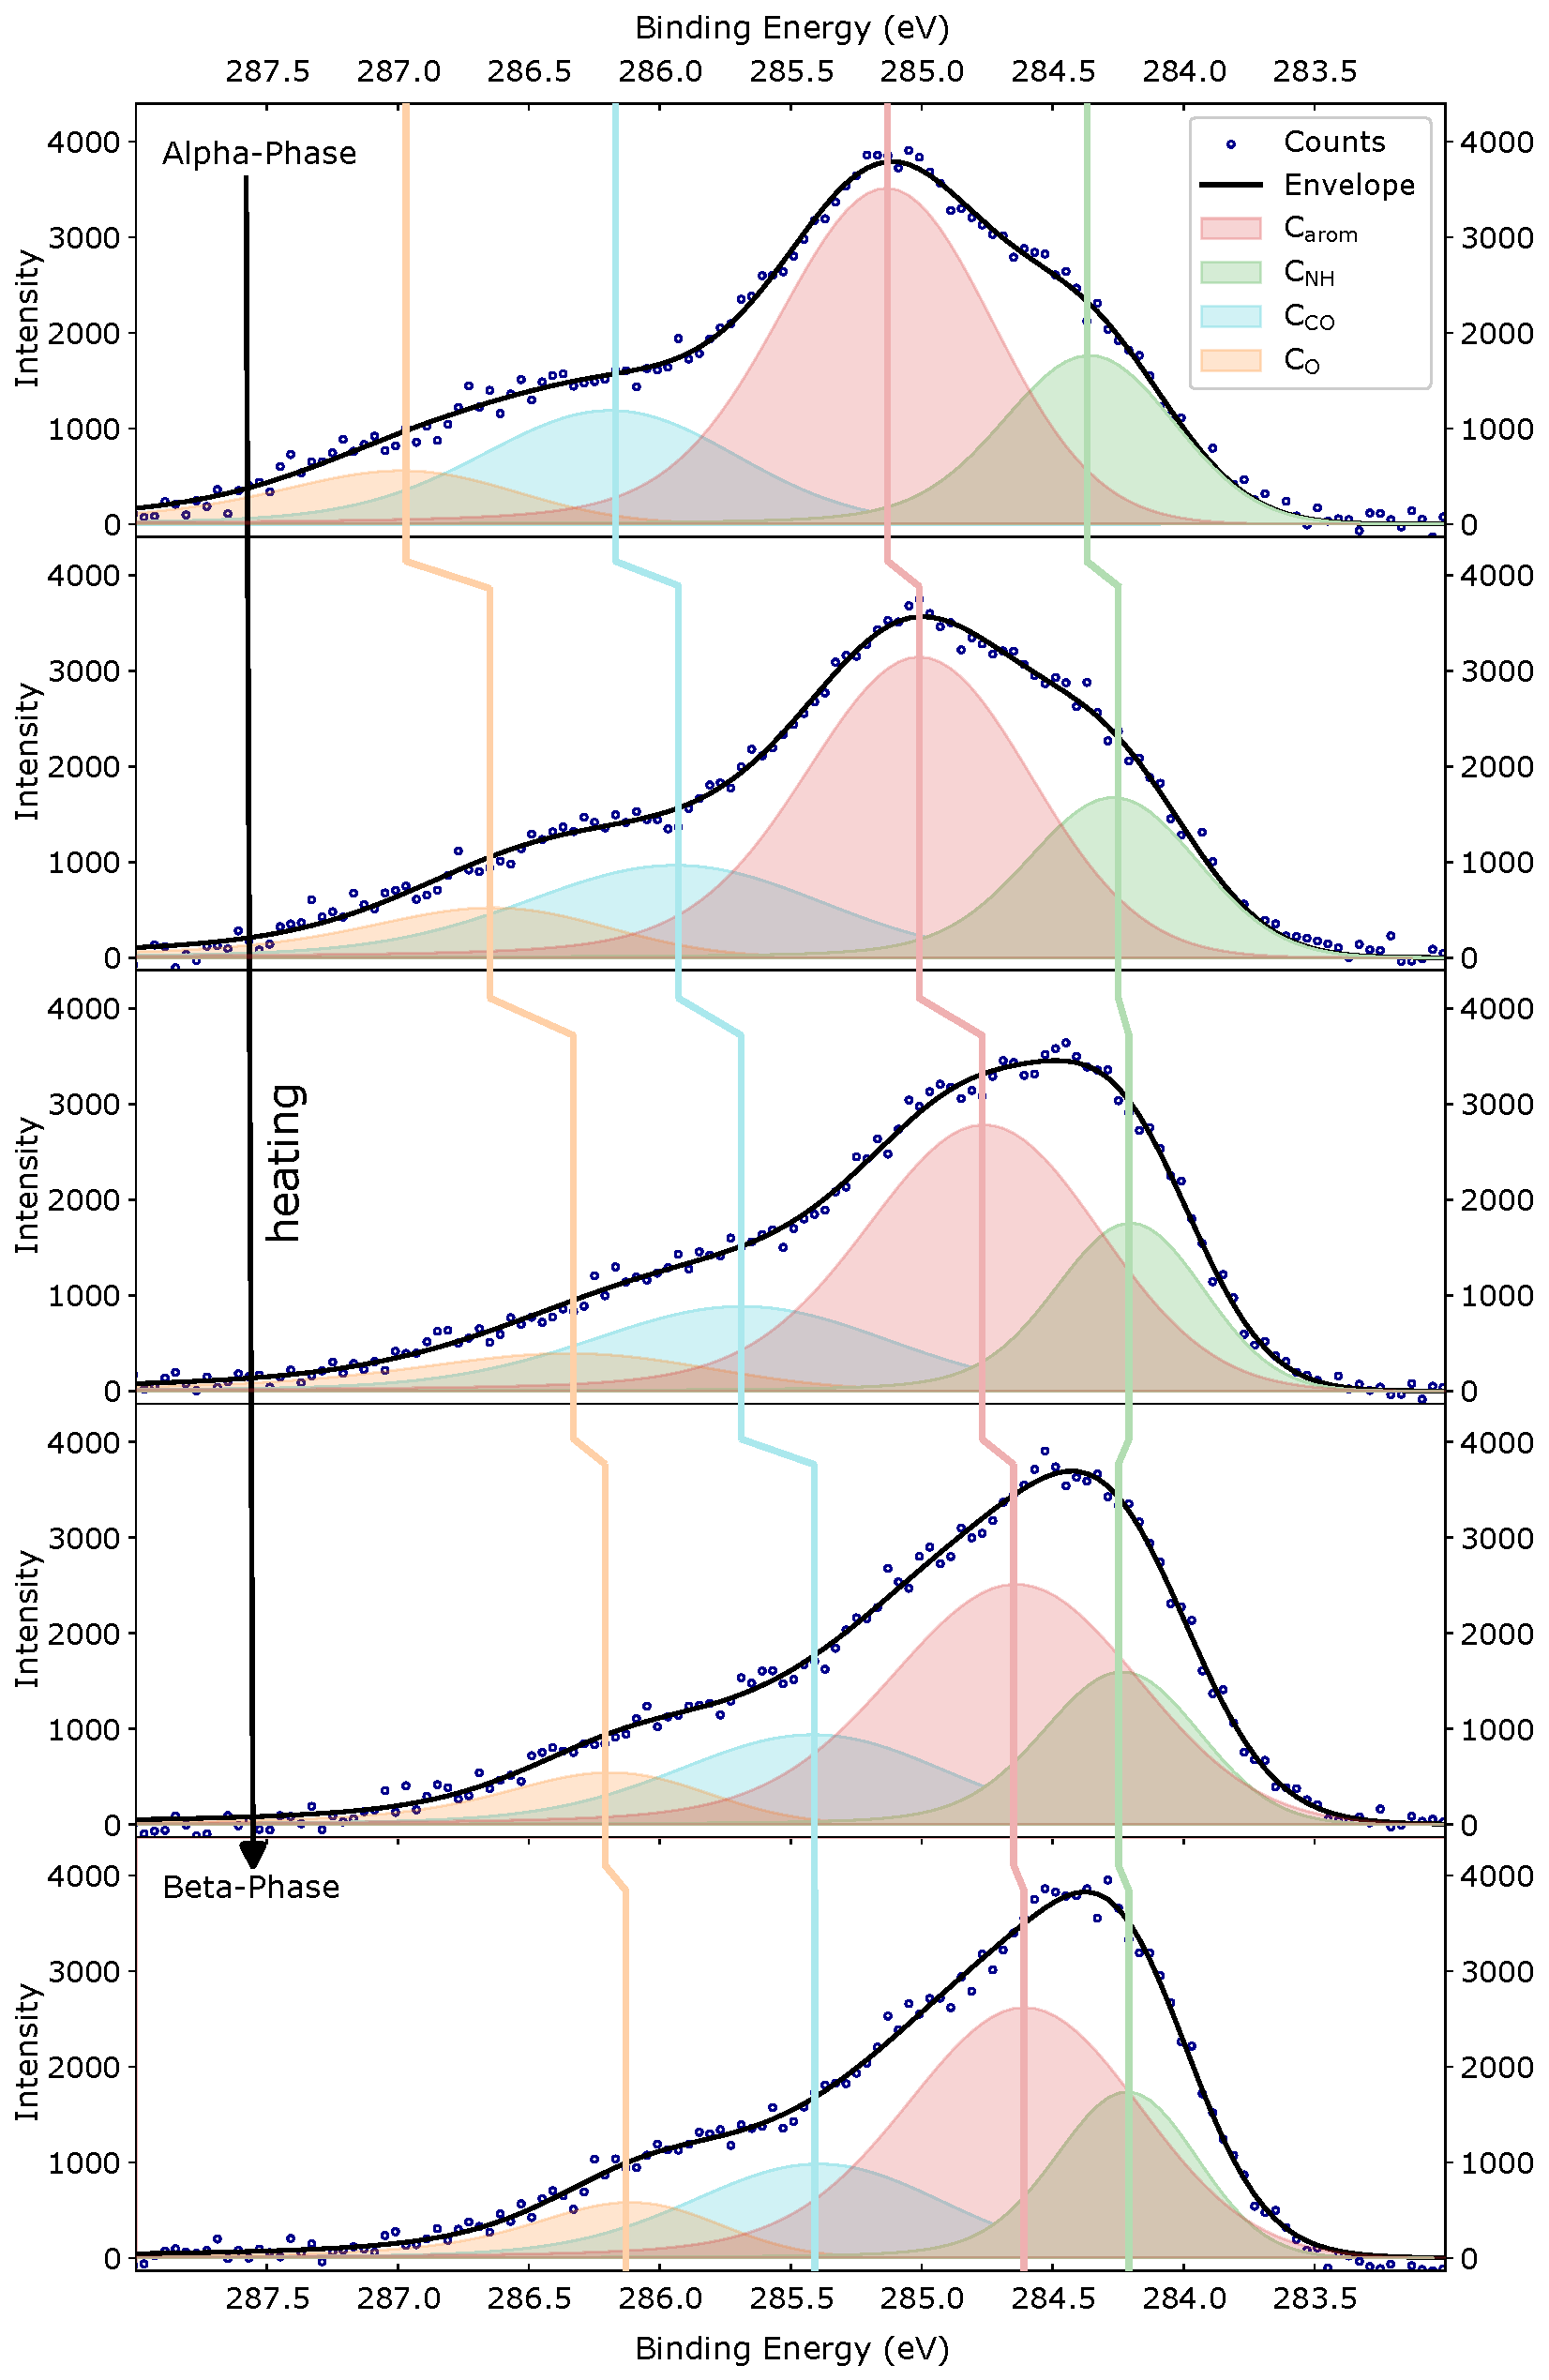
\includegraphics[width=0.93\textwidth]{images/C1s-phase-transition.pdf}
	\caption{C1s \ac{XPS} spectrum for the phase transition from the $\alpha$- to the $\beta$-phase of \ac{QA} on Ag(100).}
	\label{fig:C1s-phase-transition}
\end{figure}

\cleardoublepage
\section{The commensurate, 2D \texorpdfstring{$\beta$}{beta}-Phase}
\label{sec:res-beta}

The ensuing discourse will examine the phase designated as the $\beta$-phase. The investigation of the $\beta$-phase was conducted once more on all three available photoemission lines: C1s, O1s, and N1s. To address this need, the present chapter has been meticulously subdivided into discrete sections, each dedicated to specific photoemission lines. A comprehensive analysis of a particular \ac{XPS} spectrum of the $\beta$-phase is presented in each section, along with a comparative analysis of the $\alpha$- and $\beta$-phases.

\subsection{C1s spectra}

The C1s \ac{XPS} spectrum for the $\beta$-phase of \ac{QA} on Ag(100) is presented in \autoref{fig:C1s-beta}.

\begin{figure}[H]
	\centering
	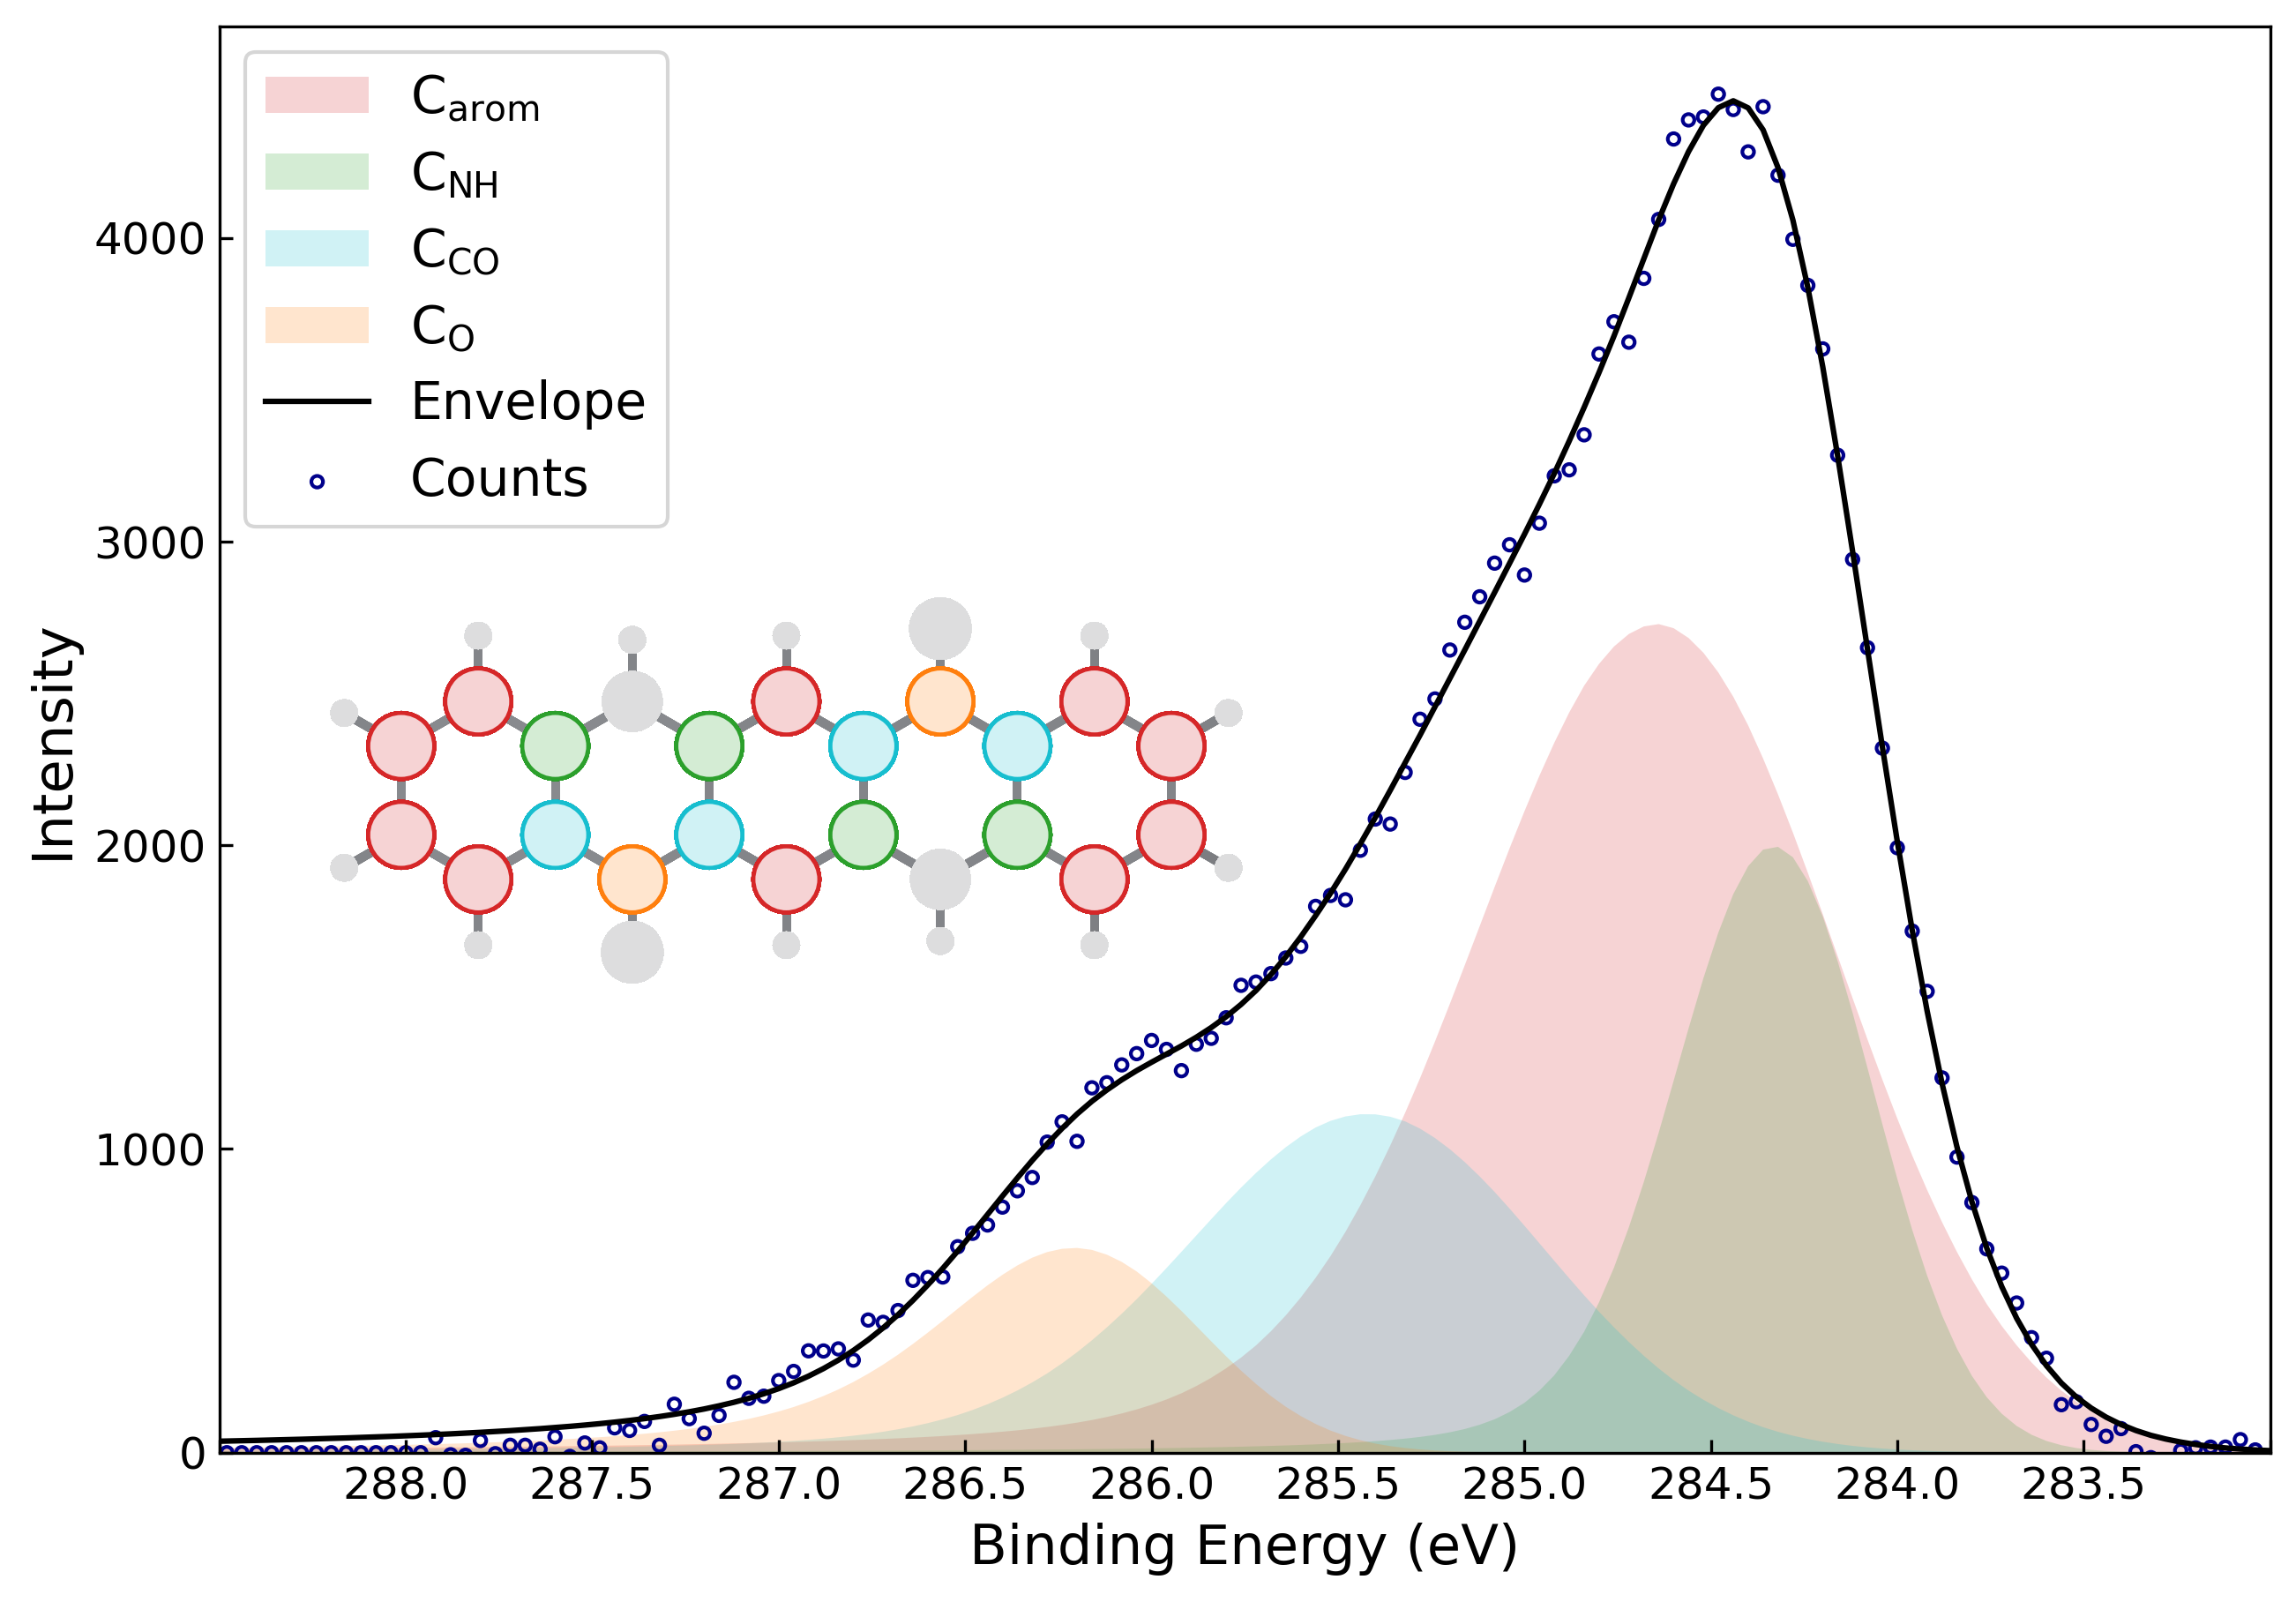
\includegraphics[width=0.9\textwidth]{images/C1s-beta.png}
	\caption{C1s \ac{XPS} spectrum for the $\beta$-phase of \ac{QA} on Ag(100).}
	\label{fig:C1s-beta}
\end{figure}

The \ac{XPS} spectrum of \ac{QA} in the $\beta$-phase displays four distinct components, designated as $\mathrm{C_{arom}}$, $\mathrm{C_{NH}}$, $\mathrm{C_{CO}}$ and $\mathrm{C_{O}}$, which bear the same nomenclature as in the $\alpha$-phase. This finding suggests that the various carbon atoms present within the \ac{QA} molecule exhibit a persistent correlation with distinct peaks in the \ac{XPS} spectrum.

The primary component, $\mathrm{C_{arom}}$, is located at a \ac{BE} of 284.545~\si{\eV} with a \ac{FWHM} of 1.132~\si{\eV}. The second peak, characterized by a \ac{BE} of 284.275~\si{\eV} and a \ac{FWHM} of 0.618~\si{\eV}, is identified as the $\mathrm{C_{NH}}$ peak. The $\mathrm{C_{CO}}$ peak is located at a \ac{BE} of 285.322~\si{\eV}, experiencing a \ac{FWHM} of 1.107~\si{\eV}. In the vicinity of this peak, at a higher \ac{BE}, is the $\mathrm{C_{O}}$ peak at 286.072~\si{\eV} with a \ac{FWHM} of 0.785~\si{\eV}.

A qualitative investigation of the peak areas yielded analogous results to those of the $\alpha$-phase, wherein the area ratios exhibited precise congruence with the number of carbon atoms in the \ac{QA} molecule.

In summary, the \ac{XPS} spectrum for C1s components of the $\beta$-phase offers significant insights into the chemical changes that occur between the $\alpha$- and $\beta$-phase. The single peaks are compared to each other, thereby providing information about the local environment around the carbon atoms.

\begin{table}[H]
	\centering
	\caption{Fit model of the $\beta$-phase for C1s.}
	\begin{tabular}{|c|c|c|c|}
		\hline
		peak & \ac{BE} / eV & area ratio & FWHM / eV \\
		\hline
		$\mathrm{C_{arom}}$ & 284.545 & 10 & 1.132 \\ \hline
		$\mathrm{C_{NH}}$ & 284.275 & 4 & 0.618 \\ \hline
		$\mathrm{C_{CO}}$ & 285.322 & 4 & 1.107 \\ \hline
		$\mathrm{C_{O}}$ & 286.072 & 2 & 0.785 \\ \hline
	\end{tabular}
	\label{tab:C1s-beta-fit}
\end{table}

In order to facilitate a more robust comparison of the $\beta$-phase to the $\alpha$-phase, the C1s \ac{XPS} spectra of these two phases are presented in \autoref{fig:C1s-alpha-beta}.

\begin{figure}[H]
	\centering
	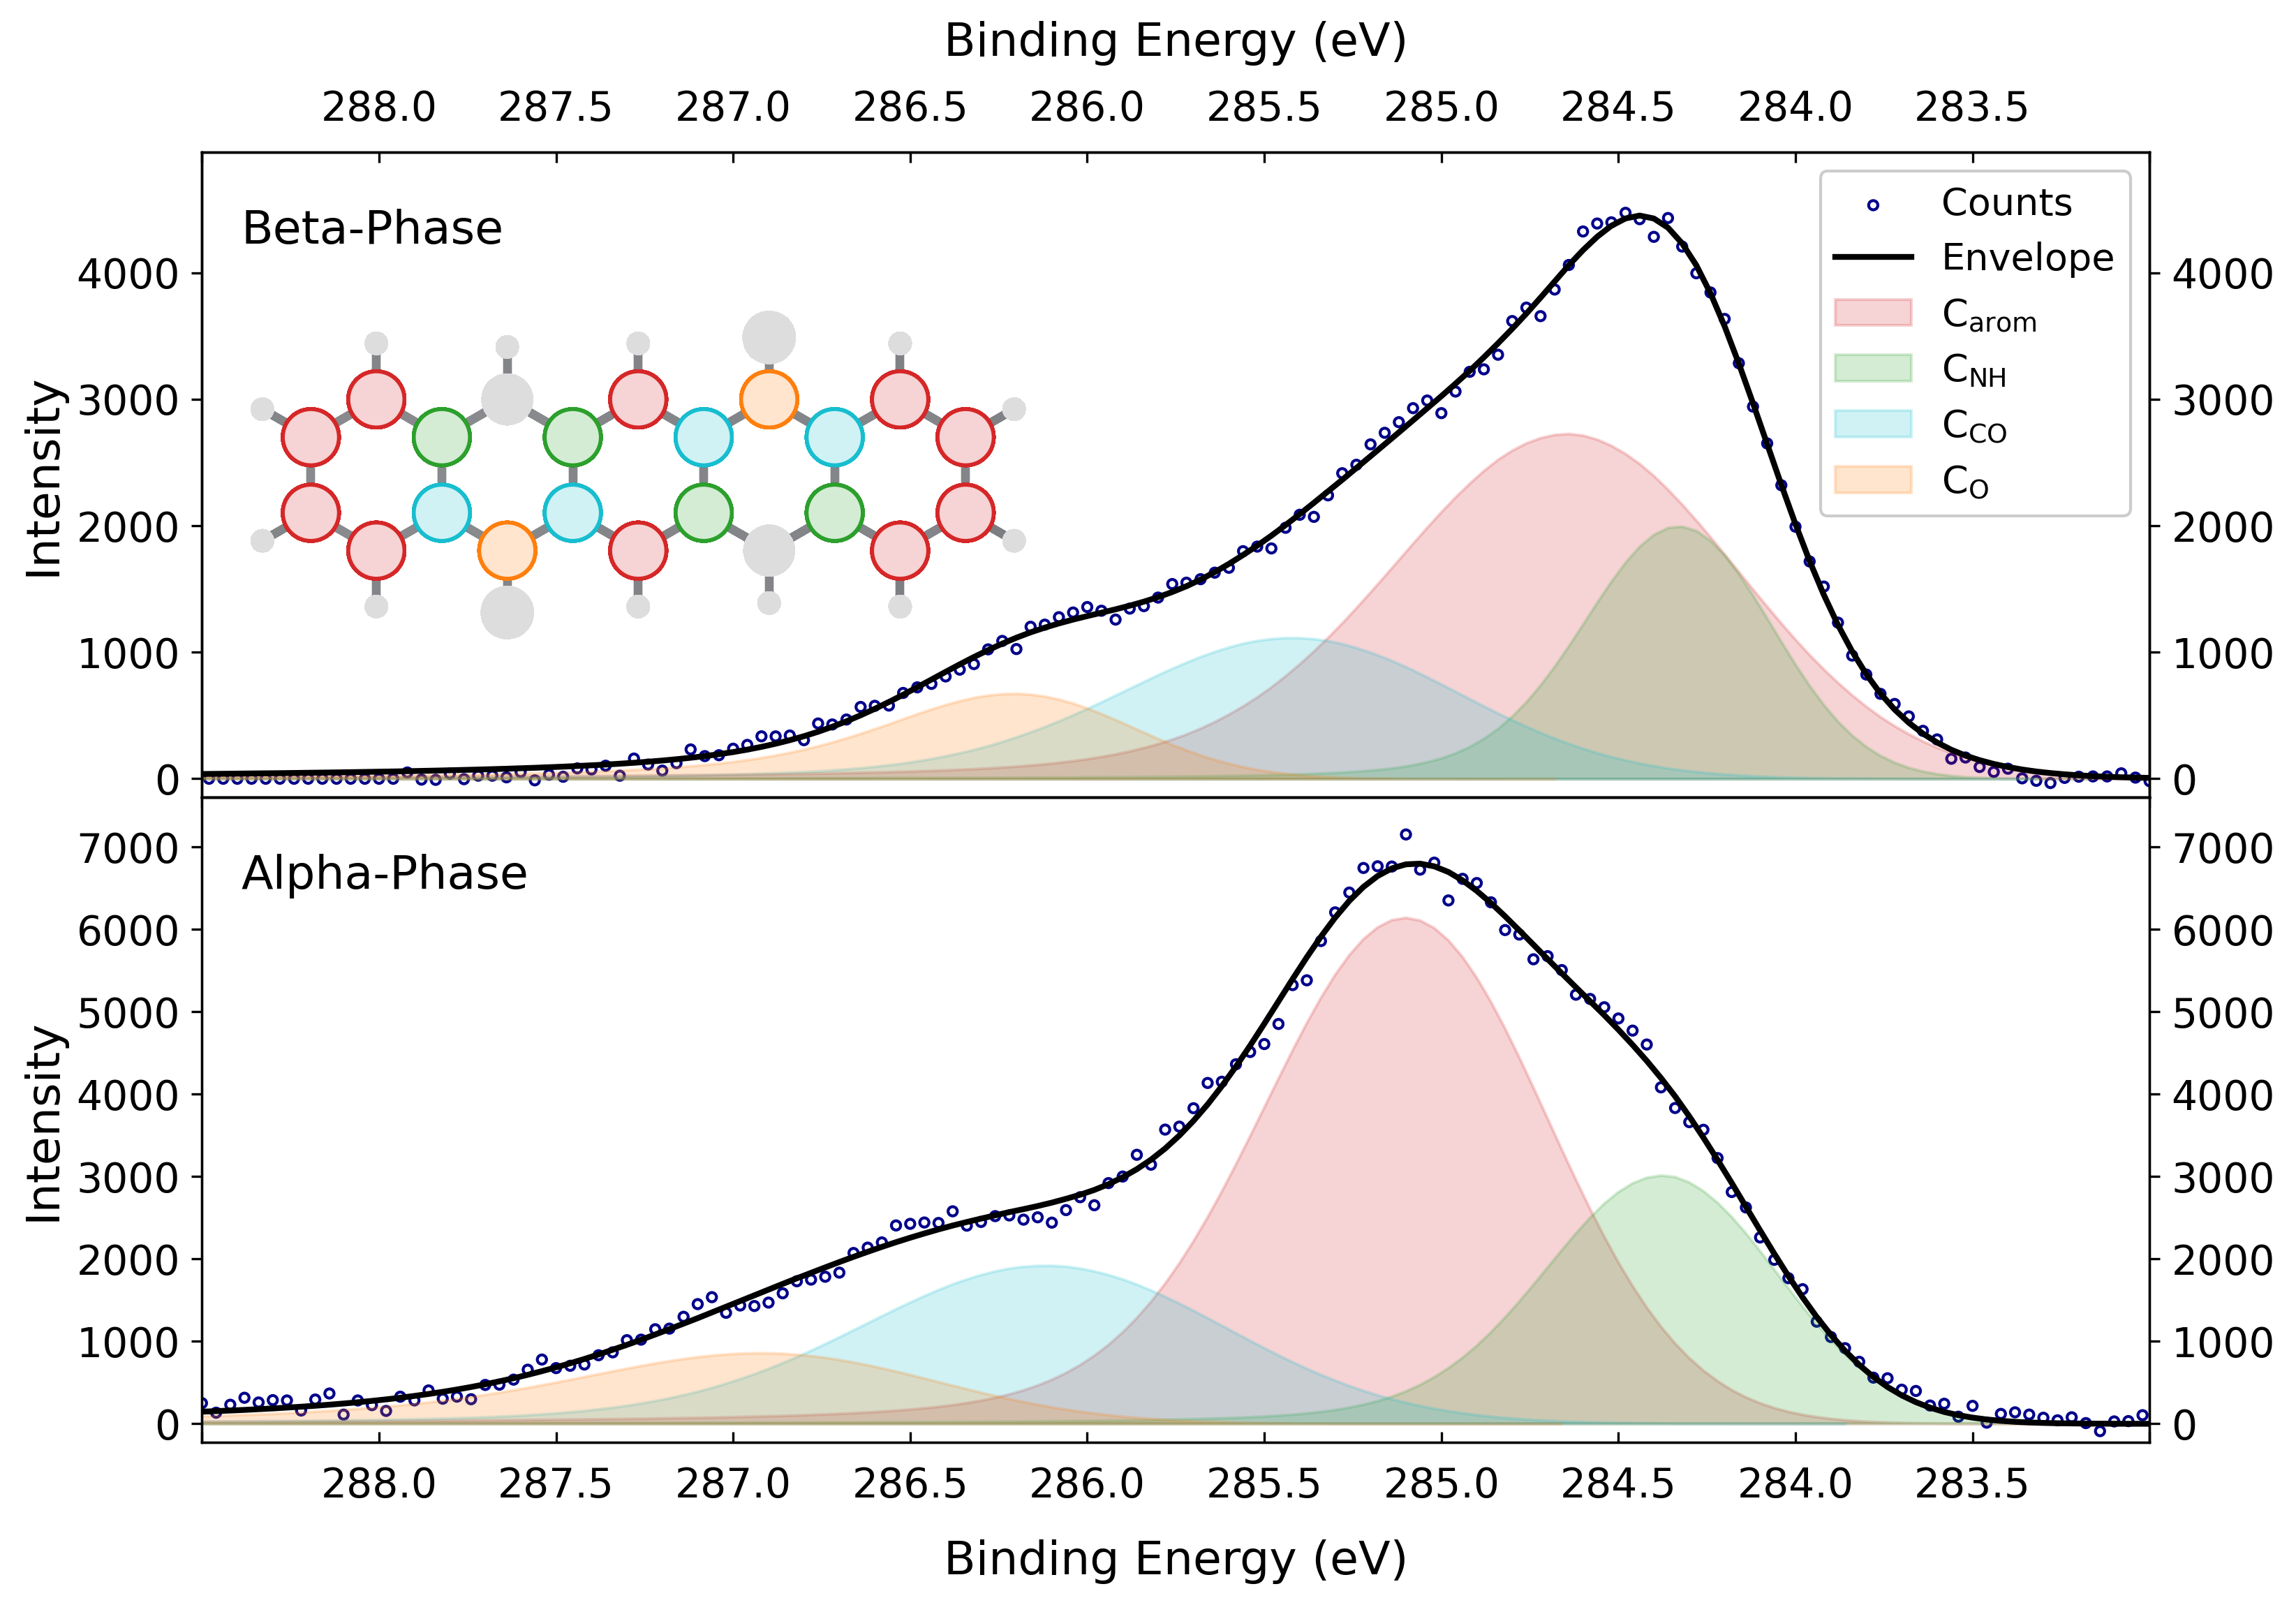
\includegraphics[width=0.9\textwidth]{images/C1s-phase-comparison.png}
	\caption{C1s \ac{XPS} spectrum for the $\alpha$- and $\beta$-phase  of \ac{QA} on Ag(100).}
	\label{fig:C1s-alpha-beta}
\end{figure}

A close examination reveals that all four peaks shift to a lower \ac{BE}. The shift in the \ac{BE} of the $\mathrm{C_{NH}}$ peak is, by far, the least significant. The three other peaks, $\mathrm{C_{arom}}$, $\mathrm{C_{CO}}$ and $\mathrm{C_{O}}$, demonstrate a comparable shift in the \ac{BE}.

A further noteworthy discrepancy is the increase of the \ac{FWHM} for the $\mathrm{C_{arom}}$ peak, which is approximately 0.19~\si{\eV}. The three other peaks demonstrate a decrease in their \ac{FWHM}. It is remarkable that the \ac{FWHM} of the $\mathrm{C_{O}}$ peak decreases by 0.37~\si{\eV}. The observed variation could be attributed to the underlying interconnectedness of all four peaks, which demonstrate a certain degree of interdependence.

In summary, the alterations in \acp{BE} and \ac{FWHM} values of the four peaks result in a significantly divergent \ac{XPS} spectrum. Consequently, \ac{QA} on Ag(100) in the $\beta$-phase is expected to demonstrate a comparable significant change compared to the $\alpha$-phase.

\cleardoublepage
\subsection{O1s spectra}

As illustrated in \autoref{fig:O1s-beta}, the \ac{XPS} spectrum for the O1s components for the $\beta$-phase of \ac{QA} on Ag(100) is presented.

\begin{figure}[H]
	\centering
	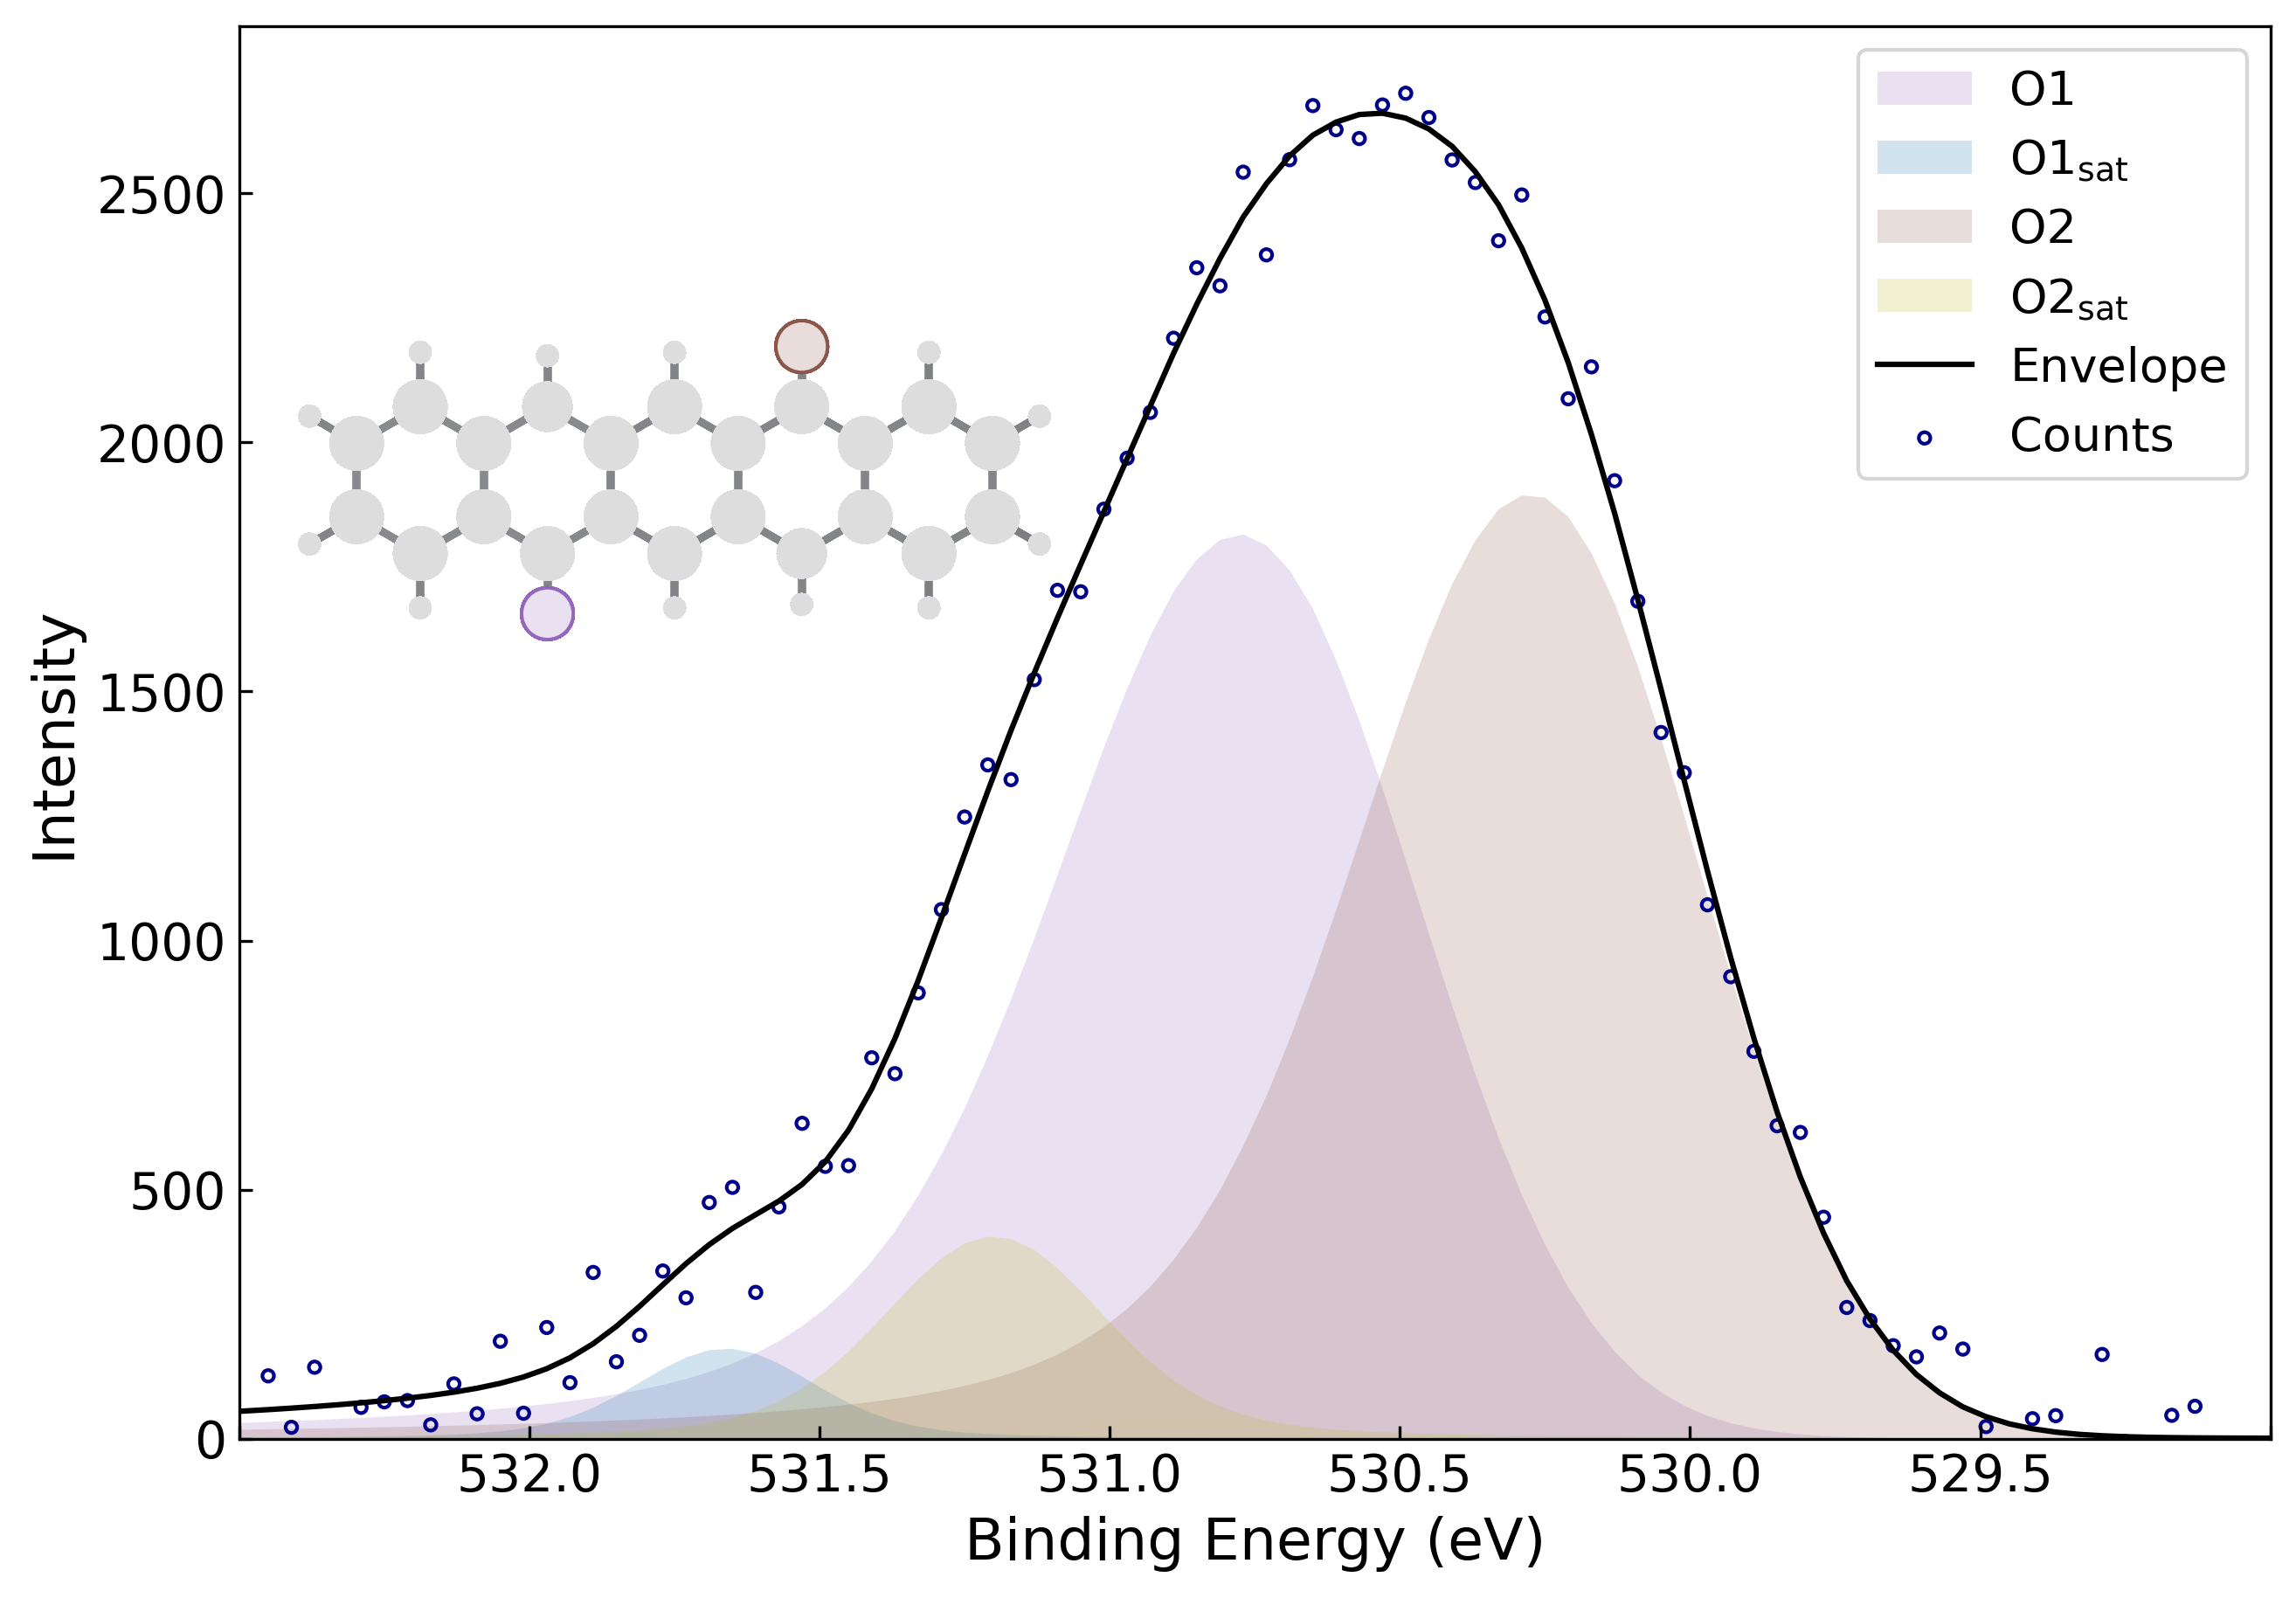
\includegraphics[width=0.9\textwidth]{images/O1s-beta.png}
	\caption{O1s \ac{XPS} spectrum for the $\beta$-phase of \ac{QA} on Ag(100).}
	\label{fig:O1s-beta}
\end{figure}

The \ac{XPS} spectrum of the $\beta$-phase in \autoref{fig:O1s-beta} consists of two peaks, each with its own satellite. The detailed data of the overall four peaks are shown in \autoref{tab:O1s-beta-fit}. The $\mathrm{O1}$ peak is located at a \ac{BE} of 530.683~\si{\eV} with a \ac{FWHM} of 0.712~\si{\eV}. The respective satellite is at 531.661~\si{\eV} with a \ac{FWHM} of 0.362~\si{\eV}. This corrresponds to a shift in \ac{BE} of 0.978~\si{\eV}.

The other peak, $\mathrm{O2}$, has a slightly lower \ac{BE} of 530.186~\si{\eV} but a similar \ac{FWHM} of 0.681~\si{\eV}. The satellite $\mathrm{O2_{sat}}$ also has a similar shift of 1.014~\si{\eV} and is located at a \ac{BE} of 531.200~\si{\eV} with a \ac{FWHM} of 0.451~\si{\eV}. The $\mathrm{O1}$ and $\mathrm{O2}$ have an area ratio of 1:1, which corresponds to one oxygen atom for each peak.

In summary, the \ac{FWHM} of two peaks are around 0.7~\si{\eV} and both have a shake-up satellite with a higher \ac{BE} by approximately 1.0~\si{\eV}. The two peaks are 0.5~\si{\eV} apart from each other.

\begin{table}[H]
	\centering
	\caption{Fit model of the $\beta$-phase for O1s.}
	\begin{tabular}{|c|c|c|c|}
		\hline
		peak & \ac{BE} / eV & area ratio & FWHM / eV \\
		\hline
		$\mathrm{O1}$ & 530.683 & 1 & 0.712 \\ \hline
		$\mathrm{O1_{sat}}$ & 531.661 & 0.05 & 0.362 \\ \hline
		$\mathrm{O2}$ & 530.186 & 1 & 0.681 \\ \hline
		$\mathrm{O2_{sat}}$ & 531.200 & 0.14 & 0.451 \\ \hline
	\end{tabular}
	\label{tab:O1s-beta-fit}
\end{table}

To enable a better comparison between $\alpha$- and $\beta$-phase, both spectra are depicted in \autoref{fig:O1s-alpha-beta}.

\begin{figure}[H]
	\centering
	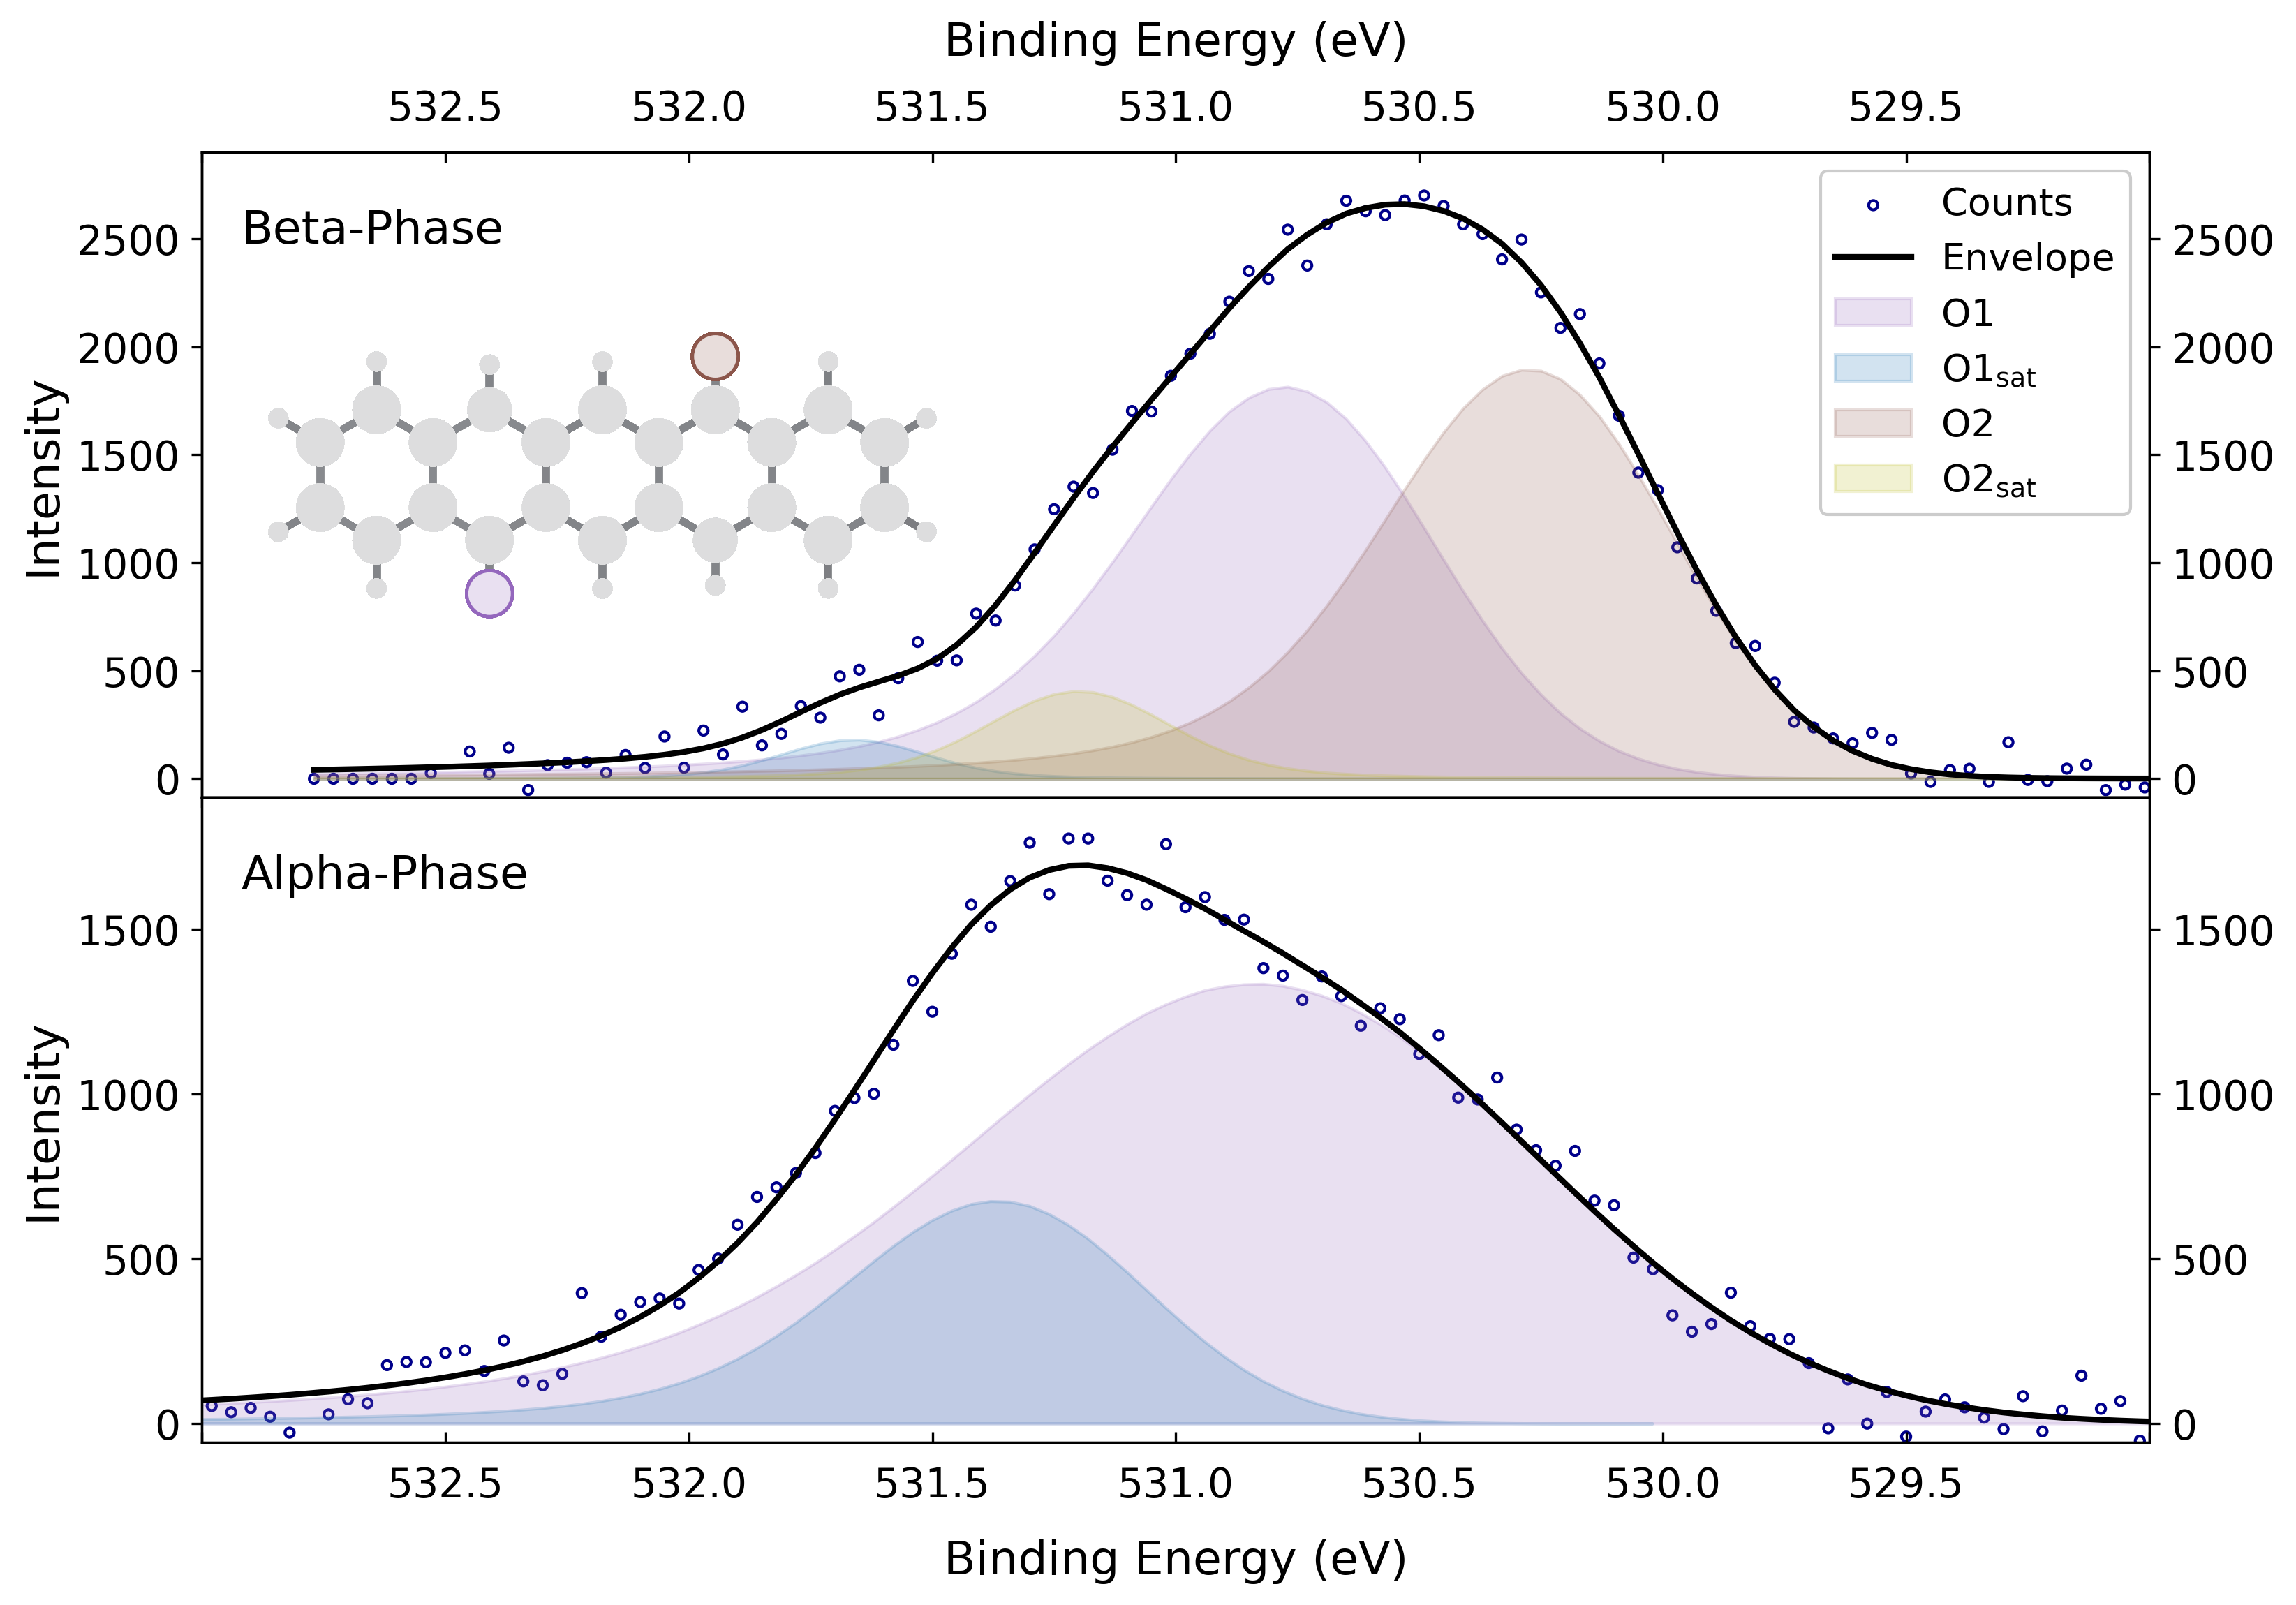
\includegraphics[width=0.9\textwidth]{images/O1s-phase-comparison.png}
	\caption{O1s \ac{XPS} spectrum for the $\alpha$- and $\beta$-phase  of \ac{QA} on Ag(100).}
	\label{fig:O1s-alpha-beta}
\end{figure}

The investigation of the differences between the two phases yields that the O1 peak does not change its position but exhibits a change in its \ac{FWHM} towards a smaller value. Same holds true for the $\mathrm{O1_{sat}}$ peak, which also changes its \ac{BE} by approximately 0.4~\si{\eV}.

The most significant change is obviously the second peak, occuring at the $\beta$-phase. This means that the two chemically equivalent peaks from the $\alpha$-phase have changed their environment, leading to two chemically different oxygen atoms in the $\beta$-phase.

\cleardoublepage
\subsection{N1s spectra}

As depicted in \autoref{fig:N1s-beta}, the N1s \ac{XPS} spectrum for the $\beta$-phase of \ac{QA} on Ag(100) has been presented.

\begin{figure}[H]
	\centering
	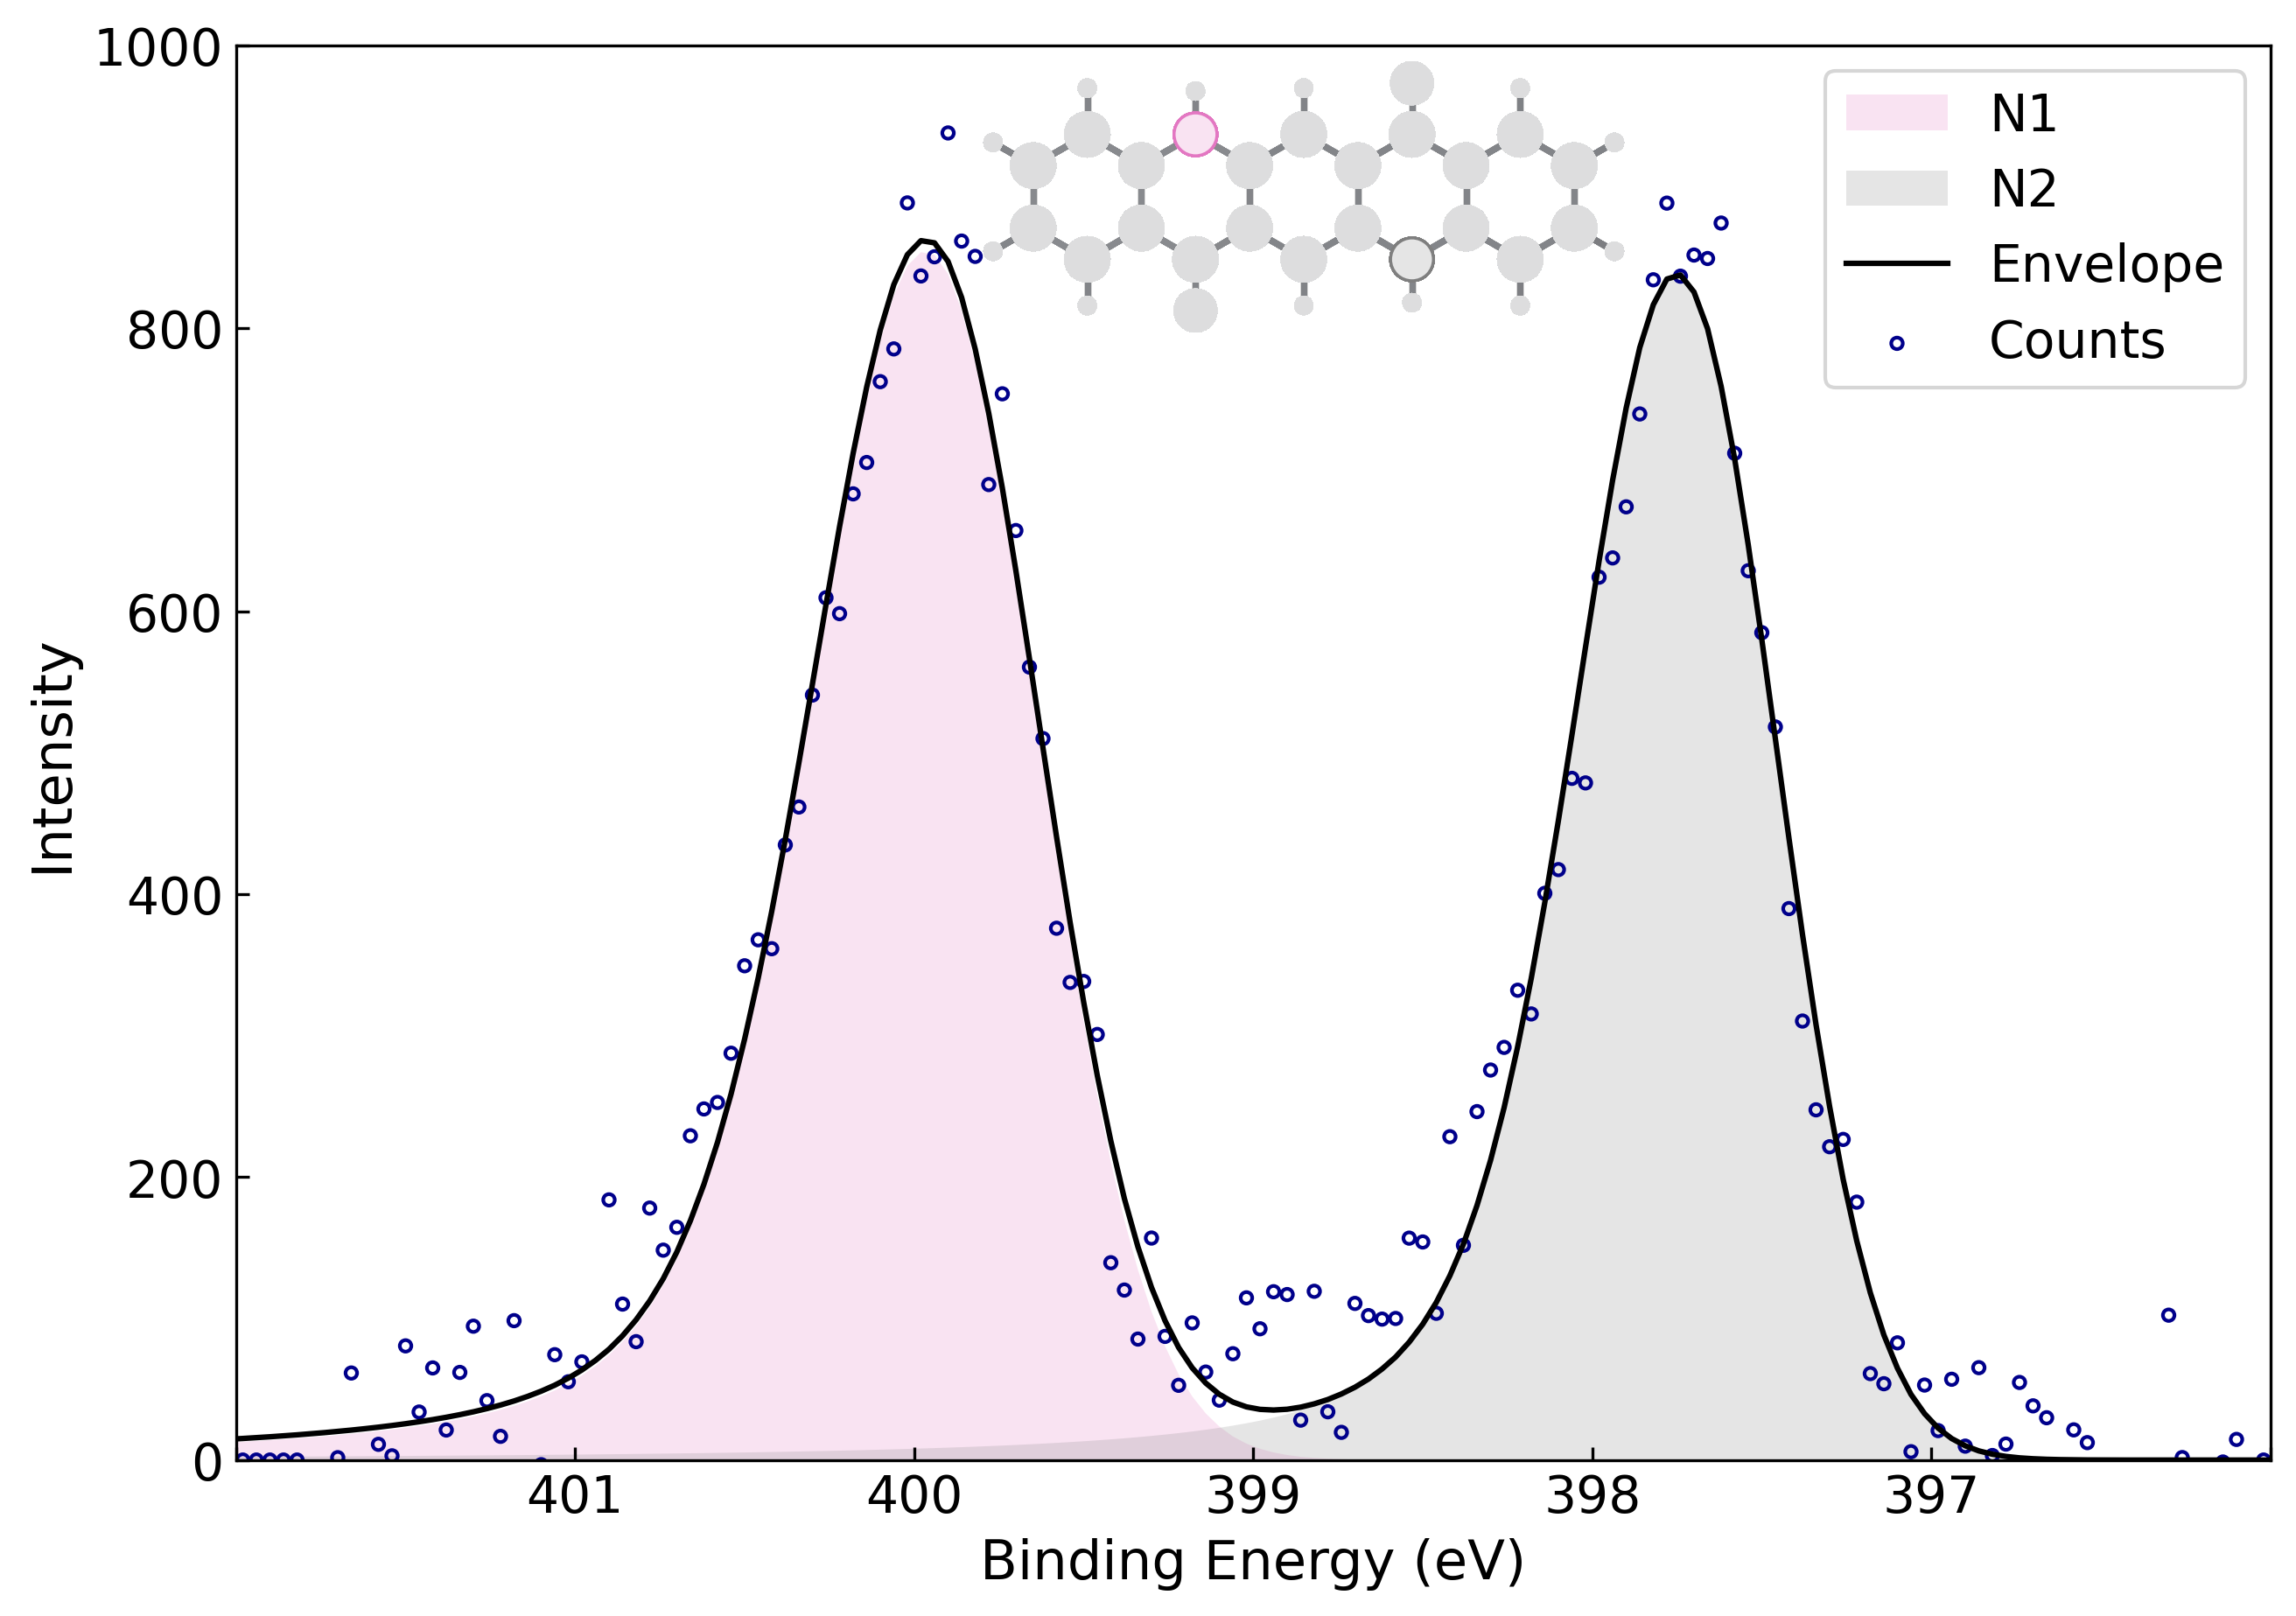
\includegraphics[width=0.9\textwidth]{images/N1s-beta.png}
	\caption{N1s \ac{XPS} spectrum for the $\beta$-phase of \ac{QA} on Ag(100).}
	\label{fig:N1s-beta}
\end{figure}

\autoref{fig:N1s-beta} and \autoref{tab:N1s-beta-fit} enable a quantitative description of the N1s \ac{XPS} spectrum for the $\beta$-phase. As seen, the $\beta$-phase has two different peaks for N1s, namely N1 and N2. Both peaks have a similar \ac{FWHM} of 0.774~\si{\eV} and 0.686~\si{\eV}. Furthermore, they have the same intensitiy and an area-ratio of 1:1. This indicates that each peak corresponds to one of the nitrogen atoms of \ac{QA}.

The main difference of the two peaks is their \ac{BE}. The N1 peak is located at a \ac{BE} of 399.865~\si{\eV} while the N2 peak has a \ac{BE} of 397.661~\si{\eV}. This means that the peaks are seperated by 2.20~\si{\eV}. In comparison to the shifts in \acp{BE} for the other photoemission lines, this value seems to indicate a quite drastic change in the chemical environment of one of the nitrogen atoms.

\begin{table}[H]
	\centering
	\caption{Fit model of the $\beta$-phase for N1s.}
	\begin{tabular}{|c|c|c|c|}
		\hline
		peak & \ac{BE} / eV & area ratio & FWHM / eV \\
		\hline
		$\mathrm{N1}$ & 399.865 & 1 & 0.774\\ \hline
		$\mathrm{N2}$ & 397.661 & 1 & 0.686 \\ \hline
	\end{tabular}
	\label{tab:N1s-beta-fit}
\end{table}

To enable a comparative analysis between the $\alpha$- and the $\beta$-phase, the two phases are depicted in a juxtaposed arrangement in \autoref{fig:N1s-alpha-beta}.

\begin{figure}[H]
	\centering
	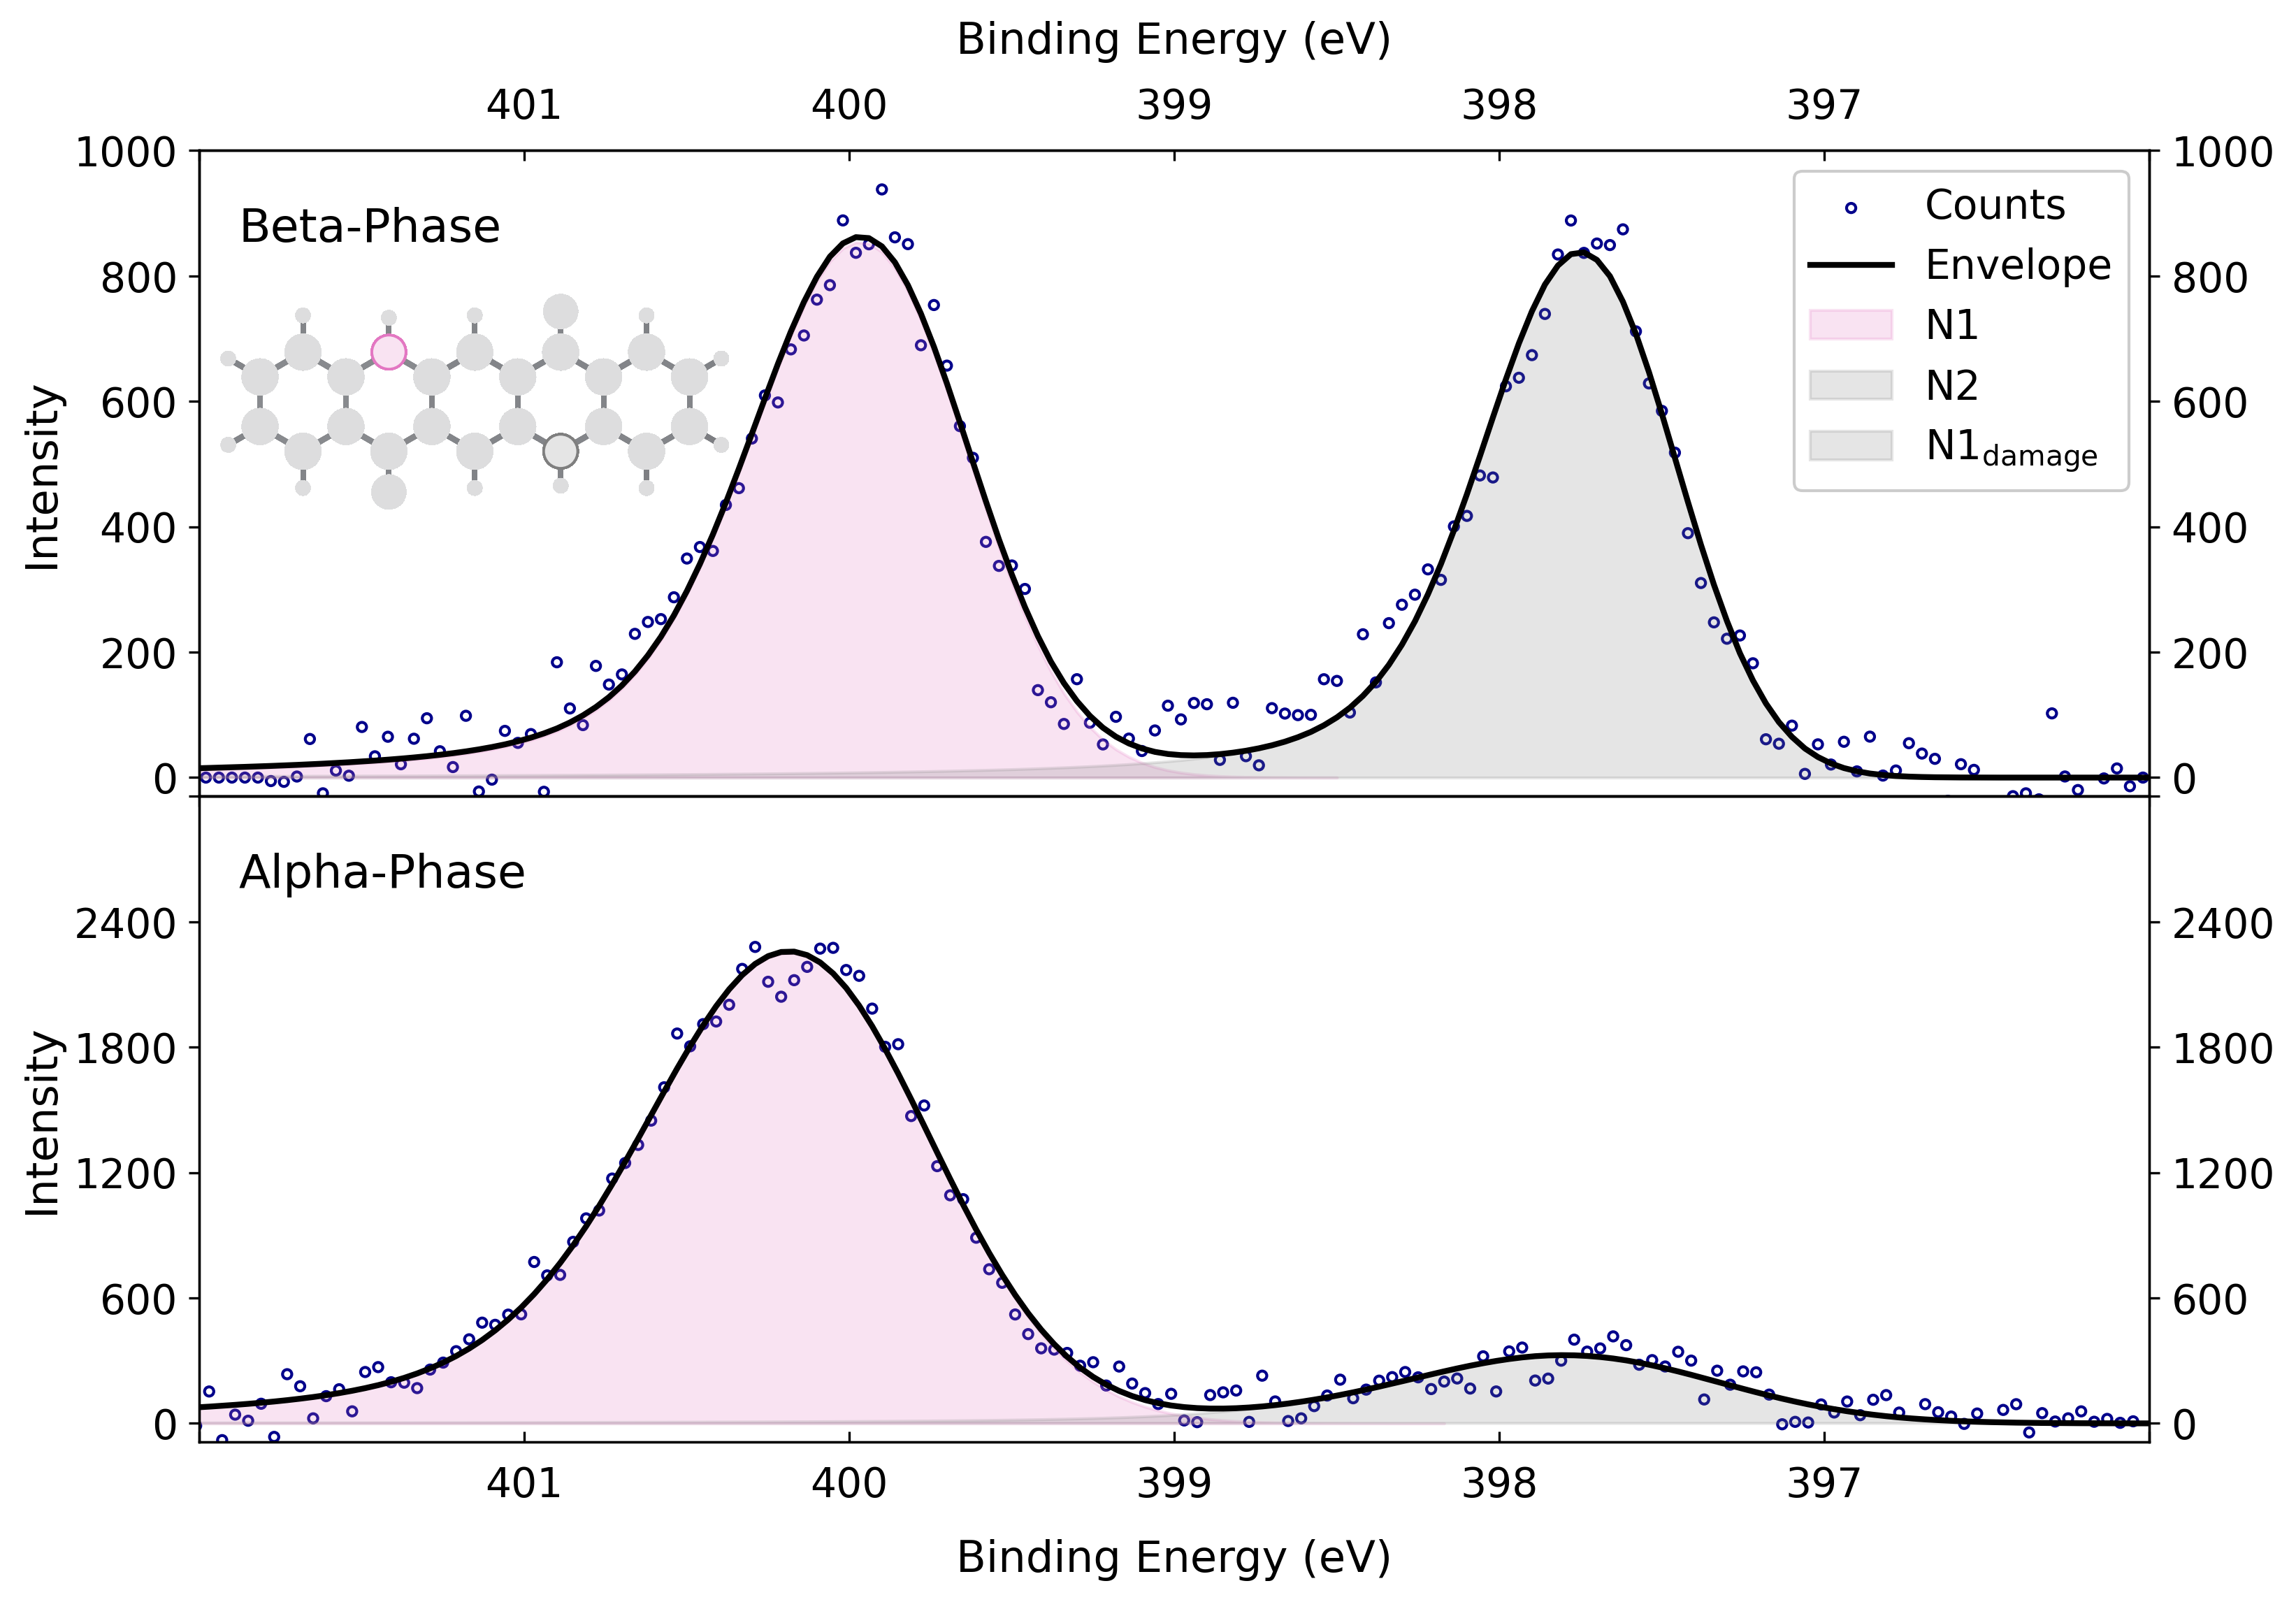
\includegraphics[width=0.9\textwidth]{images/N1s-phase-comparison.png}
	\caption{N1s \ac{XPS} spectrum for the $\alpha$- and $\beta$-phase of \ac{QA} on Ag(100).}
	\label{fig:N1s-alpha-beta}
\end{figure}

The comparison of the $\alpha$- and the $\beta$-phase yields interesting results about the nitrogen atoms. First, the N1 peak keeps almost the same \ac{BE} in both phases. There is only a change in \ac{BE} of about 0.188~\si{\eV} towards a lower value. The more significant change can be observed in the change of the \ac{FWHM}, decreasing from 1.017~\si{\eV} to 0.774~\si{\eV}. This corresponds to a sharper peak in the \ac{XPS} spectrum, indicating a more homogenous environment for the N1 peak.

Nevertheless, the other peak, namely N2, reveals a more intriguing finding, prompting further examination. The N2 peak has exactly the same \ac{BE} as the $\mathrm{N1_{damage}}$ peak of the $\alpha$-phase. As seen in \autoref{fig:N1s-alpha-beta}, the areas of the N2 peak in the different phases can not be compared anyhow, which also makes an comparison of the \ac{FWHM} unsuitable.


\cleardoublepage
\section{Binding energy changes upon phase transition}

For a further comparison of the differences in the \acp{BE} between the $\alpha$- and the $\beta$-phase, an overview of these are illustrated in \autoref{fig:phase-shift}.

\begin{figure}[H]
	\centering
	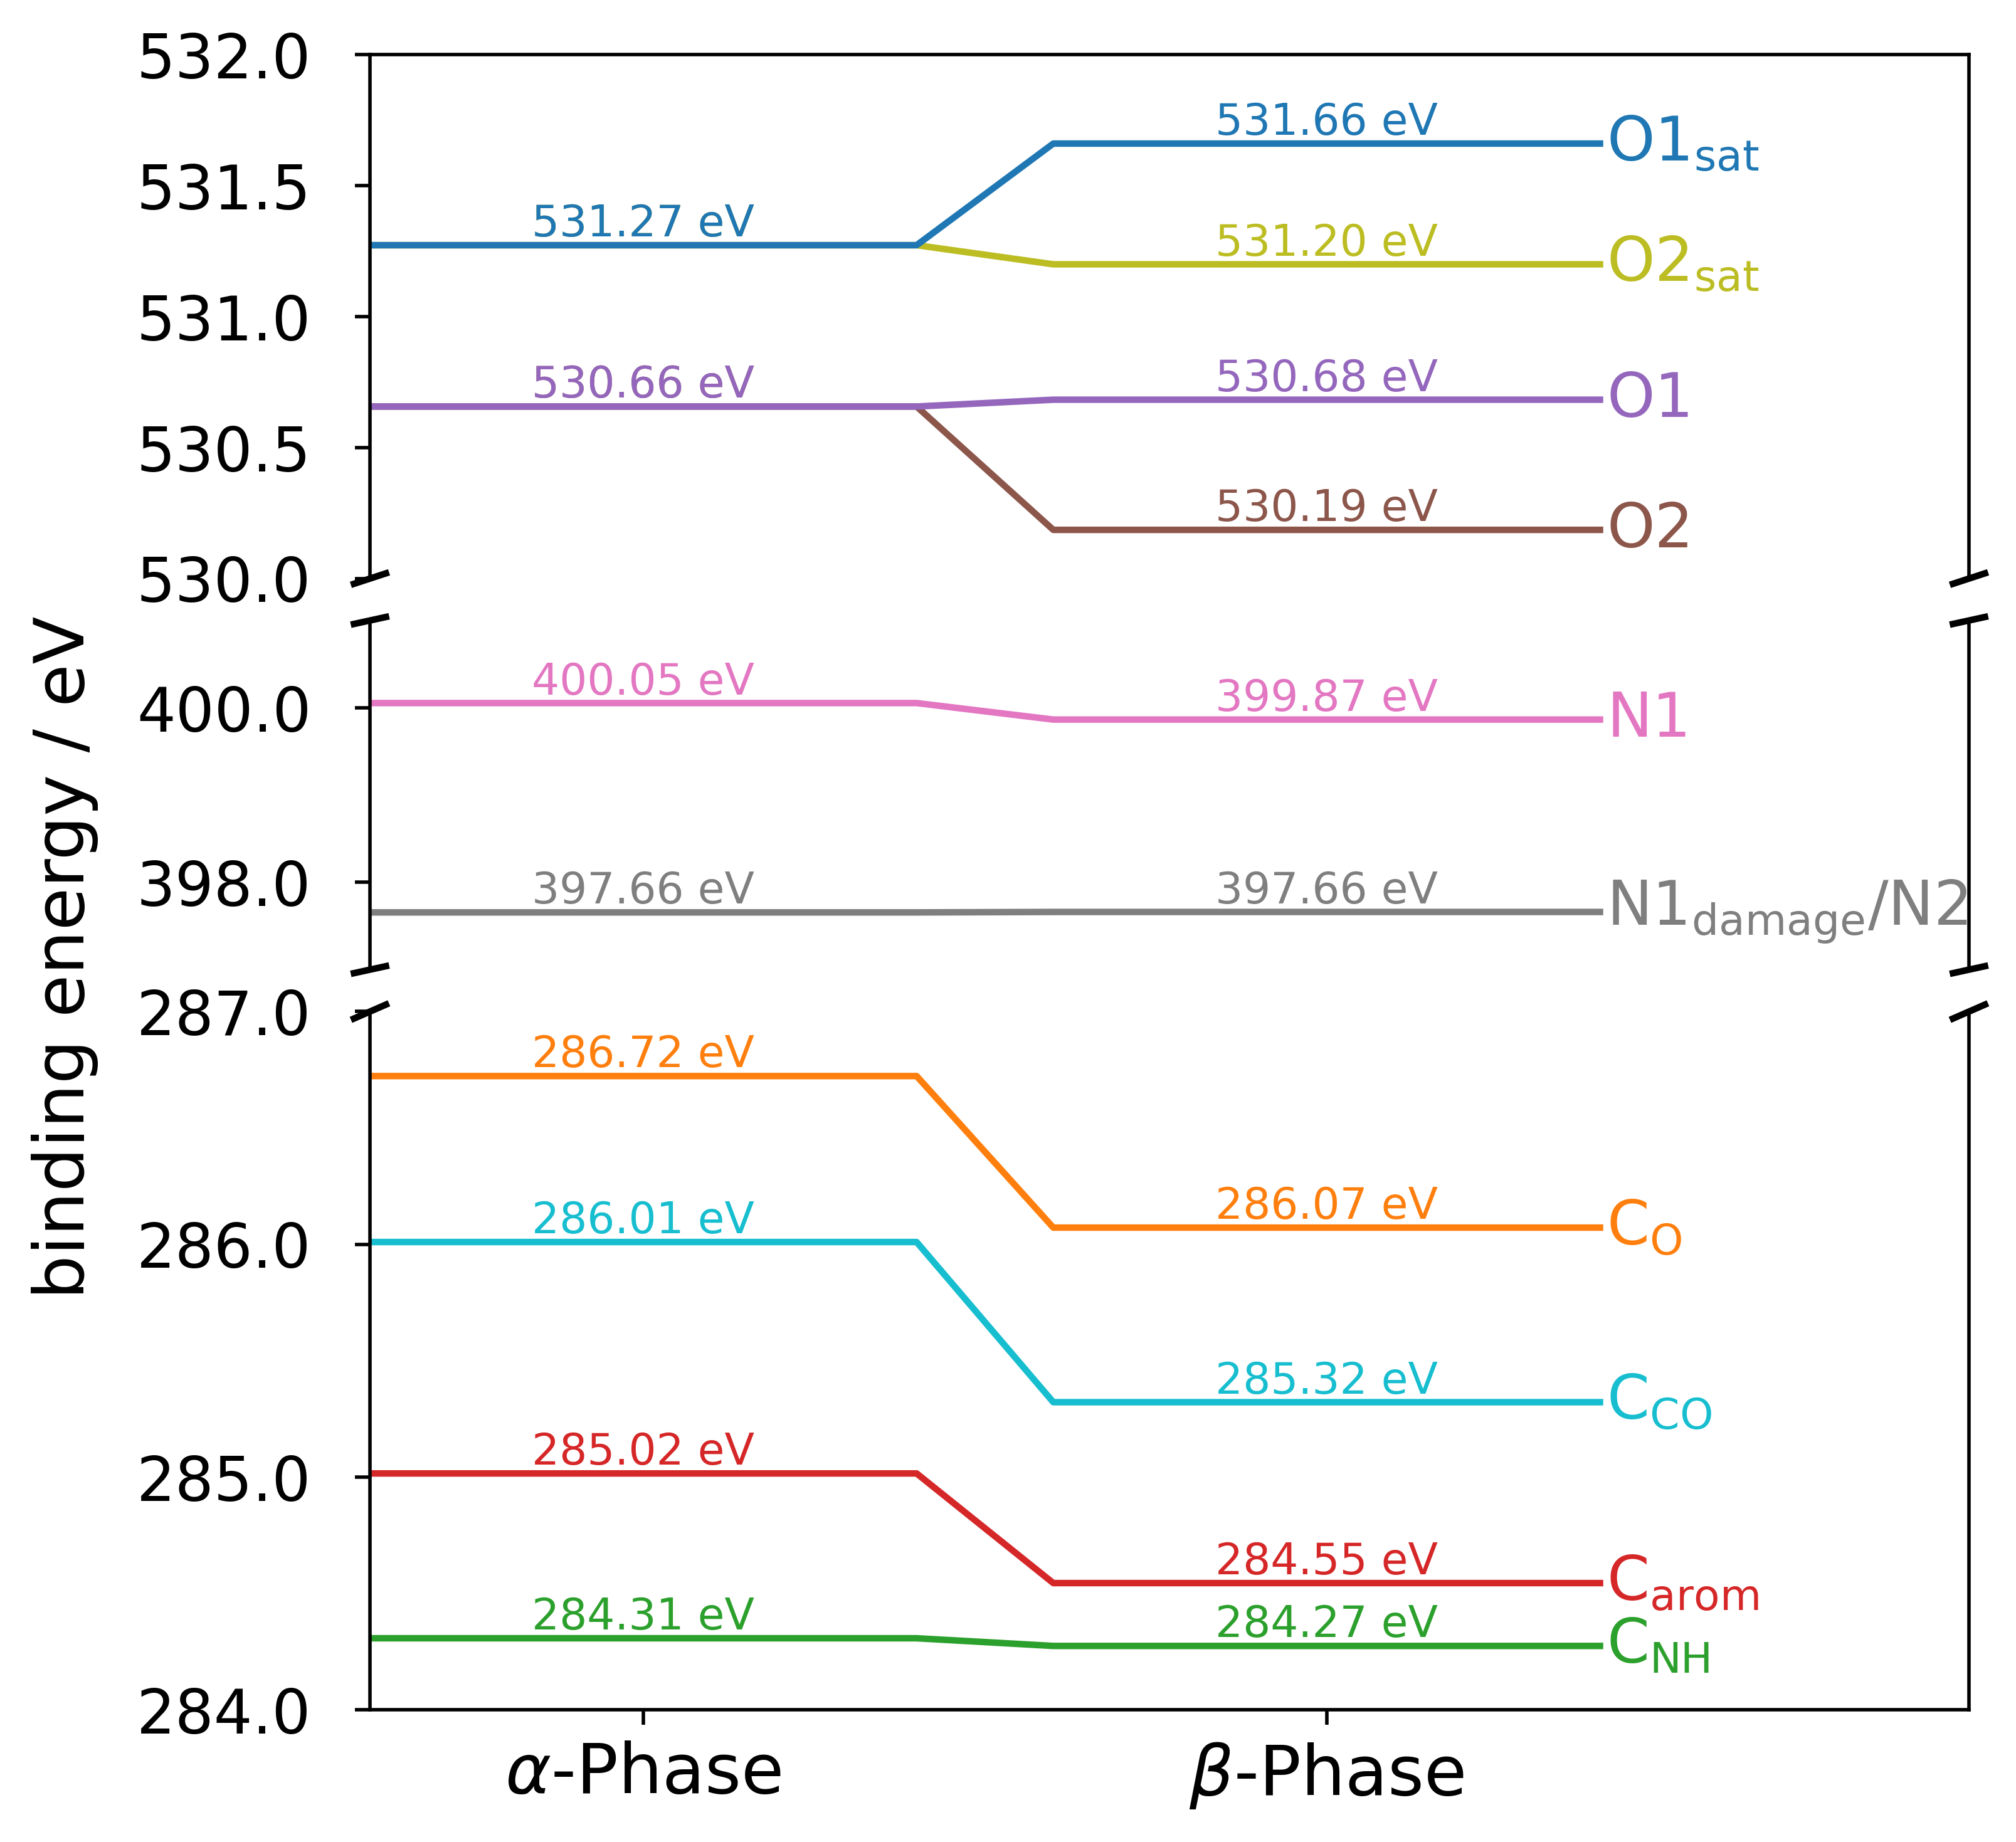
\includegraphics[width=0.95\textwidth]{images/phase-shifts.png}
	\caption{Illustration of the shift in the \ac{BE} from the $\alpha$- to the $\beta$-phase of \ac{QA} on Ag(100) for the different peaks in the \ac{XPS} spectra for all core-levels.}
	\label{fig:phase-shift}
\end{figure}

Initially, a significant trend is observed in all peaks across all \ac{XPS} spectra. The \acp{BE} of all atoms in the $\beta$-phase are a lower than or similar to those of the atoms in the $\alpha$-phase.

Starting with the \ac{XPS} spectra for C1s, the differences in the \acp{BE} are subsequently examined in detail. Shifts in the \ac{BE} for three of the four peaks, namely $\mathrm{C_{arom}}$, $\mathrm{C_{CO}}$ and $\mathrm{C_{O}}$ are similar. They all decrease by 0.5-0.7~\si{\eV}. Conversely, the \ac{BE} of the $\mathrm{C_{NH}}$ peak does not significantly decrease. This indicates that the carbon atoms next to the amine undergo a different change during phase transition than the other carbon atoms.

Consequently, the \ac{XPS} spectra for N1s are of great interest. As previously mentioned, the $\beta$-phase exhibits two peaks instead of one for N1s. The second peak in the $\beta$-phase is more than 2 ~\si{\eV} lower in \ac{BE} than the first peak. This represents a significant difference in the \ac{BE} that is not observed for any other peak. To provide an example, the \ac{BE} difference between the $\mathrm{C_{NH}}$ and the $\mathrm{C_{O}}$ peak, despite their very different chemical environments, is only 1.8~\si{\eV}.

Lastly, the \acp{BE} of the two phases for the O1s \ac{XPS} spectra are compared. Again, there are two distinct peaks in the $\beta$-phase instead of one in the $\alpha$-phase. The \ac{BE} of one peak remains at roughly the same value, while the other decreases by about 0.4~\si{\eV}. This result is similar to the change in \ac{BE} observed in the C1s \ac{XPS} spectra.

\cleardoublepage
